%%%%%%%%%%%%%%%%%%%%%%%%%%%%%%%%%%%%%%%%%%%%%%%%%%%%%%%%%%%%%%%%%%%%%%%%%%
%% Trim Size: 9.75in x 6.5in
%% Text Area: 8in (include Runningheads) x 5in
%% ws-ijhr.tex   :  9-5-2005 
%% Tex file to use with ws-ijhr.cls written in Latex2E.
%% The content, structure, format and layout of this style file is the
%% property of World Scientific Publishing Co. Pte. Ltd.
%% Copyright 1995, 2003 by World Scientific Publishing Co.
%% All rights are reserved.
%%%%%%%%%%%%%%%%%%%%%%%%%%%%%%%%%%%%%%%%%%%%%%%%%%%%%%%%%%%%%%%%%%%%%%%%%%%%
%

%%%%%%%%%%%%% FOR TEMPLATE OF TYPING OUT THE BIBLIOGRAPHY TEXT ONLY %%%%%%%%
\newcounter{myctr}
\def\myitem{\refstepcounter{myctr}\bibfont\parindent0pt\hangindent13pt\themyctr.\enskip}
\def\myhead#1{\vskip10pt\noindent{\bibfont #1:}\vskip4pt}
%%%%%%%%%%%%% FOR TEMPLATE OF TYPING OUT THE BIBLIOGRAPHY TEXT ONLY %%%%%%%%

\documentclass{ws-ijhr}

\hyphenation{op-tical net-works semi-conduc-tor}

\usepackage{graphicx}
\usepackage{multicol}
\usepackage{multirow}
\usepackage[bookmarks=true]{hyperref}
\usepackage{amssymb,amsmath}
\usepackage{subfig}
\usepackage{bbding}

\newcommand{\eq}{Eq.~}
\newcommand{\fig}{Fig.~}
\newcommand{\tab}{Tab.~}
\newcommand{\sect}{Sec.~}

\newcommand{\re}{R}
\newcommand{\rf}{R}
\newcommand{\rl}{L}
\newcommand{\om}{O}
\newcommand{\cm}{M}
\newcommand{\fm}{F}
\newcommand{\hc}{C}
\newcommand{\qd}{Q}
\newcommand{\gpm}{T}
\newcommand{\coll}{W}
\newcommand{\pdf}{\mathbf{pdf}}

\newcommand{\argmax}[1]{\underset{#1}{\operatorname{argmax}}\medspace}

\begin{document}

\markboth{Umit Rusen Aktas, Chao Zhao, Marek Kopicki, Ales Leonardis, Jeremy L. Wyatt}{Deep Dexterous Grasping of Novel Objects from a Single View}

%%%%%%%%%%%%%%%%%%%%% Publisher's Area please ignore %%%%%%%%%%%%%%%
%
\catchline{}{}{}{}{}
%
%%%%%%%%%%%%%%%%%%%%%%%%%%%%%%%%%%%%%%%%%%%%%%%%%%%%%%%%%%%%%%%%%%%%

\title{Deep Dexterous Grasping of Novel Objects from a Single View}

\author{UMIT RUSEN AKTAS}

\address{University Department, University Name, Address\\
City, State ZIP/Zone,
Country\\
rusenaktas@gmail.com}

\author{CHAO ZHAO}

\address{Group, Laboratory, Address\\
City, State ZIP/Zone, Country\\
chaozh1@hotmail.com}

\author{MAREK KOPICKI}

\address{Group, Laboratory, Address\\
City, State ZIP/Zone, Country\\
marekkopicki@gmail.com}

\author{ALES LEONARDIS}

\address{Group, Laboratory, Address\\
City, State ZIP/Zone, Country\\
alesleo@gmail.com}

\author{JEREMY L. WYATT}

\address{Group, Laboratory, Address\\
City, State ZIP/Zone, Country\\
jeremy.l.wyatt@gmail.com}

\maketitle

\begin{history}
\received{1 Jan 2021} %
\revised{1 Jan 2021}  %
\accepted{1 Jan 2021} %
%\comby{(xxxxxxxxxx)}
\end{history}

\begin{abstract}
Dexterous grasping of a novel object given a single view is an open problem. This paper makes several contributions to its solution. First, we present a simulator for generating and testing dexterous grasps. Second we present a data set, generated by  this simulator, of 2.4 million simulated dexterous grasps of variations of 294 base objects drawn from 20 categories. Third, we present a basic architecture for generation and evaluation of dexterous grasps that may be trained in a supervised manner. Fourth, we present three different evaluative architectures, employing ResNet-50 or VGG16 as their visual backbone. Fifth, we train, and evaluate seventeen variants of generative-evaluative architectures on this simulated data set, showing improvement from 69.53\% grasp success rate to 90.49\%. Sixth, we present a real robot implementation and evaluate the four most promising variants, executing 196 real robot grasps in total. We show that our best architectural variant achieves a grasp success rate of 87.8\% on real novel objects seen from a single view, improving on a baseline of 57.1\%. Finally, we explore the inner workings of our best evaluative model and perform an extensive analysis of its results on the simulated dataset. 

%Deep neural networks (DNNs) have been used to learn evaluative models (EMs). Given a grasp and an image, an EM indicates the probability of grasp success. Finding a grasp is then an optimisation problem on this evaluation function, searching over the grasp configuration space. This works well for pinch grasps, but it is an open question whether this approach generalises well to dexterous grasps, where the configuration space is of high dimension. An alternative is to learn a generative model (GM), which maps from images to grasps, subsequently refined by search. Factored GMs scale to high-dimensional configuration spaces, allow data-efficient learning, and generate a wide variety of grasp types, fully exploiting the possibilities of dexterous hands. But they give no guarantee as to the probability of grasp success. This paper shows the benefits of a hybrid architecture. It presents and compares multiple versions of three architectures for dexterous grasping: i) pure GM; ii) pure EM and iii) hybrid GM-EM. Extensive empirical studies were executed in both simulation and on a real robot. These show that hybrid GM-EM outperforms pure GM,  which in turn outperforms pure EM. The best performing GM-EM model achieves 87.7\% on a real robot dexterously grasping 49 novel objects in challenging poses.


%A generative-evaluative learning architecture (GEA) is presented. The generative model (GM) is acquired by data efficient learning from demonstration (LfD), and the evaluative model (EM) is trained in simulation, using grasps proposed by the generative model. When a novel object is presented the generative model proposes grasps, which are ranked by the evaluative model. Experiments show that this GEA architecture improves on a pure generative model (GM). On a challenging set of 49 real objects, GEA has a grasp success rate of 77.6\% relative to a pure GM (57.1\%). It is also shown that grasp optimisation using the EM fails to improve on grasps suggested by the GEA, worsening grasp success rate in simulation by 4.8\% against the baseline. These results provide support for generative-evaluative learning  for dexterous grasping.
\end{abstract}

\keywords{Deep learning; generative-evaluative learning; grasping.}

\section{Introduction}

\noindent
For humanoid robots to be deployed in human populated environments, they must handle unfamiliar situations. An example is dexterous grasping and manipulation. Humans grasp and manipulate hundreds of objects each day, many of which are previously unseen. We deploy a rich variety of dexterous grasps, despite lacking full surface reconstructions. This motivates the paper, which concerns planning of (i) a dexterous grasp, (ii) for a novel object, (iii) given a single view of that object. We define dexterous as employing a variety of dexterous grasp types across a set of objects. This ability, as opposed to grasping only with a pinch or parallel jaw gripper, is a prerequisite to dexterous hands that can use tools or dexterous in-hand manipulation. The combination of constraints (i)-(iii) makes grasp planning hard because surface reconstruction will be partial, yet this cannot be compensated for by estimating the pose for a known object model. The novelty of the object, together with incomplete surface reconstruction, and uncertainty about object mass and coefficients of friction, renders infeasible the use of grasp planners which employ classical mechanics to predict grasp quality. Instead, we must employ learning.

This raises the question of how to architect the learner. Grasp planning comprises two problems: generation and evaluation. Candidate grasps must first be generated according to some distribution conditioned on sensed data. Then each candidate grasp must be evaluated, so as to produce a grasp quality measure (e.g maximum resistible wrench), the probability of grasp success, the likely in-hand slip or rotation, etcetera. These measures are then used to rank grasps so as to select one to execute. Either or both of the {\em generative} or {\em evaluative} model can be learned. If only a generative model is learned then evaluation must be carried out using mechanically informed reasoning, which, as we noted, cannot easily be applied to the case of novel objects seen from a single view. If only an evaluative model is learned then grasp generation must proceed by search. This is challenging for true dexterous grasping as the hand may have more than twenty actuated degrees of freedom. Thus, for dexterous grasping of novel objects from a single view, it becomes appealing to learn {\em both} the generative and the evaluative model. 
\begin{figure}[t]
\begin{center}
  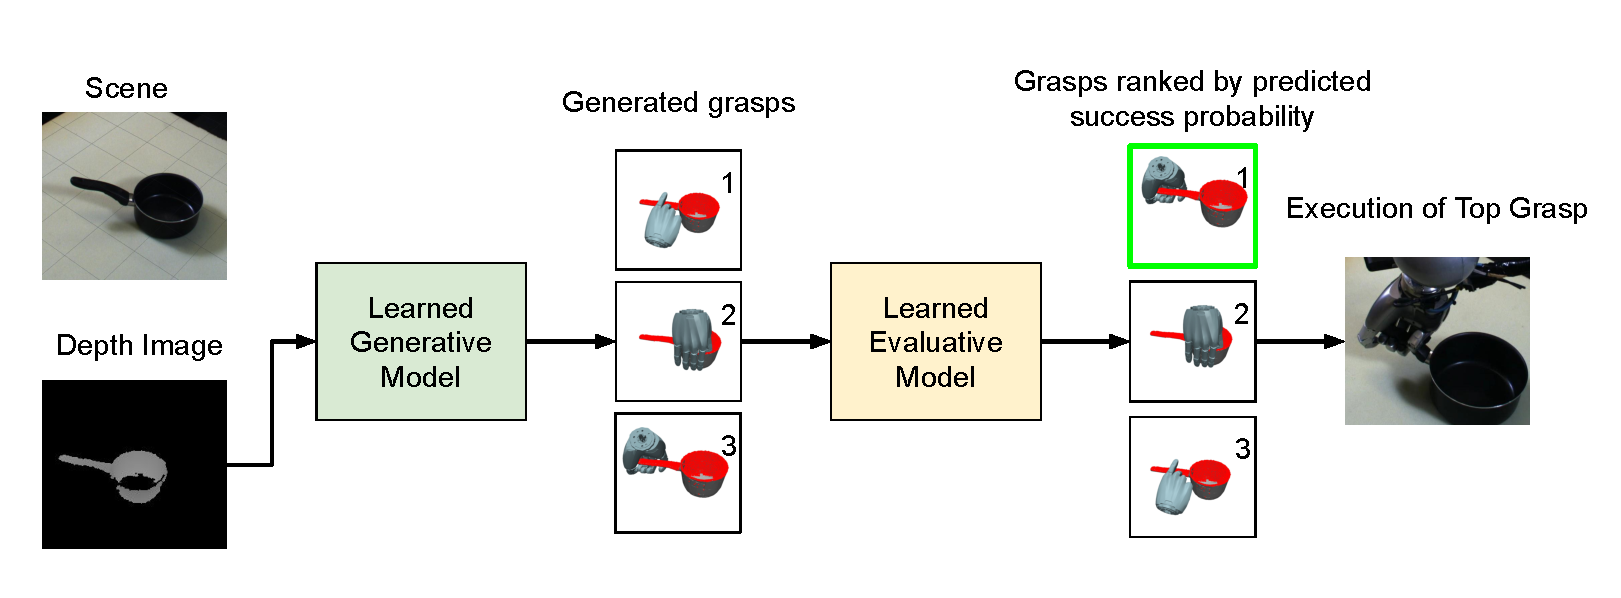
\includegraphics[width=\columnwidth]{images/GEAarchitecture.pdf}
  \end{center}
  \caption{Our grasping architecture. When shown an object, a generative model (GM) produces grasps, ranked according to its likelihood model. These are re-ranked by the predicted success probability of the evaluative Model (EM).The top ranked grasp is executed \label{fig:systemArchitecture}}
\end{figure}

The contributions of this paper are as follows. First, we present a data set of 2.4m simulated dexterous grasps, available to evaluate dexterous grasping algorithms. Second, we release the source code of the dexterous grasp simulator, which can be used to visualise the data set and gather new data.\footnote{The code and simulated grasp data set are available at \href{https://rusen.github.io/DDG}{https://rusen.github.io/DDG}.} Third, we combine an existing learned generative model with multiple learned evaluative models that are trained from simulated grasps proposed by the generative model. Fourth, we present an extensive evaluation of all these models on our simulated data set. Fifth, we compare the two most promising variants on a real robot with a data set of objects in challenging poses. Finally, we perform a deep dive into the simulation results.

The model variants are organised in three dimensions. First, we employ two different generative models (GM1 \cite{kopicki2015ijrr} and GM2 \cite{kopicki2019ijrr}), one of which (GM2) is designed specifically for single view grasping. Second, we use two different back-bones for the evaluative model, VGG-16 and ResNet-50. Third, we experiment with two optimisation techniques--gradient ascent (GA) and stochastic annealing (SA)--to search for better grasps using the evaluative model as an objective function.

%The first contribution of this paper is the first generative-evaluative architecture where both generative and evaluative models are learned. Second, three novel evaluative networks, based on existing VGG-16 and ResNet-50 architectures, were proposed. Finally, a grasp simulation dataset containing 2M+ grasps on 295 objects, along with the simulator code will be released to to the community. In order to simulate the wide range of physical variations that real world objects have, a data set is acquired by simulation of  grasps proposed by the generative models on novel objects. We vary the physical characteristics of the objects in each simulated scene (mass, friction) which the robot can not observe. This dataset was used to train three evaluative neural networks. The evaluative models were then used to rank grasps produced by the generative models (GM1 and GM2) in real robot experiments. 

%The paper builds upon two existing generative grasp models that are learned from a small number of demonstrated grasps using the data-efficient method for LfD. Unlike other approaches to deep grasping, which are restricted to power-grasps, the methods are able to perform a wide variety of grasps, including pinch, rim, power, and handle grasps, and to use additional fingers to provide bracing.

The paper is structured as follows. First, we discuss related work. Second, we describe the design of the grasp simulation, the generation of the data set. Third, the proposed generative evaluative architecture is described and the different architectures employed for the evaluative model are explained, including the optimisation variants of the evaluative model. Fourth, a simulation-based experimental study of the proposed methods is presented. Fifth, we present the real robot study. Finally, we extend the simulation analysis further by examining the inner workings of the best performing model. 


\section{Background and Related Work}

Learning for robot grasping has made steady progress. There are probabilistic machine learning techniques employed for surface estimation for grasping \cite{dragiev2011gaussian}; data efficient methods for learning dexterous grasps from demonstration \cite{ben-amor2012a,kopicki2015ijrr,detry2012a}; logistic regression for classifying grasp features from images \cite{saxena2008a}; and for autonomous learning \cite{detry2010a}. Deep learning is a recent approach to grasping. Most work is for two finger grippers. Approaches either learn an evaluation function for an image-grasp pair \cite{levine16,lenz2015deep,gualtieri2016high,mahler2017dex,pinto2016supersizing,johns2016deep}, learn to predict the grasp parameters \cite{redmon2015real,kumra2017iros} or jointly estimate both \cite{morrison18}. The quantity of real training grasps can be reduced by mixing real and simulated data \cite{bousmalis2017using}. 

A small number of papers have explored deep learning as a method for dexterous grasping. \cite{lu2017planning,varley2015generating,veres2017modeling,zhou20176dof,kappler2015leveraging}. All of these use simulation to generate the training set for learning. Kappler \cite{kappler2015leveraging} showed the ability of a CNN to predict grasp quality for multi-fingered grasps, but uses complete point clouds as object models and only varies the wrist pose for the pre-grasp position, leaving the finger configurations the same. Varley \cite{varley2015generating} and later Zhou \cite{zhou20176dof} went beyond this, each being able to vary the hand pre-shape, and predicting from a single image of the scene. Each of these posed search for the grasp as a pure optimisation problem (using simulated annealing or quasi-Newton methods) on the output of the CNN. They all, also, take the approach of learning an evaluative model, and generate candidates for evaluation uninfluenced by prior knowledge. Veres \cite{veres2017modeling}, in contrast, learns a deep generative model. Finally Lu \cite{lu2017planning} learns an evaluative model, and then, given an input image, optimises the inputs that describe the wrist pose and hand pre-shape to this model via gradient descent, but does not learn a generative model. In addition, the grasps start with a heuristic grasp which is varied within a limited envelope. Of the papers on dexterous grasp learning with deep networks only two approaches \cite{varley2015generating,lu2017planning} have been tested on real grasps, with eight and five test objects each, producing success rates of 75\% and 84\% respectively. An important restriction of both of these methods is that they only plan the pre-grasp, not the finger-surface contacts and are thus limited to power-grasps.

Thus, in each case, either an evaluative model is learned but there is no learned prior over the grasp configuration able to employed as a generative model; or a generative grasp model is learned, but there is no evaluative model learned to select the grasp. Our novelty is thus to bring together a data-efficient method of learning a good generative model with an evaluative model. As with others, we learn the evaluative model from simulation, but the generative model is learned from a small number of demonstrated grasps. 


%n learning to grasp divides into two categories, that we label {\em generative} and {\em evaluative} respectively. We quickly summarise the relationship between this paper and these two.
%
%Generative approaches to grasping include the work of detry et al, kopicki et al, these methods learn distributions of grasps from positive examples. In the case of detry, saxena, these are pinch grasps that are associated with features extracted from monocular or stereo images. Both those pieces of work were restricted to pinch grasps. Both Saxena and Detry require significant training samples, but Detry used real grasps, whereas Saxena used simulation to generate training exemplars. Other approaches use LfD rather than autonomous exploration, as this can significantly reduce the training data required. Peters et al introduced a method for generative grasping by grasp warping, demonstrating an ability to handle new objects of a similar global shape to the training objects. Kopicki et al introduced a factored generative model, showing grasp transfer to novel objects from one example of each grasp type. This is the method than we replicate and build on in our work.
%
%Evaluative approaches to grasping include the work of levine, in which a farm of fourteen robot were used over a two month data gathering period. This data is used to train a neural network that predicts the probability of success of a pinch grasp conditional on an image. In that work the only input is an RGB image, but other approaches to deep grasping tenpas use depth images. However, all these approaches are all data intensive. 
%
%The work that is closest to ours, and the only paper of which we are aware on deep learning applied to dexterous grasping, is that of Hermans et al. 

\section{The Simulated Grasp Data Set}
\label{section:simulation}j
%Introductory sentences here
In this section, we describe how we generated a realistic simulated data set for dexterous grasping. This captures variations in both observable (e.g. object pose) and unobservable (e.g. surface friction) parameters.

To generate the training set a simulated depth image of a scene containing a single unfamiliar object is generated. Using either of the generative models GM1 or GM2, grasps are generated and executed in simulation. The success or failure of each simulated grasp is recorded. Producing a good simulation for evaluating grasps is non-trivial. An important problem is that the data set must capture the natural uncertainty in unobservable variables, such as mass and friction. Since many of these parameters are unobservable we are thus creating a data set such that the grasp policy must work across a range of variations. This is thus a form of {\em domain randomisation}. A similar technique has been employed by \cite{mahler2017dex}, but we extend it from a single grasp quality metric to full rigid body simulation.

\subsection{Features and Constraints of the Virtual Environment}
\label{subsection:environment}

The collected 3D model dataset contains 294 objects from 20 classes, namely, bottles, bowls, cans, boxes, cups, mugs, pans, salt and pepper shakers, plates, forks, spoons, spatulas, knives, teapots, teacups, tennis balls, dustpans, scissors, funnels and jugs (Figure \ref{fig:allObjects}). All objects in the dataset can be grasped using the DLR-II hand, although there are limitations on how some object classes can be approached. For example, teapots and jugs are not easy to grasp except by their handles due being larger than the hand's maximum aperture, while small objects such as salt and pepper shakers can be approached in more creative ways. The number of objects in each class varies from 1 (dustpan) to 25 (bottles). Long/thin objects such as kitchen utensils are placed vertically in a short, heavy stand in order to make them graspable without touching the table. This reflects the real-world scenario, as attempting to grasp a spatula lying on a table would be dangerous for the robotic hand. In total, 250 objects from all 20 classes were allocated for training and validation, while the remaining 44 objects from 19 classes belong to the test set.

We employ MuJoCo \cite{MuJoCo} as the rigid-body simulator. Due to the fact that collision checking in MuJoCo requires that objects comprise convex parts, all 294 objects were decomposed into convex parts using V-HACD algorithm \cite{V-HACD}. The number of sub-parts varies from 2 to 120.

During the scene creation, the object is placed on the virtual table at a pseudo-random pose. Most objects are placed in a canonical upright pose, and only randomly rotated around the gravity axis (akin to being placed on a turntable). The objects belonging to the mug and cup classes have fully random 3D rotations applied before they are placed on the table, since it is possible to grasp them in almost any setting using the robot hand.

\begin{figure}
  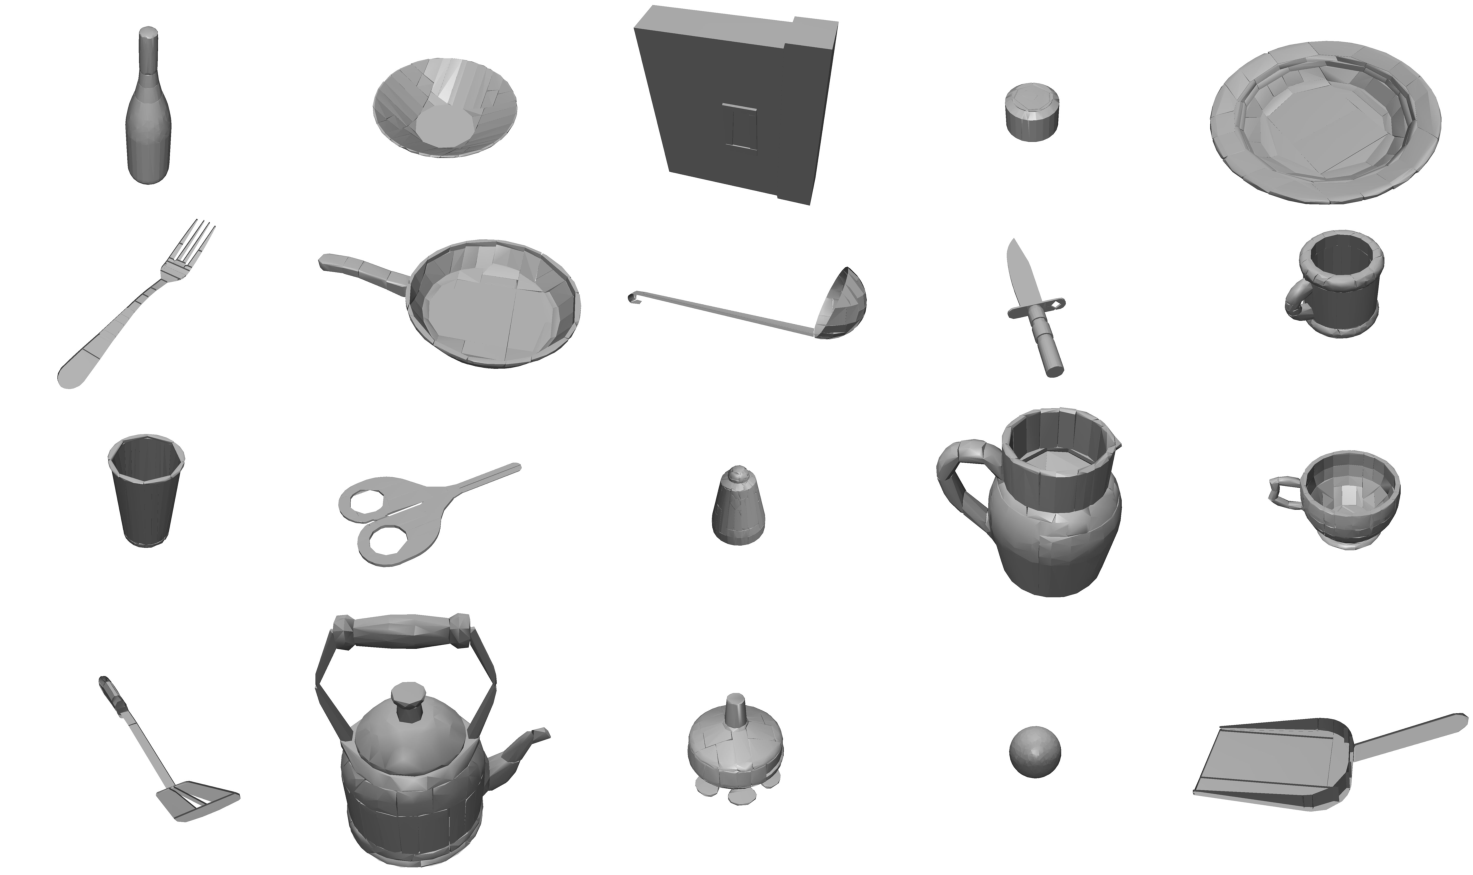
\includegraphics[width=\linewidth]{images/allObjects-small.pdf}
  \caption{A sample of the 294 objects drawn from the 20 object classes.
  \label{fig:allObjects}}
\end{figure}

To achieve domain randomisation, prior distributions for mass, size and frictional coefficient were estimated from real-world data. The properties of simulated objects are sampled from these priors. For each object its mean size, mass and friction coefficient are matched to a real counterpart. For each trial, the size is randomly scaled by a factor in the range [0.9,1.1], while remaining within the grasp aperture of the hand. Object mass is uniformly sampled from a category specific range, estimated from real objects (Table~\ref{fig:weights}). The friction coefficient of each object is sampled from a range of $[0.5, 1]$ in MuJoCo default units, intended to simulate surfaces from low-friction (metal) to high-friction (rubber). This variation is critical to ensuring that the evaluative model will predict the robustness of a grasp to unobservable variations.
\begin{table}[]
\centering
\caption{Mass ranges for each object class (grams).}
\label{fig:weights}
\resizebox{\linewidth}{!}{\begin{tabular}{|l|l|l|l|l|l|l|}
\hline
Bottle & Bowl     & Box     & Can     & Cup    & Fork    & Pan     \\ \hline
30-70  & 50-400   & 50-500  & 200-400 & 30-330 & 40-80   & 150-450 \\ \hline
Plate  & Scissors & Shaker  & Spatula & Spoon  & Teacup  & Teapot  \\ \hline
40-80  & 50-150   & 100-160 & 40-80   & 40-80  & 150-250 & 500-800 \\ \hline
Jug    & Knife    & Mug     & Funnel  & Ball   & Dustpan &         \\ \hline
80-200 & 50-150   & 250-350 & 40-80   & 50-70  & 100-150 &         \\ \hline
\end{tabular}}
\end{table}
 
For depth image simulation the Carmine 1.09 depth sensor installed on the robot is simulated with a modified version of the Blensor Kinect sensor simulator \cite{KinectSimulator}. For each object, we vary the camera orientation and distance from the object, as well as object mass, friction, scale, location and orientation. In order to account for calibration errors in the real world setup, we add a small three-dimensional positional noise to each point in the sensor output.

A 3D mesh-model of the DLR-II hand has been used in the simulator. There are no kinematic constraints on how the hand may grasp an object, other than collisions with the table. To ensure realism, we use impedance control for the hand.
%The reasons for the most critical of these decisions are now given in slightly more detail. First, in order to create a realistic simulation environment, we chose the MuJoCo \cite{MuJoCo} physics simulator over other simulators (OpenSim, BulletPhysics, ODE, NVIDIA PhysX) for two reasons: 
%\begin{itemize}
%\item MuJoCo uses generalized coordinates and optimization-based contact dynamics, resulting in fewer numerical instabilities,
%\item MuJoCo is optimized for the quality of physics as well as its speed, hence improving the quality of the physics simulation.
%\end{itemize}
\begin{figure}
  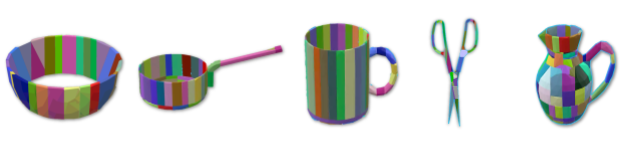
\includegraphics[width=\linewidth]{images/decomposition.png}
  \caption{Approximate convex decomposition of some objects in our dataset. Best viewed in colour.}
  \label{fig:objectDecomposition}
\end{figure}

Some classes are easier to grasp than others. Table \ref{fig:graspperf} shows the success rates of the generated grasps in each class, when attempted with the grasps ranked by the Generative Model (GM1). The sampled grasps perform well on a number of classes including Dustpans, Scissors, Spoons, and Mugs. Some objects can only be grasped in certain ways, i.e. not all 10 training grasps are applicable to all objects.

\begin{table}[]
\centering
\caption{The average and \textbf{top} grasp success rates of GM1 on simulated data.}
\label{fig:graspperf}
\resizebox{\linewidth}{!}{\begin{tabular}{|l|l|l|l|l|l|l|}
\hline
Bottle & Bowl     & Box     & Can     & Cup    & Fork    & Pan     \\ \hline
35.5 - \textbf{47.7}\% & 26.4 - \textbf{61.2}\%   & 16.5 - \textbf{30.1}\%  & 41.4 - \textbf{92.6}\% & 44.7 - \textbf{59.9}\% & 59.6 - \textbf{68.1}\%   & 37.9 - \textbf{57.3}\% \\ \hline
Plate  & Scissors & Shaker  & Spatula & Spoon  & Teacup  & Teapot  \\ \hline
50.2 - \textbf{95.5}\%  & 62.7 - \textbf{69.9}\%   & 47.3 - \textbf{53.3}\% & 57.4 - \textbf{65.7}\%   & 63.4 - \textbf{82.4}\%  & 48.2 - \textbf{91.2}\% & 26.9 - \textbf{23.9}\% \\ \hline
Jug    & Knife    & Mug     & Funnel  & Ball   & Dustpan & \textbf{Total}      \\ \hline
24.9 - \textbf{43.9}\% & 58.3 - \textbf{65.0}\%   & 40.7 - \textbf{80.9}\% & 52.3 - \textbf{65.9}\%   & 28.0 - \textbf{82.8}\%  & 60.1 - \textbf{78.8}\% & 45.8 - \textbf{63.2}\%        \\ \hline
\end{tabular}}
\end{table}

\subsection{Data Collection Methodology}
\label{subsection:dataCollection}

The data set is divided into units called \textit{scenes}, where each scene comprises a single object placed on a table. This object has a specific set of physical parameters, chosen as described below. Many views and grasps are attempted per scene. Below, we specify the time flow of data collection:

\begin{enumerate}
\item A novel instance of an object from the dataset is generated and placed on a virtual table. Variations are applied to object pose, scale, mass, and friction coefficients.
\item A simulated camera takes a depth image $I_s$ of the scene, converted to a point cloud $P_s$. The viewpoint ${elevation}_s$ of the view point is from 30-57 degrees. The ${azimuth}_s$ is sampled from $[0, 2\pi]$. 
\item The positions of all points in the point cloud $P_s$ are shifted by a three-dimensional noise vector sampled from a Gaussian distribution with parameters $\mu=0$ and $\sigma = 0.004$ (unit: meter).
\item Given $P_s$, the chosen generative model (GM1 or GM2) proposes the candidate grasps. For GM1, up to100 grasps are selected. These are the 10 grasps that are highest ranked by the GM for each of the 10 training grasps. For GM2, we select a maximum of 500 grasps: up to 50 grasps from each training grasp.
\item The grasps are applied to the object in simulation.
\item 19 further simulated depth images are taken from other viewpoints around the object, as explained in step 2. Images with fewer than 250 depth points are discarded. We then sample with replacement from the remaining images and associate each sampled image and viewpoint with a grasp created in step 3.
\item The grasp outcome, trajectory and depth image are stored for each trial. The grasp parameters are converted to the camera frame for the associated view.
\end{enumerate}

%Each candidate grasp $h_i = \{w_0, ..., w_{n}\}$ consists of a series of 10 waypoints along : $w_0$, ..., $w_{n}$. A waypoint $w_k$ is a 27-element vector that specifies full configuration of the hand in joint space: 3 dimensions for 3D coordinates and 4 dimensions for the orientation of the wrist, and 20 parameters specifying each finger joint's activation. 
%After a grasp $h_i$ is generated in world coordinates, the waypoints that belong to the grasp are converted to the camera's frame of reference. 
%The goal of our network architecture is to learn which grasps are more likely to succeed given a point cloud, where both input channels are represented in terms of the camera frame of reference. %This point differentiates us from the work of Levine et al. \cite{Levine1}, where camera coordinates are not used. It should be noted that the possible camera locations in our simulated data covers a larger space, with full circular movement $[0, 2\pi]$ on azimuth and $[30-57]$ range in elevation. Our scenes do not have any distinguishing landmarks such as a bin or robot base, which may aid the network in locating the camera in the scene. 

In each scene $S_i$, a number of depth images are taken $\{I_{ik}\}_{k=0}^{20}$, in the manner explained above. The first image $I_{i0}$ is used to generate grasps, as explained in Section \ref{section:generative}. We typically perform 10-500 grasps per scene. Attaching different views to each grasp instead of the seed image $I_{i0}$ ensures there is more variation in terms of viewpoints, resulting in a richer dataset. Typically, performing a grasp takes half the time it takes to acquire an image using the simulated camera.

Once a grasp is performed in simulation, it is considered a success if an object is lifted one metre above the table, and held there for two seconds. If the object slips from the hand during lifting or holding, the grasp is a failure. 

\begin{figure}[t]
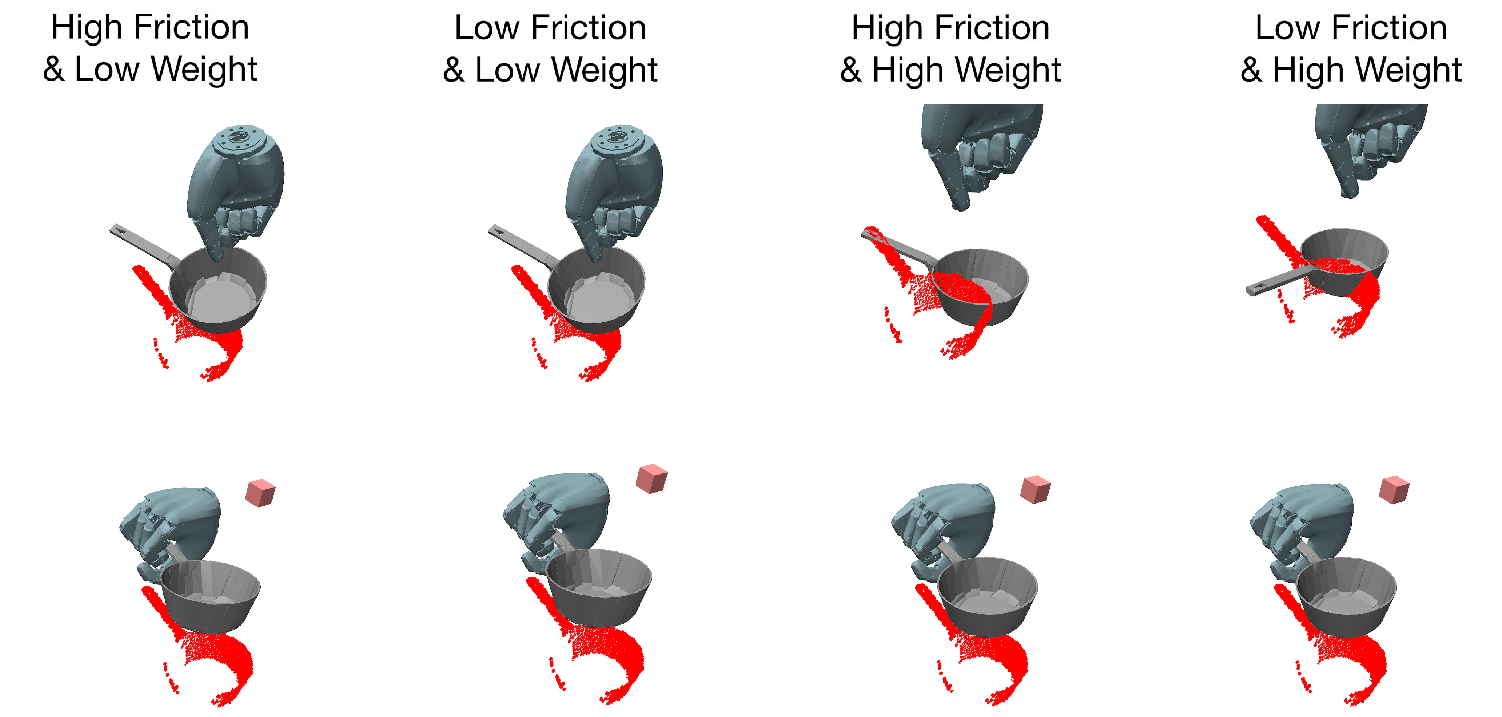
\includegraphics[width=\columnwidth]{images/frictionweight}
%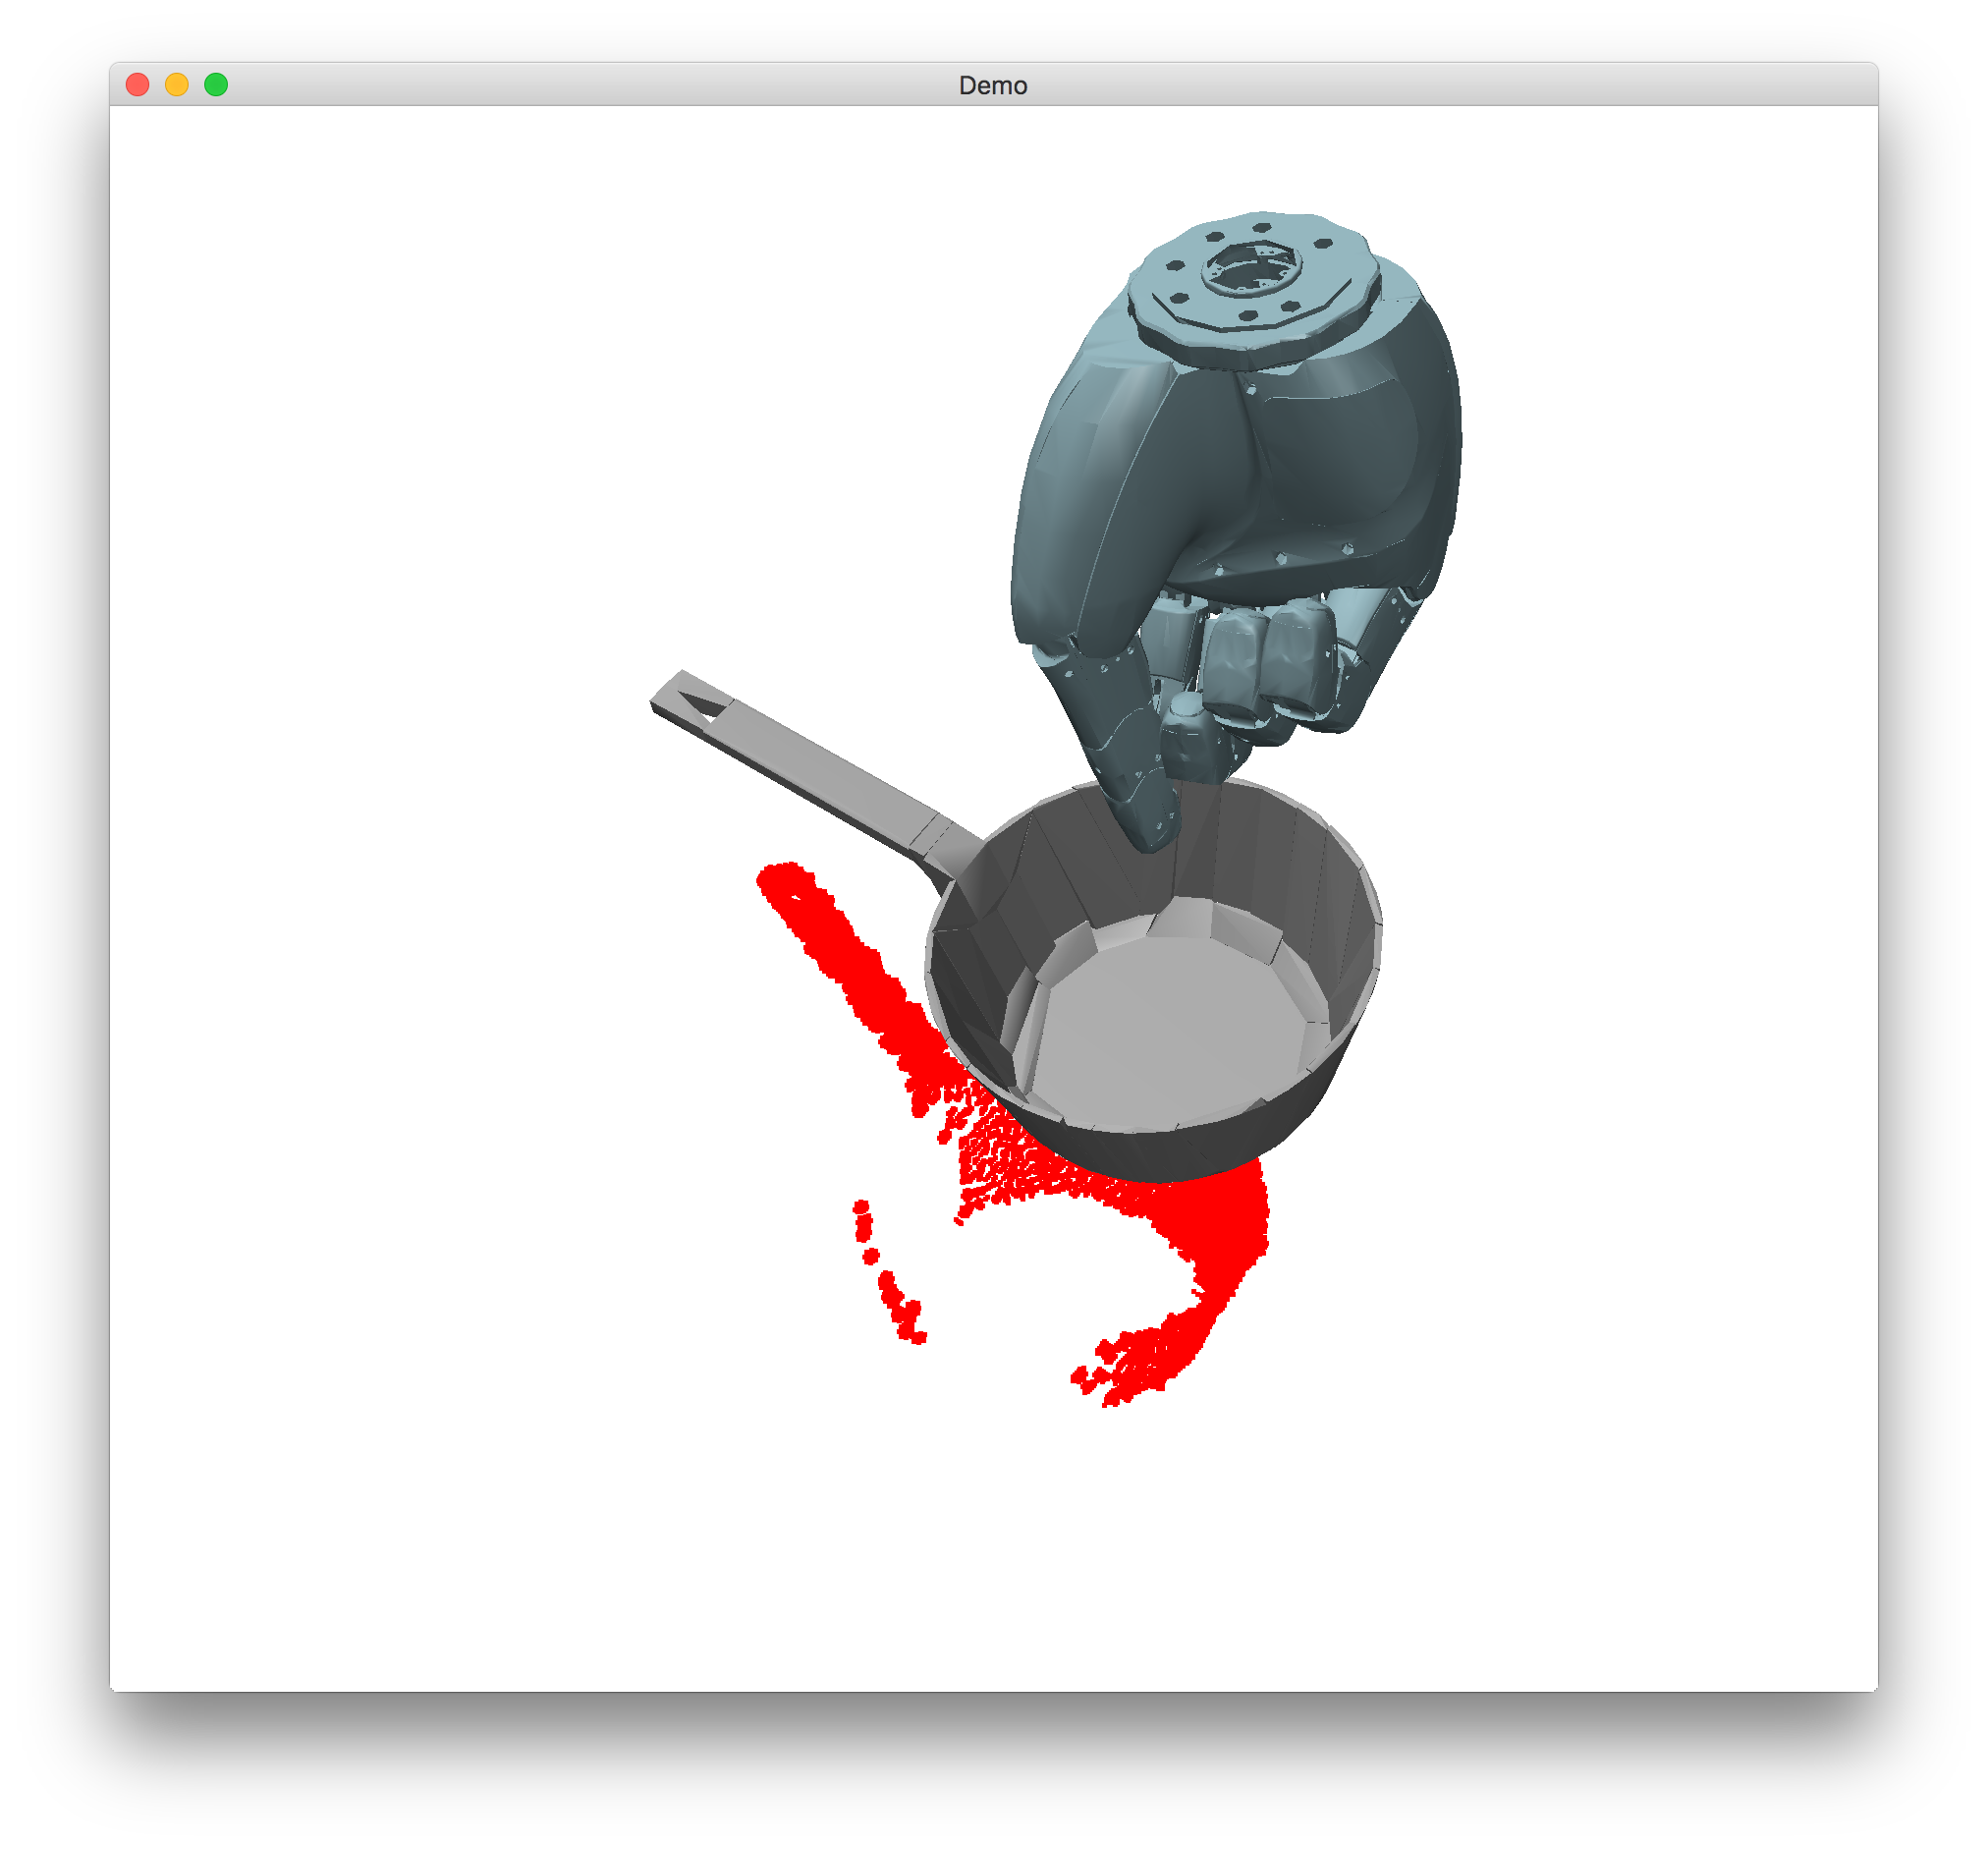
\includegraphics[width=0.24\textwidth]{images/Pan4_2_HFLW}
%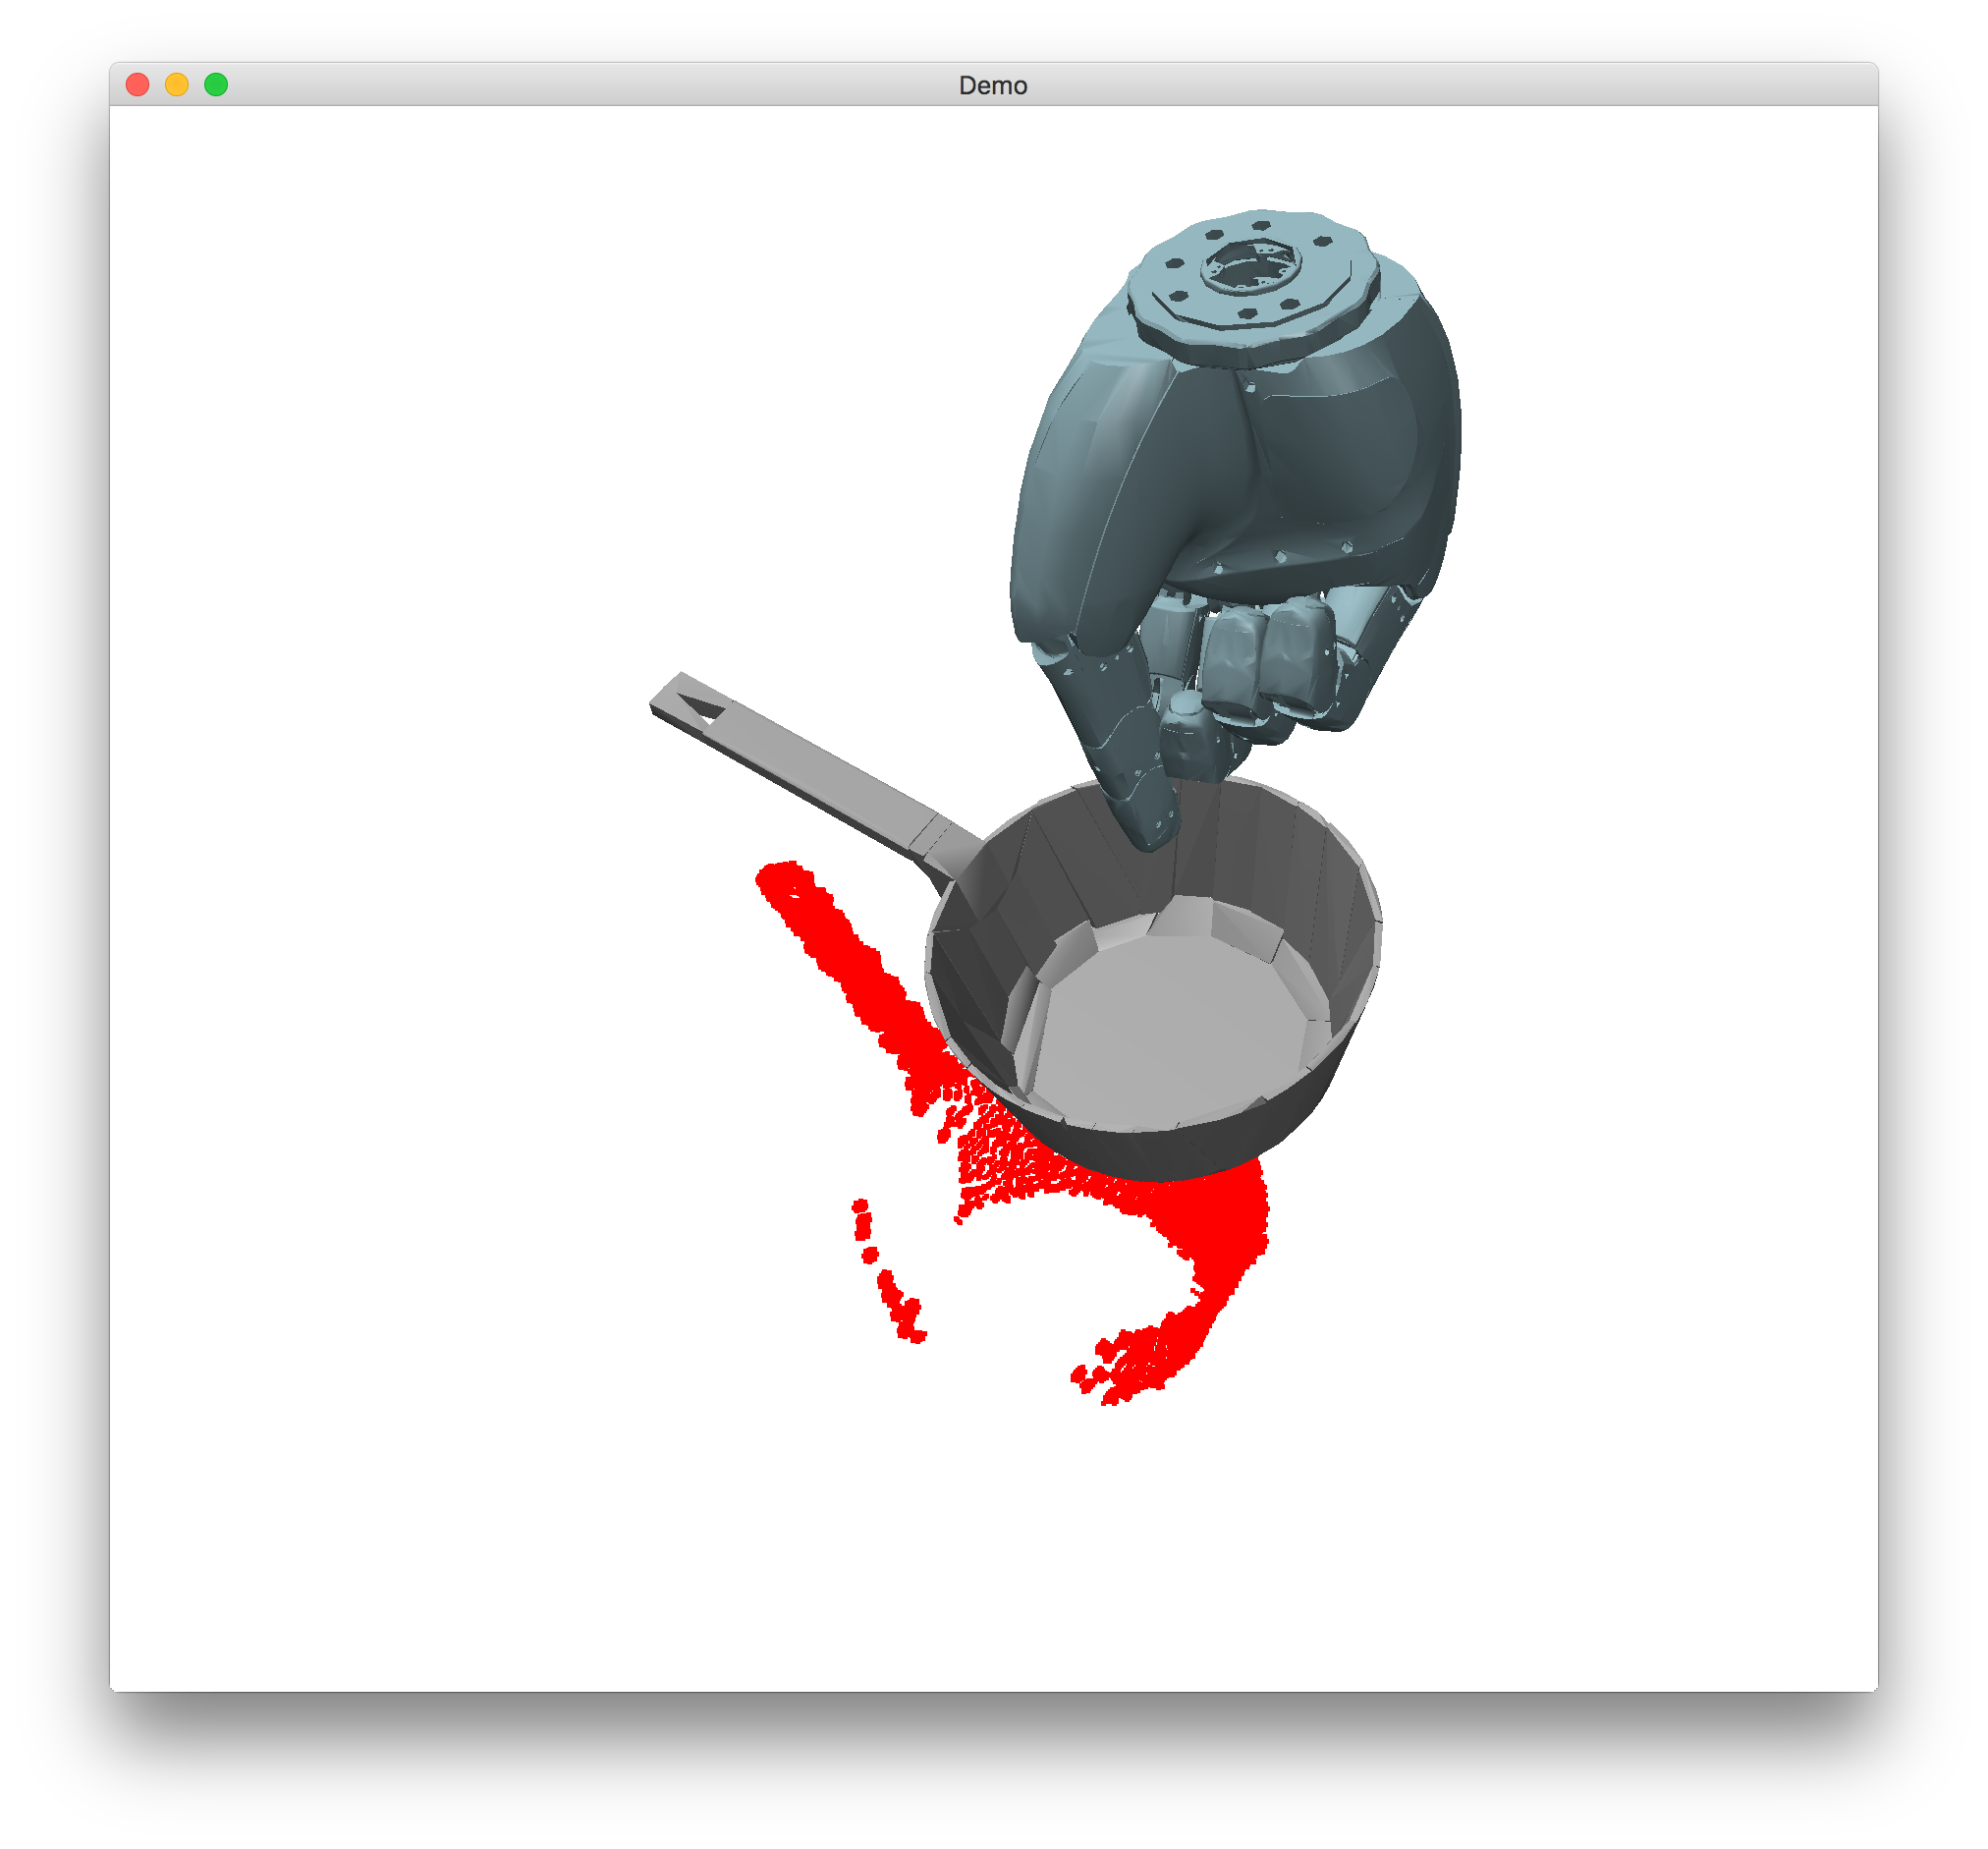
\includegraphics[width=0.24\textwidth]{images/Pan4_2_LFLW}
%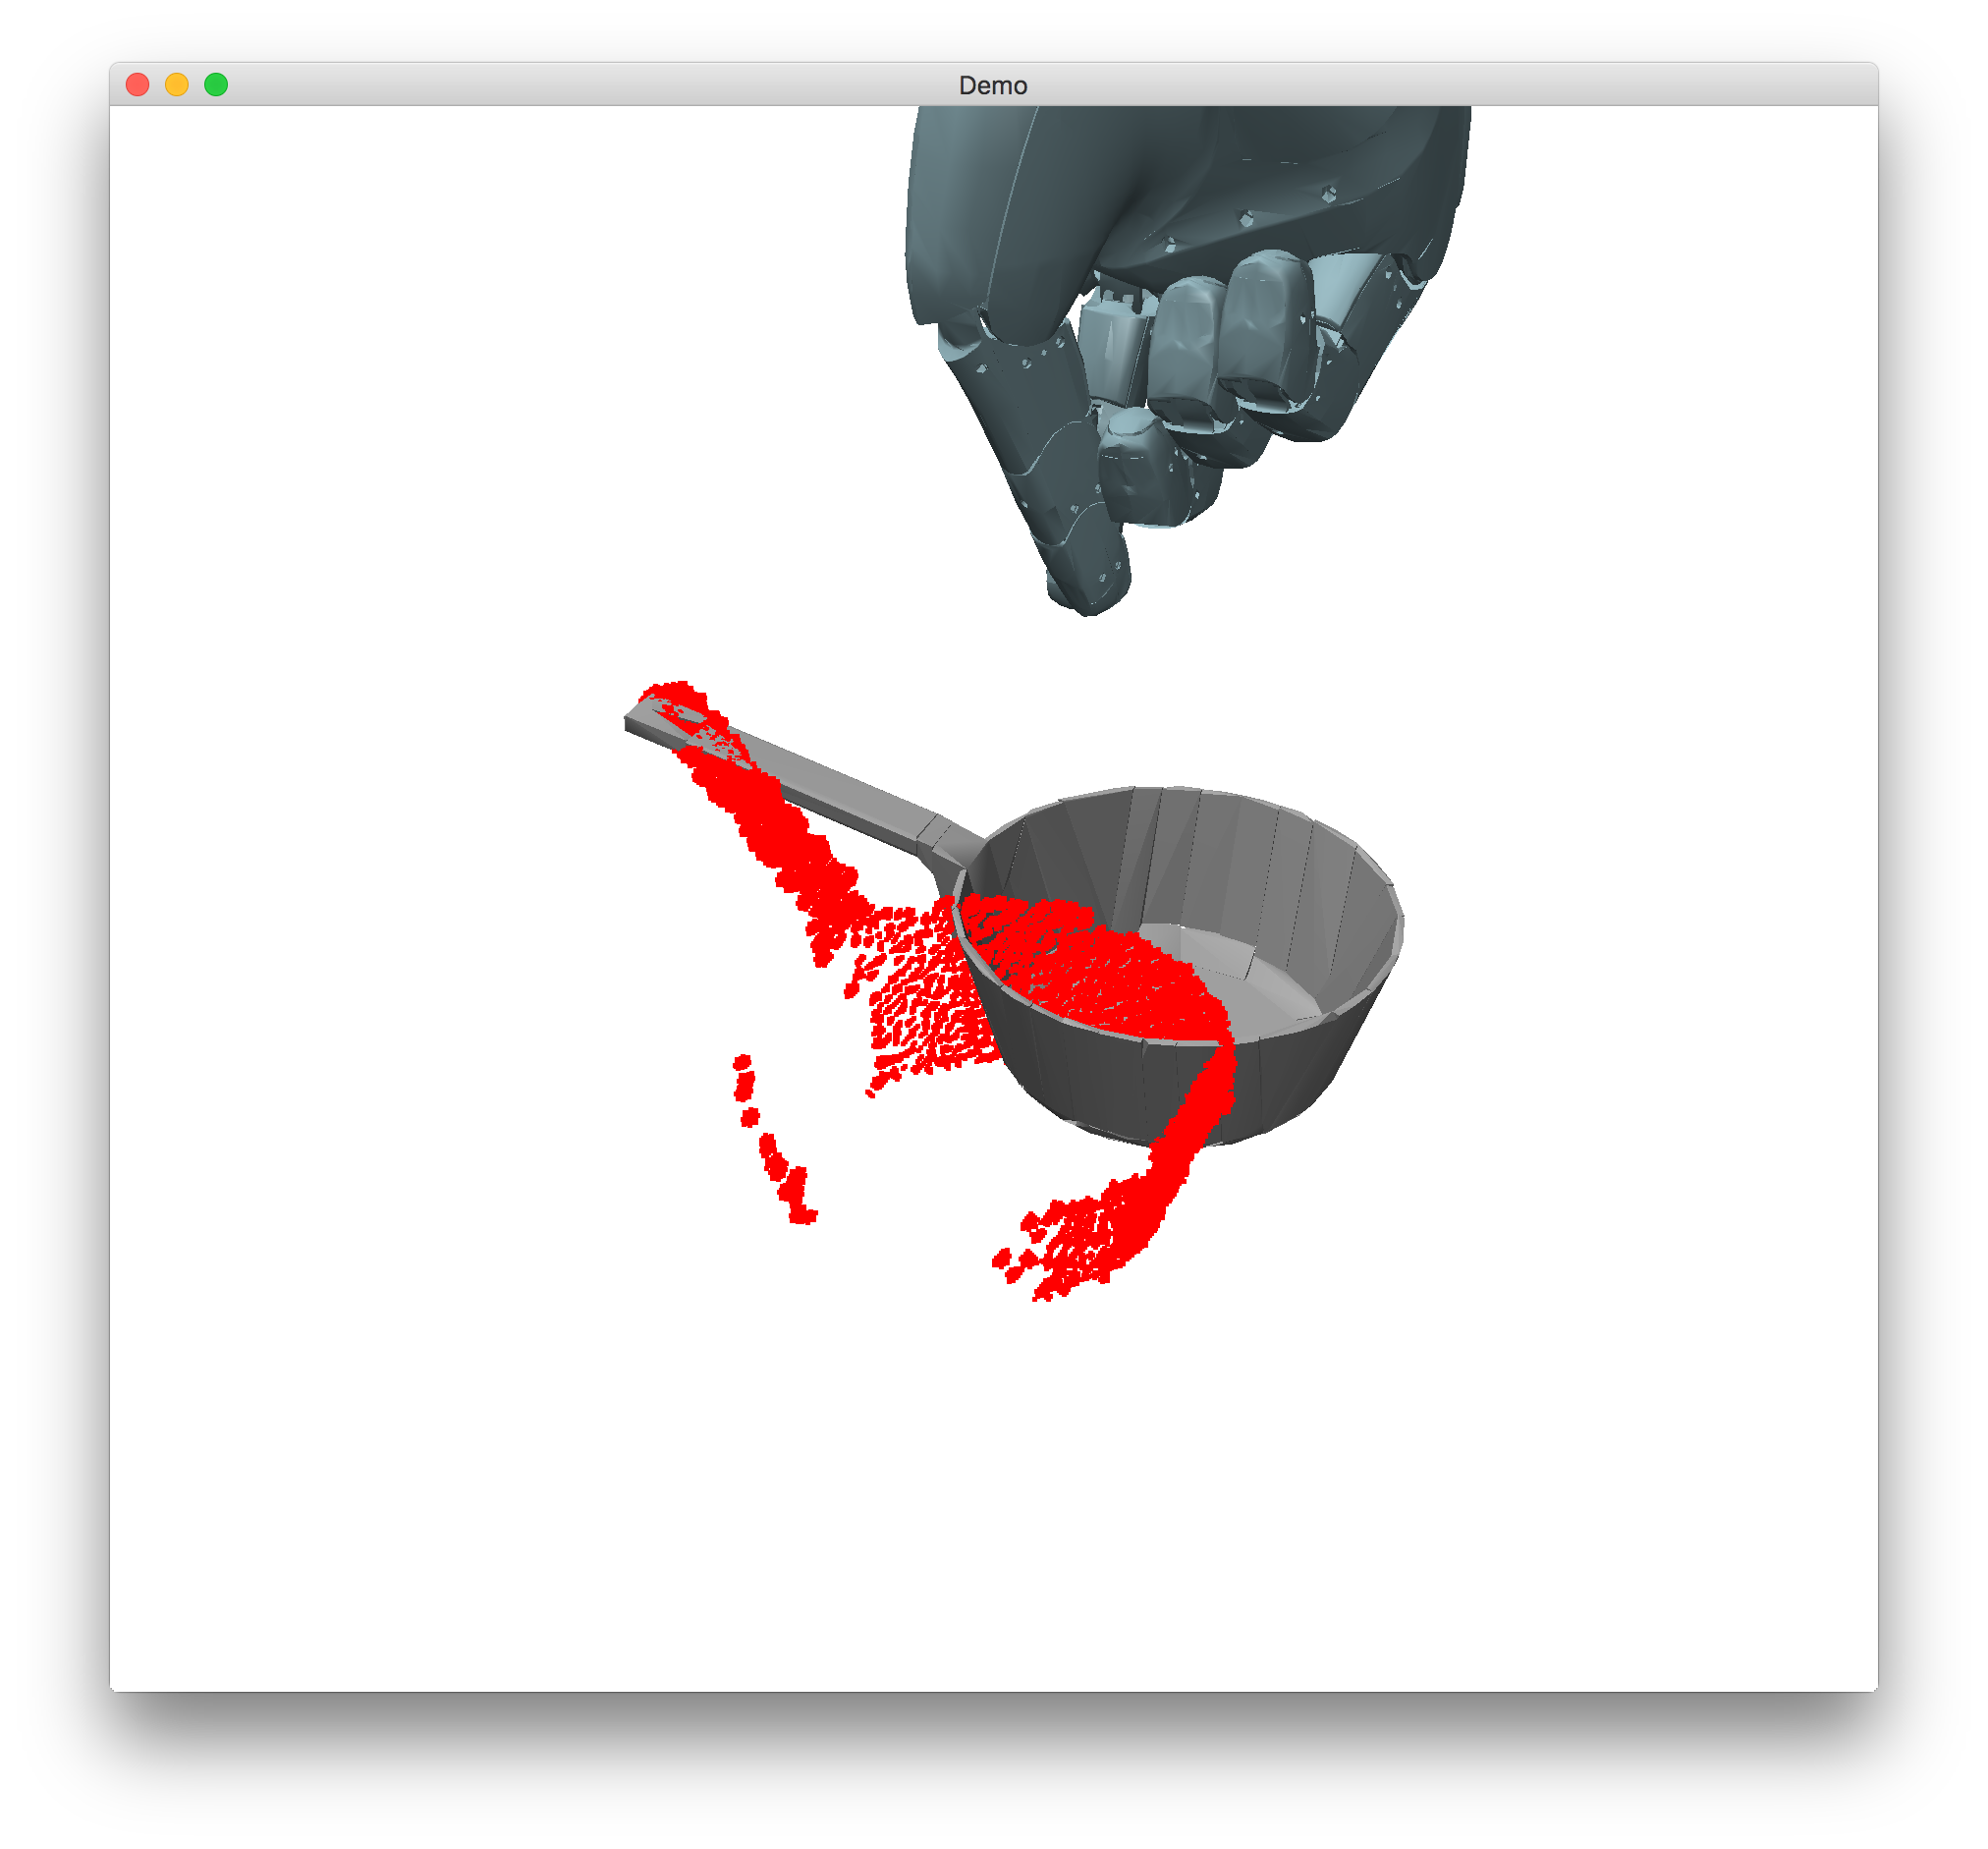
\includegraphics[width=0.24\textwidth]{images/Pan4_2_HFHW}
%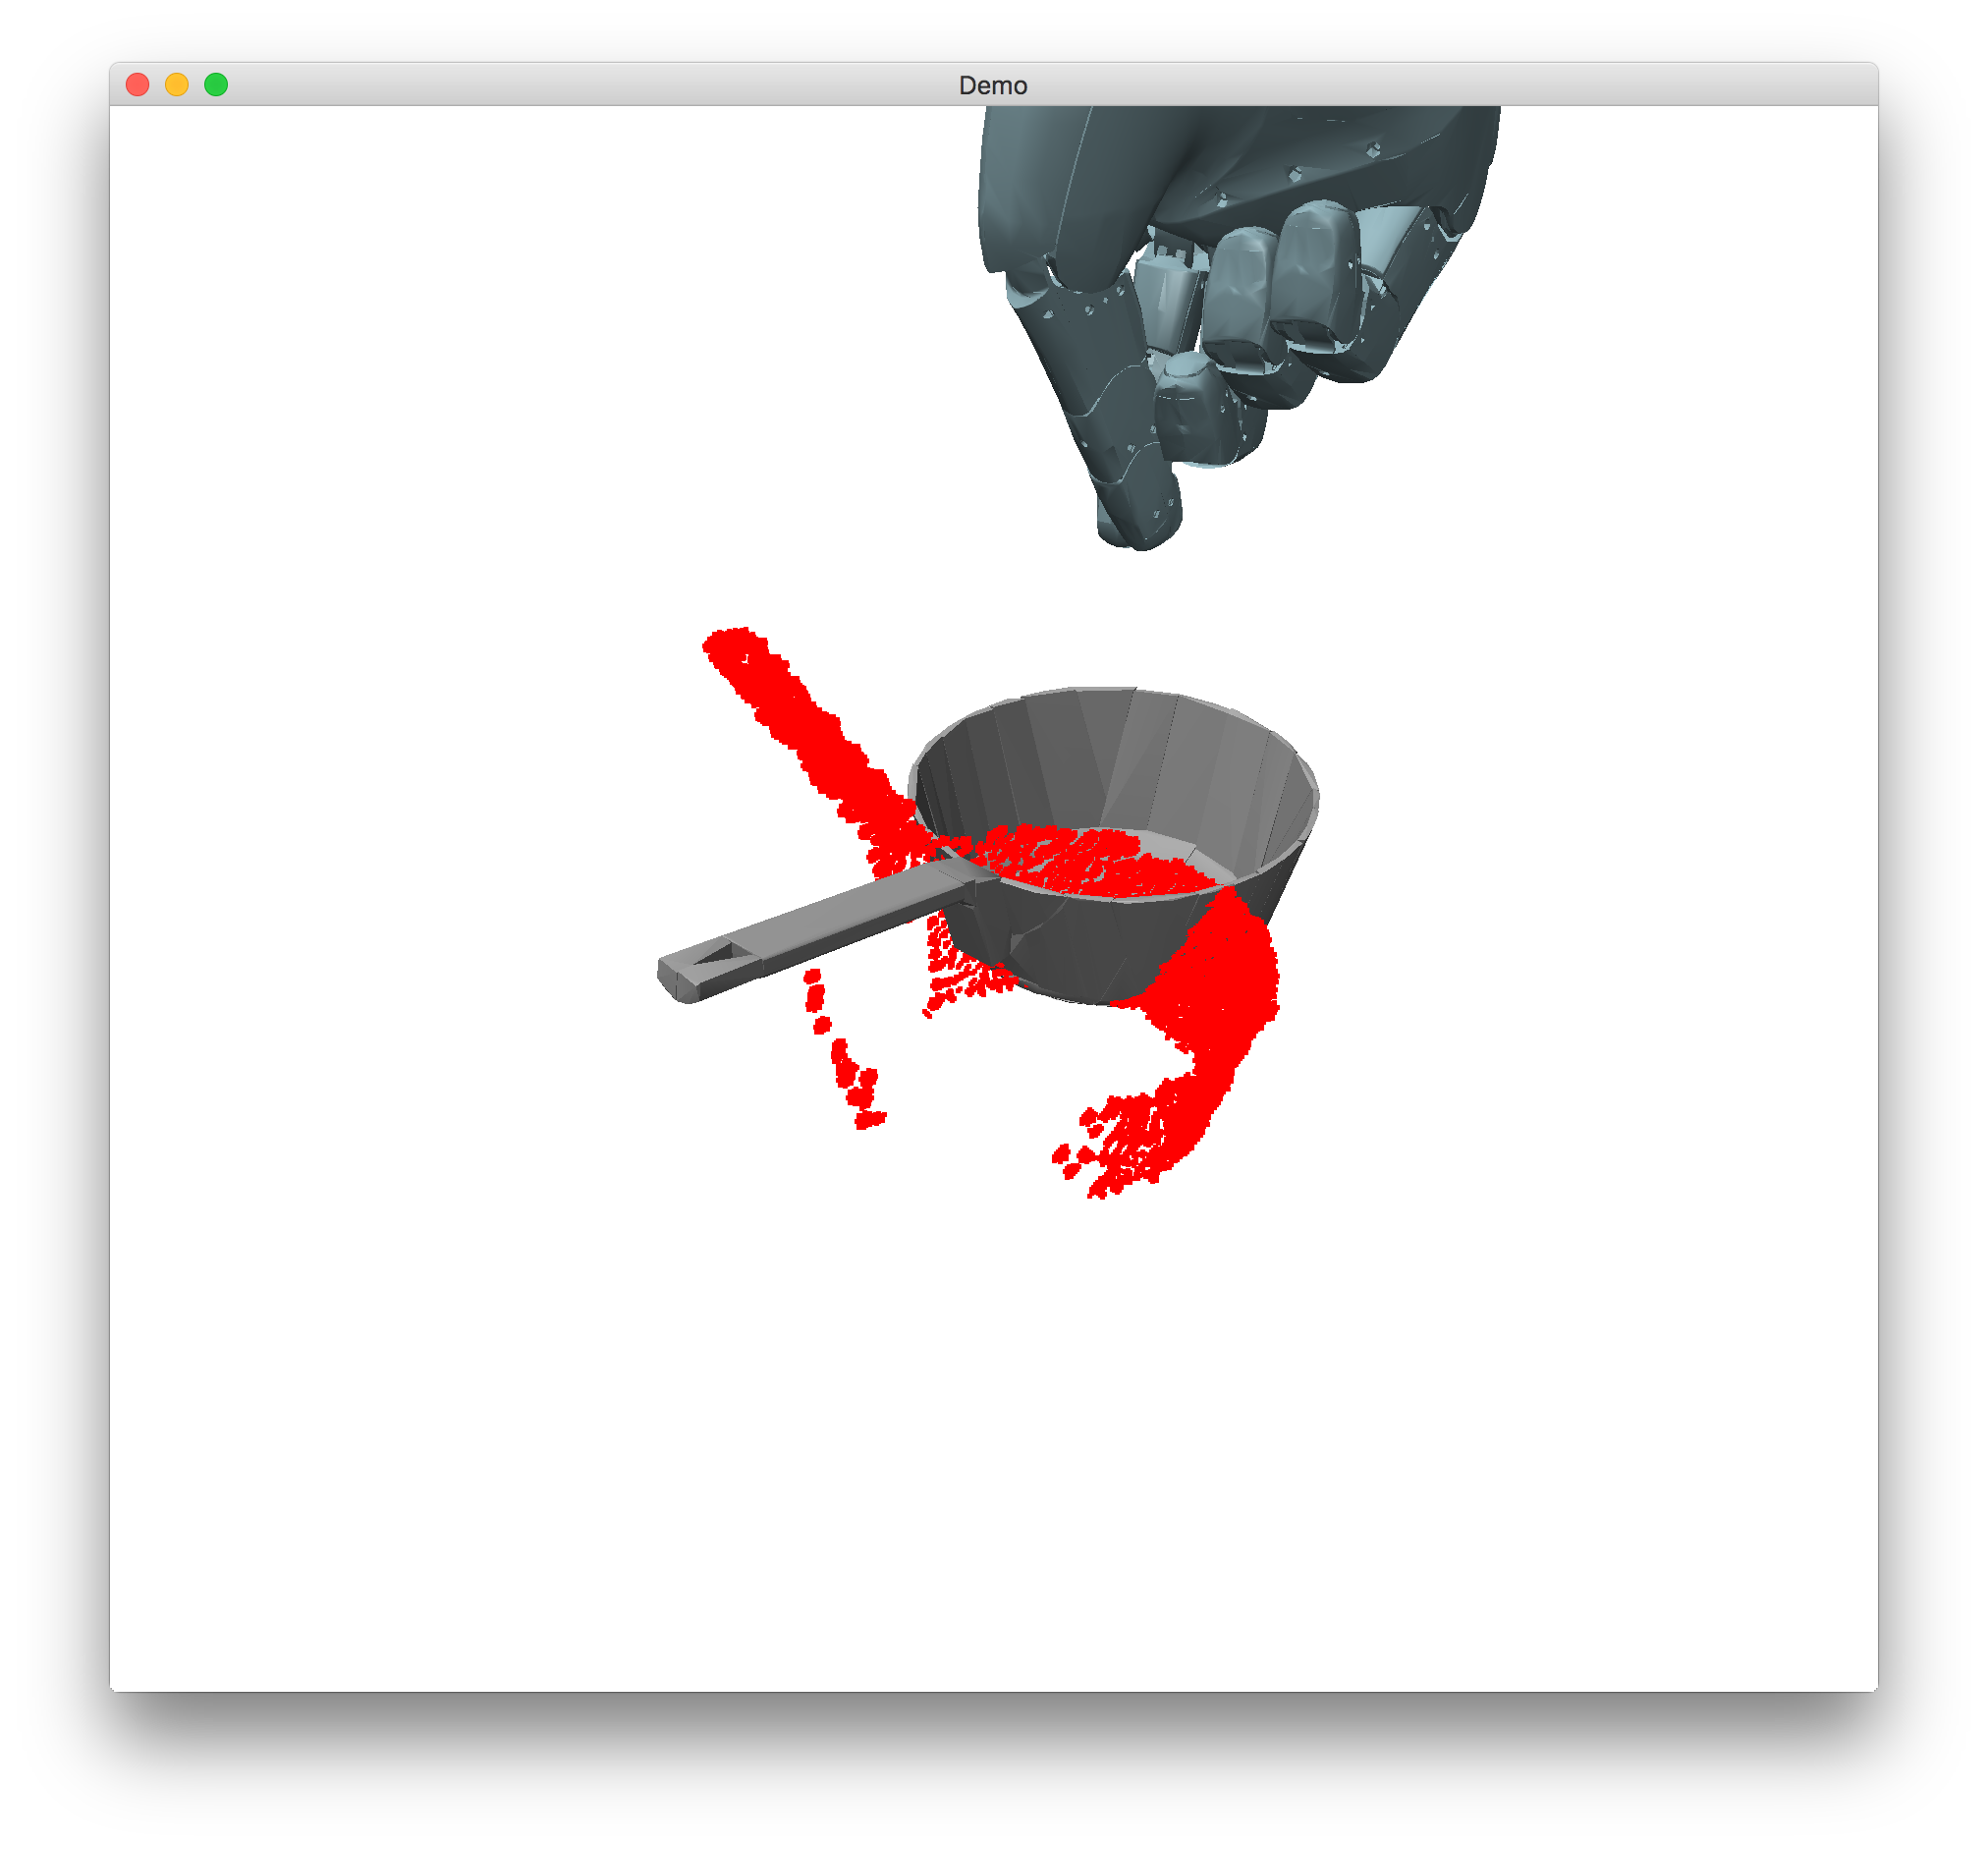
\includegraphics[width=0.24\textwidth]{images/Pan4_2_LFHW}\\
%%
\includegraphics[width=0.96\textwidth]{images/key-to-eval-training}\\
%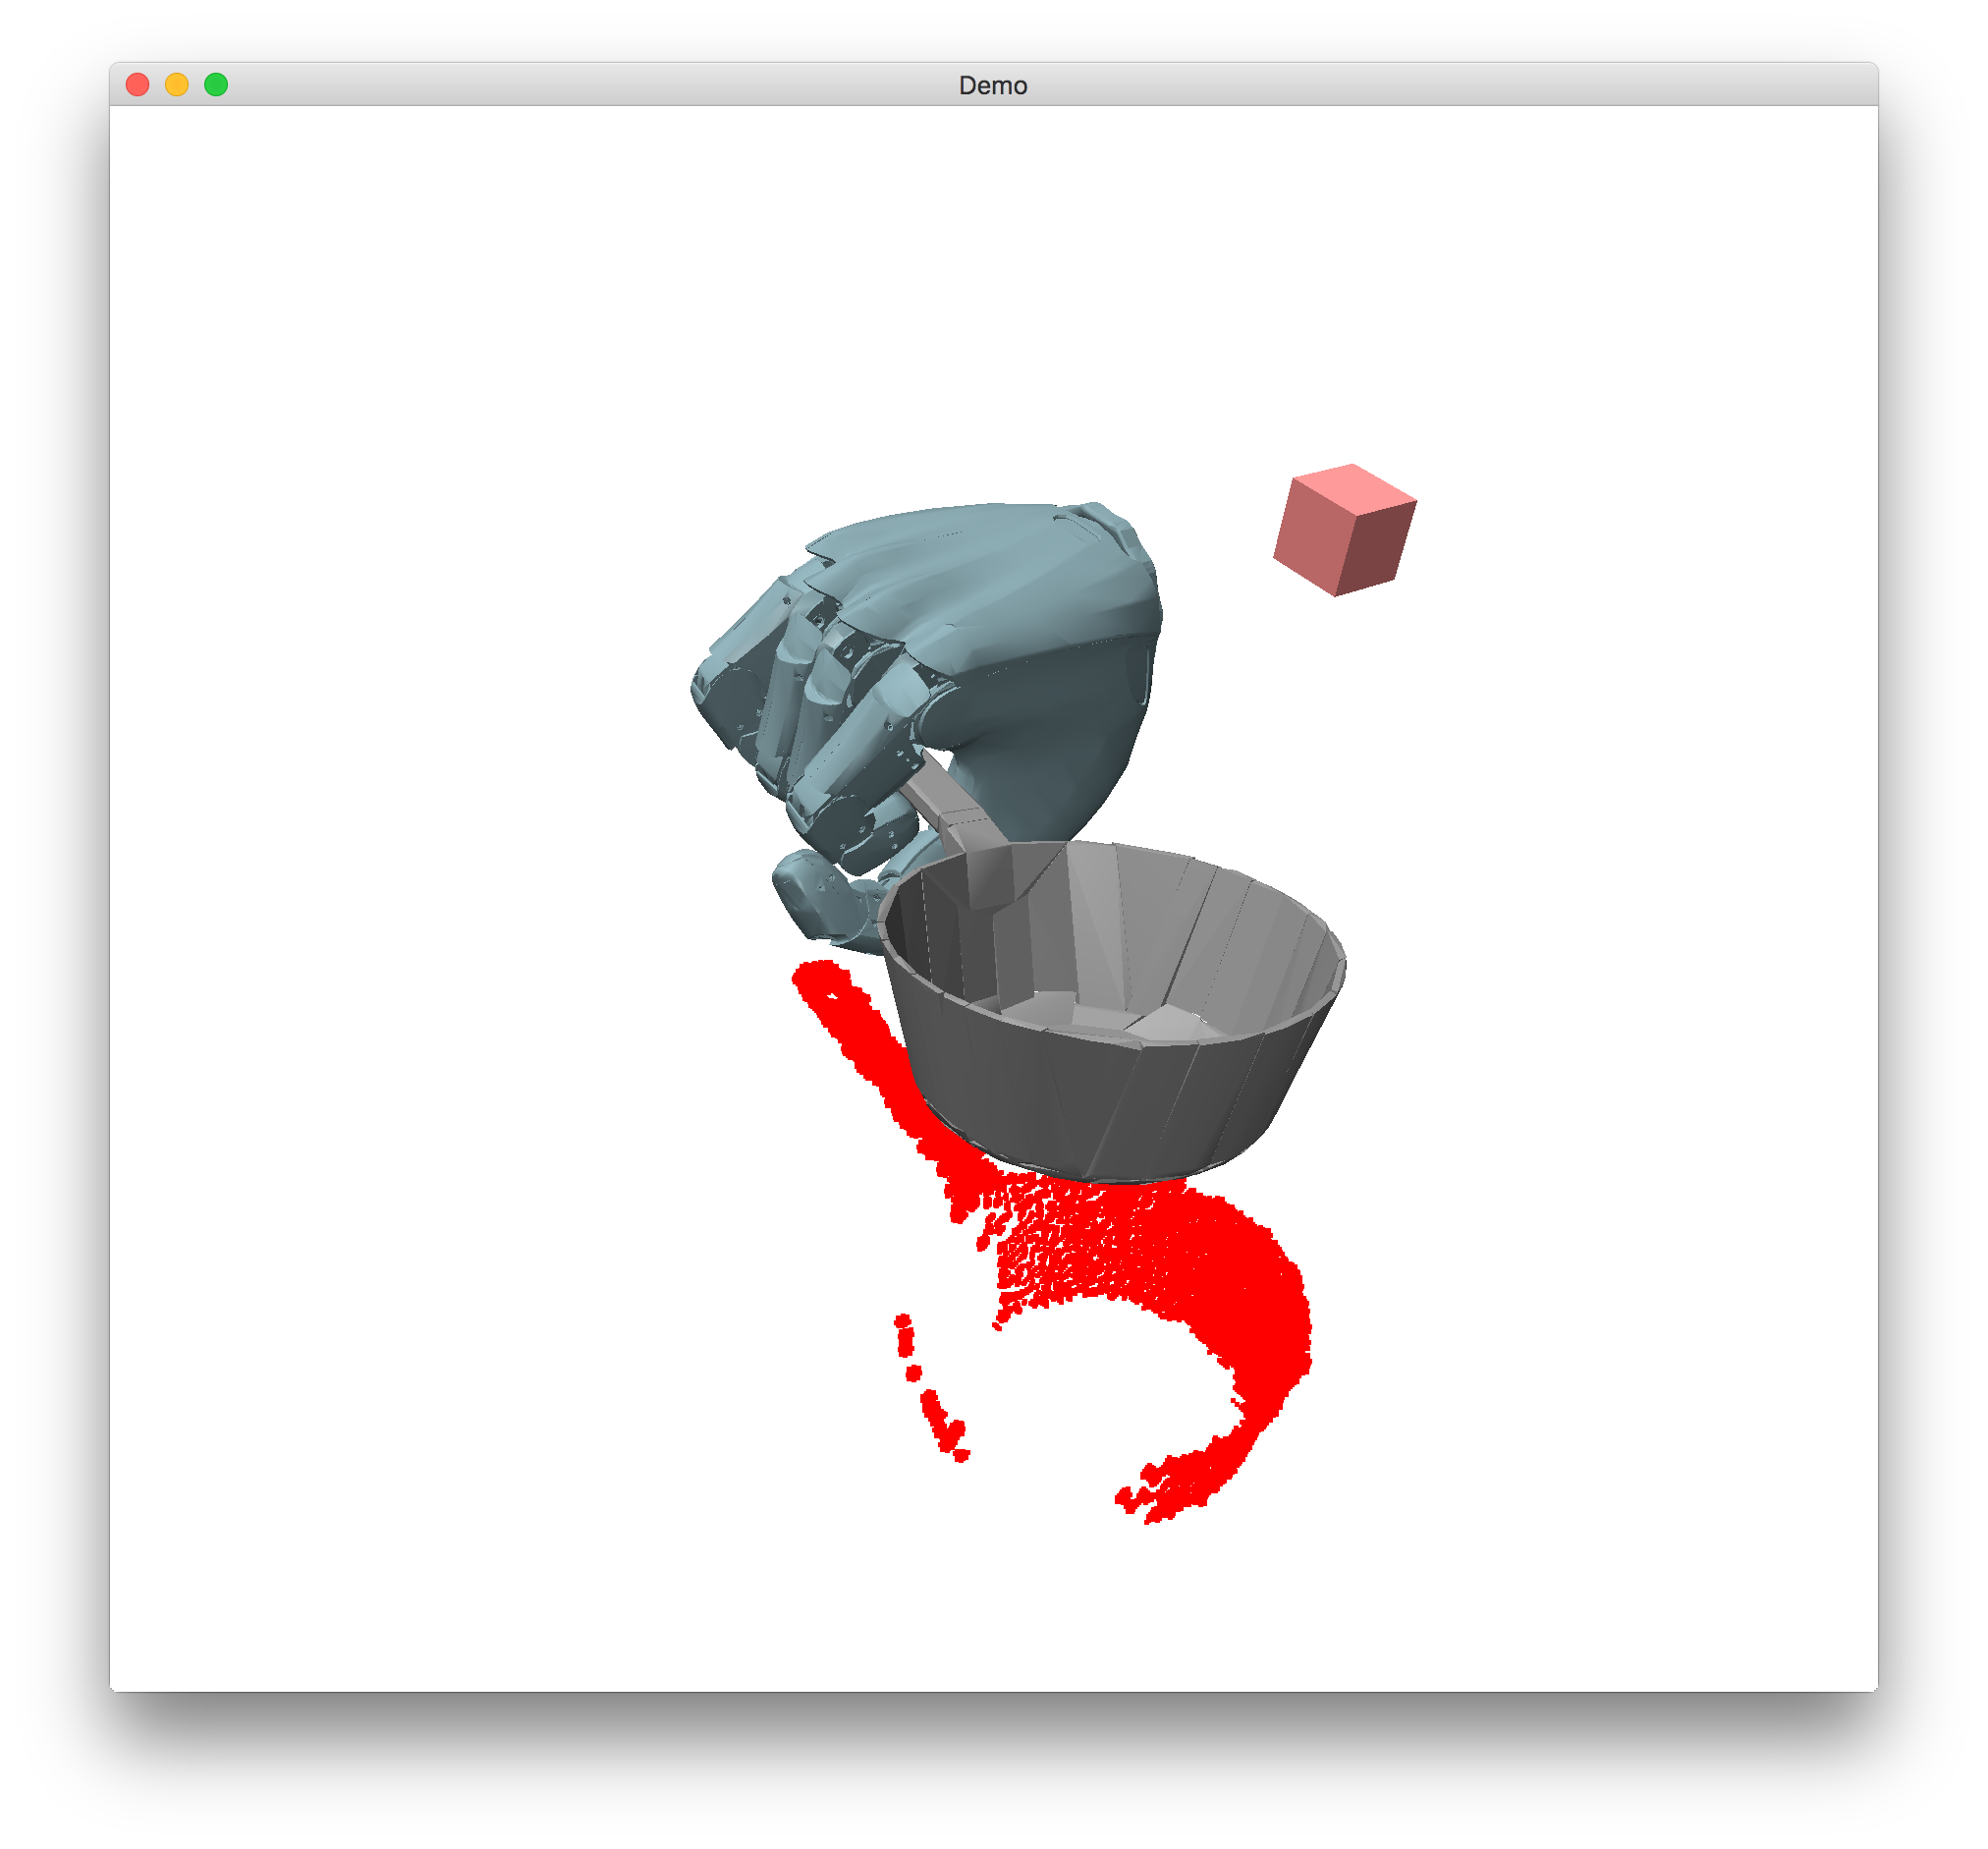
\includegraphics[width=0.24\textwidth]{images/Pan4_HFLW}
%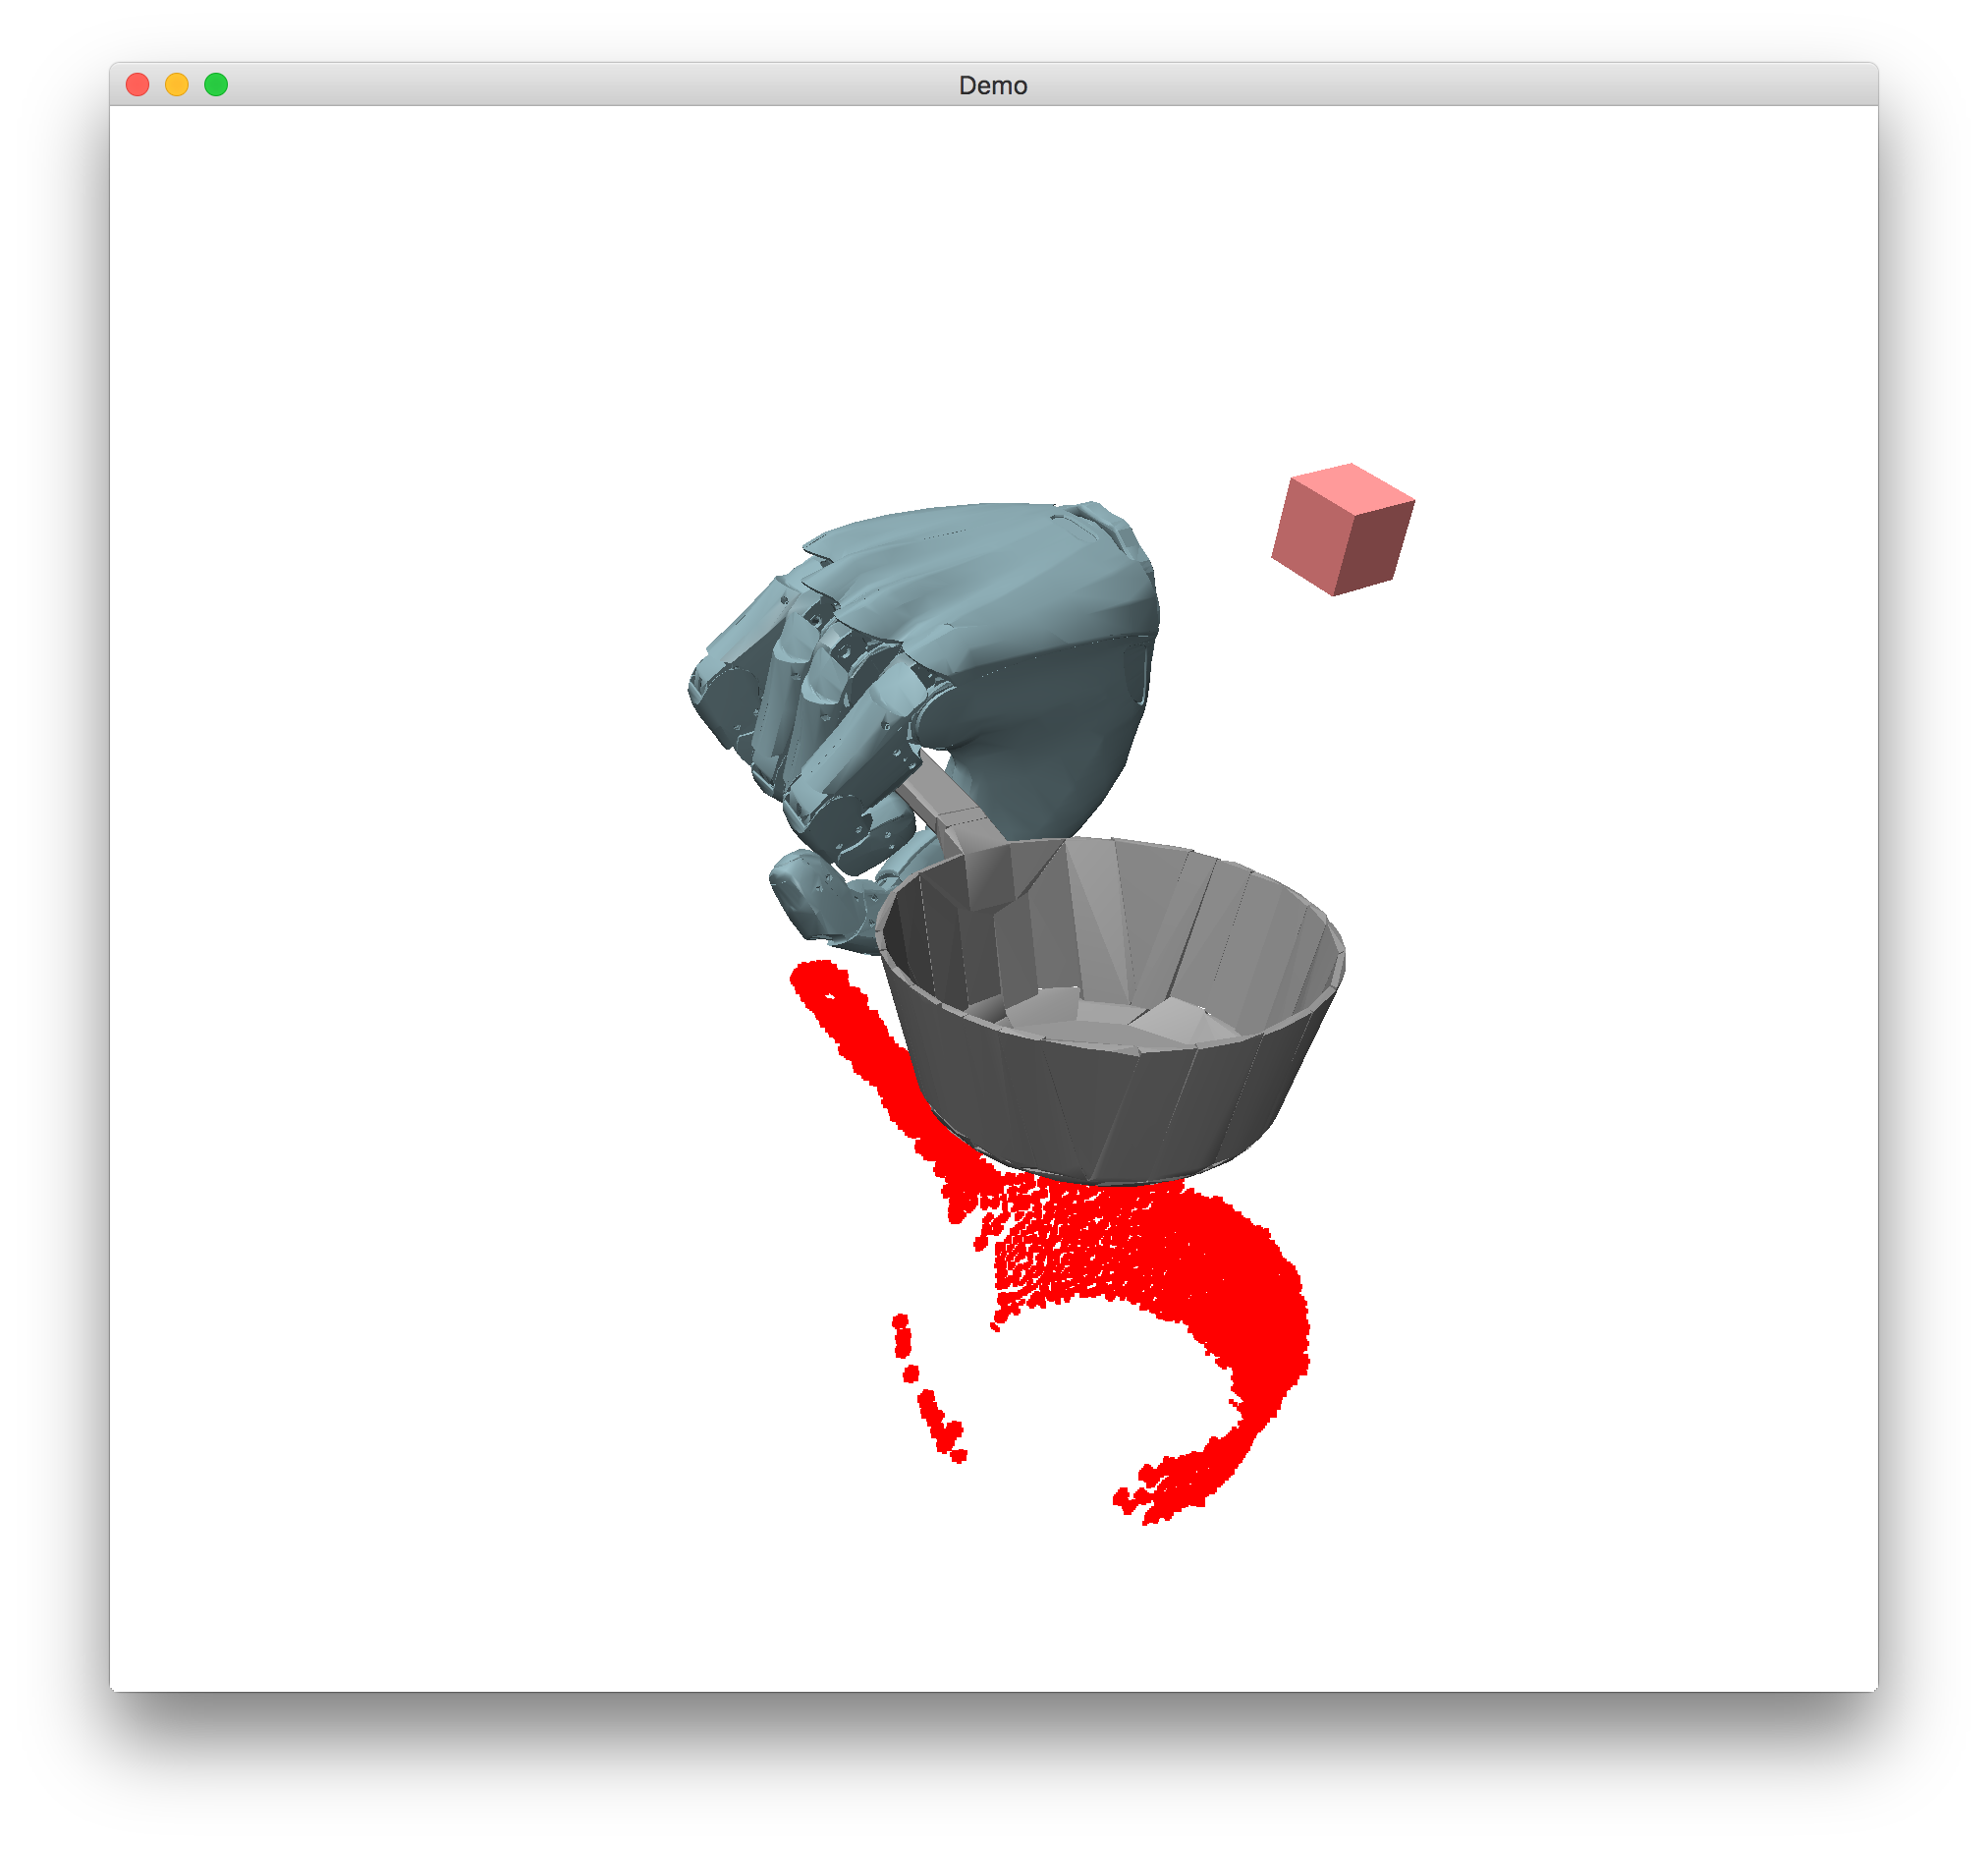
\includegraphics[width=0.24\textwidth]{images/Pan4_LFLW}
%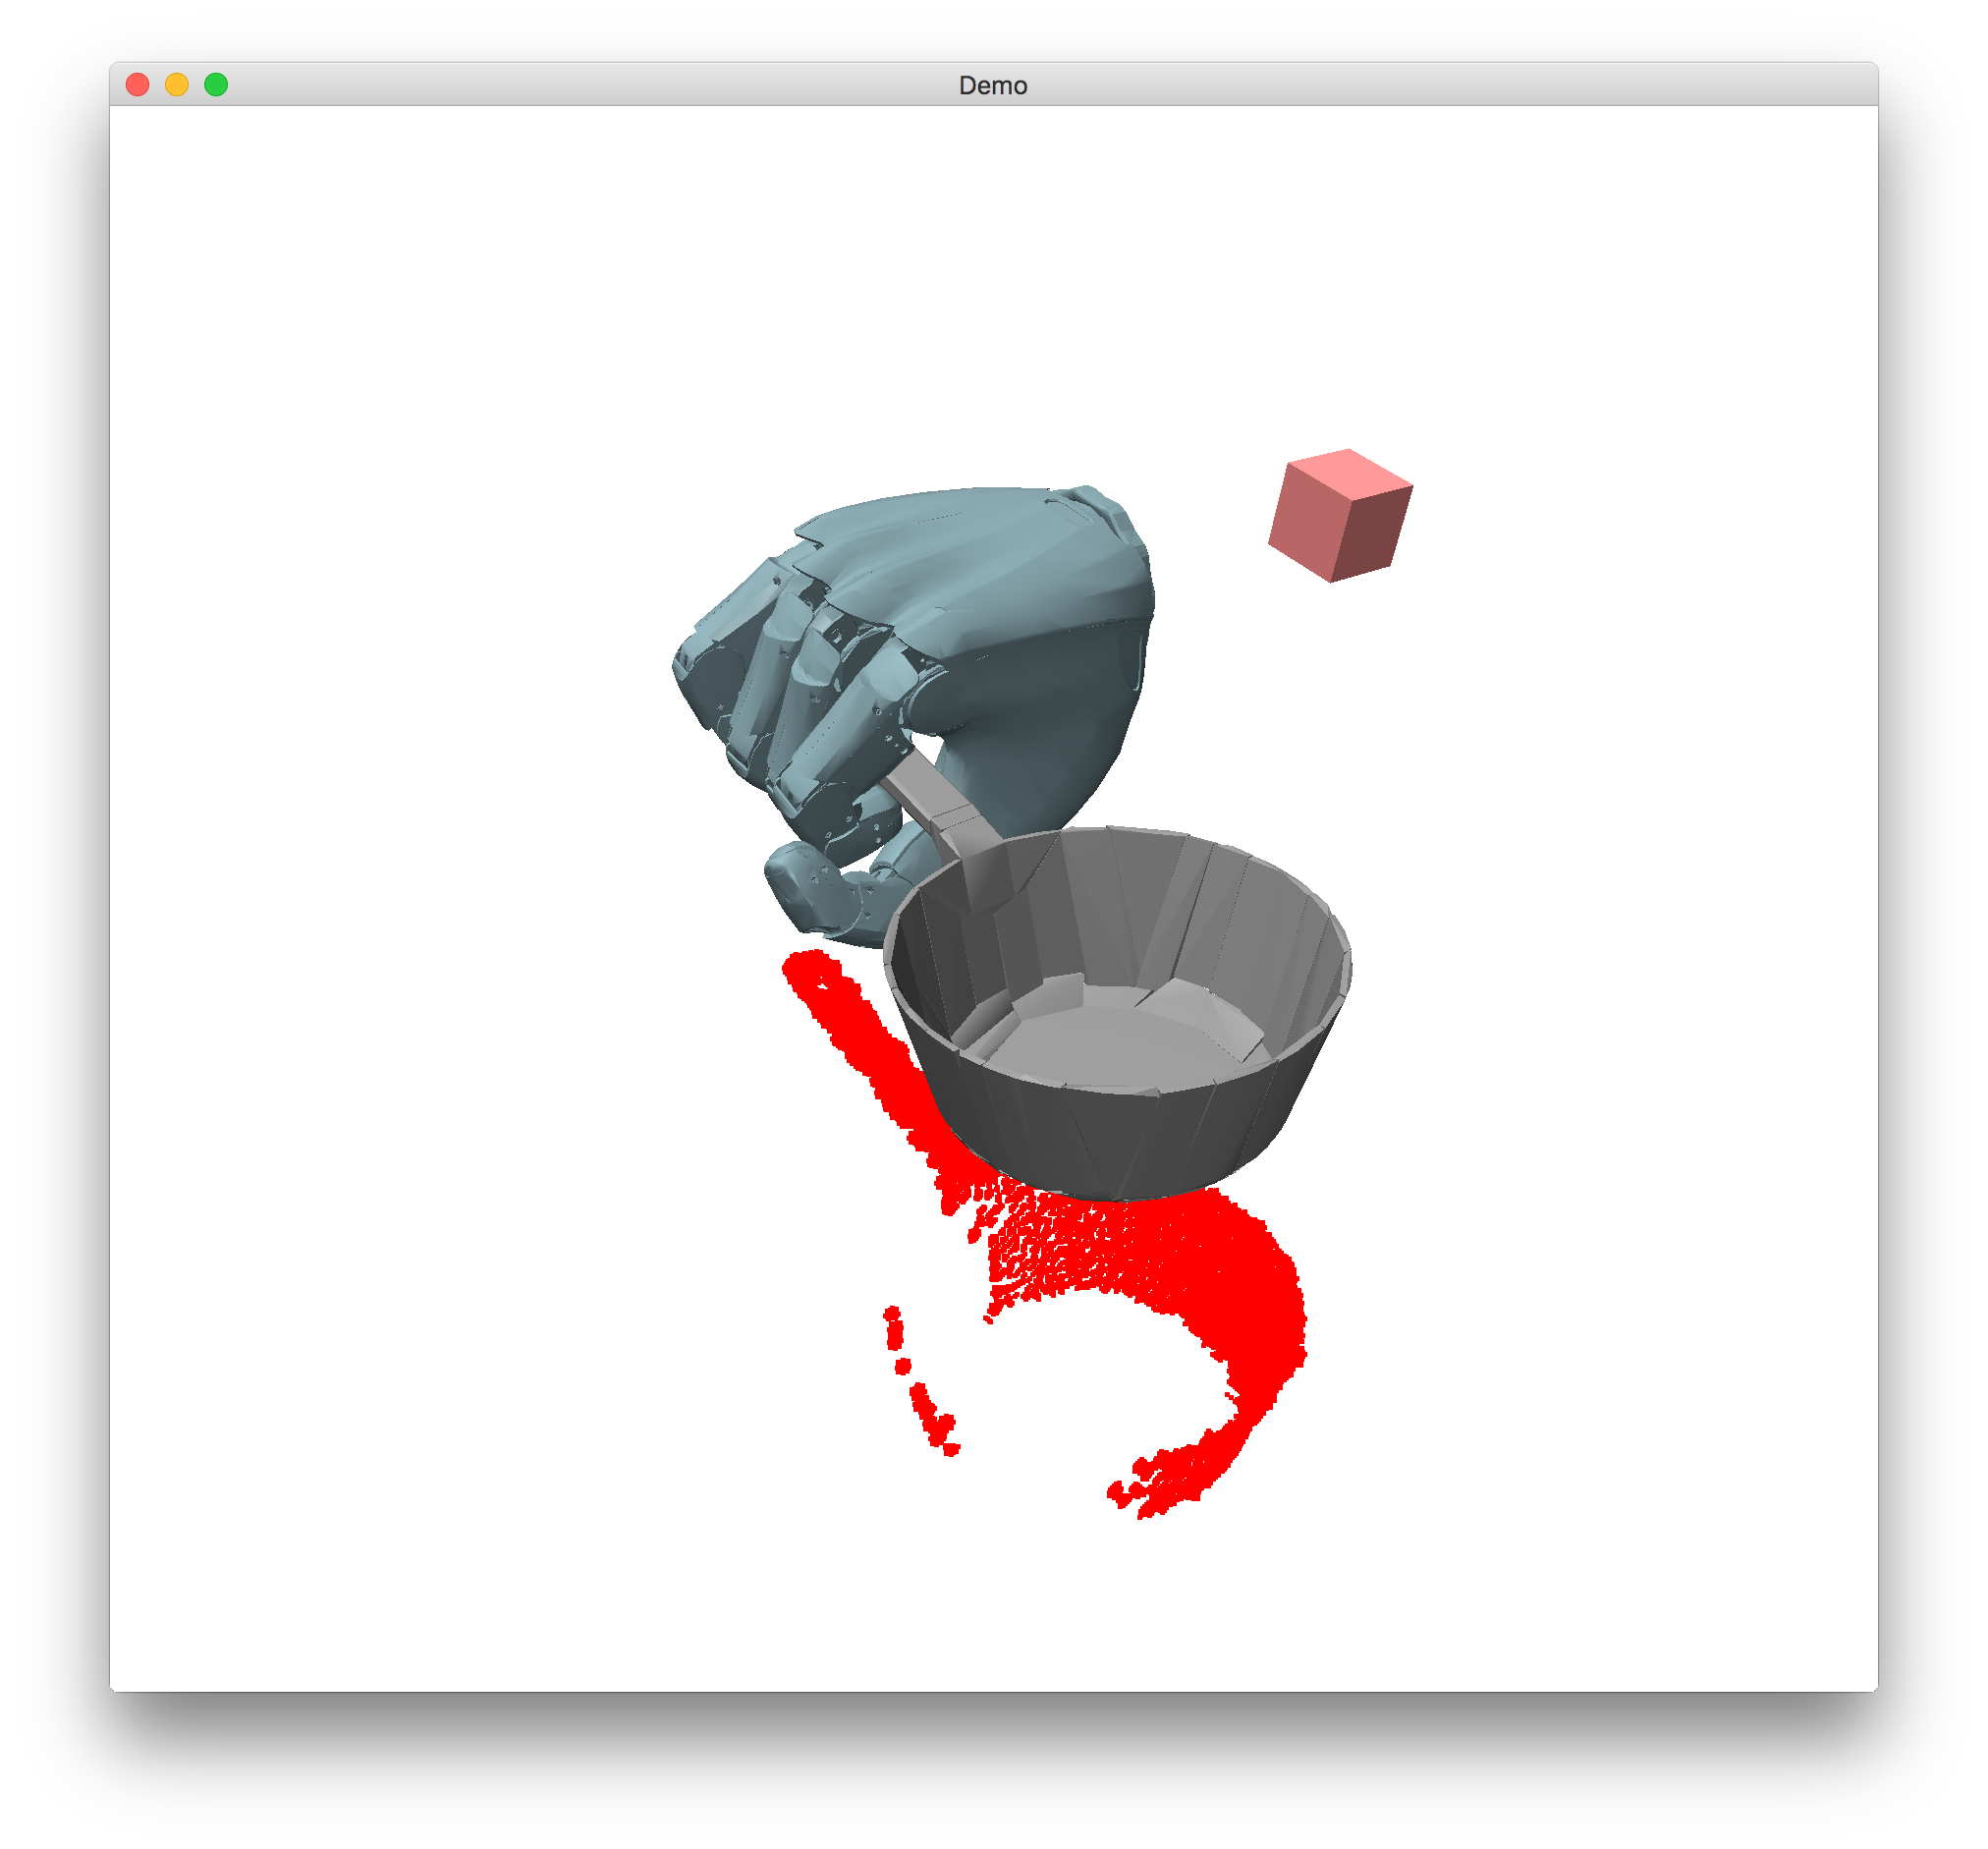
\includegraphics[width=0.24\textwidth]{images/Pan4_HFHW}
%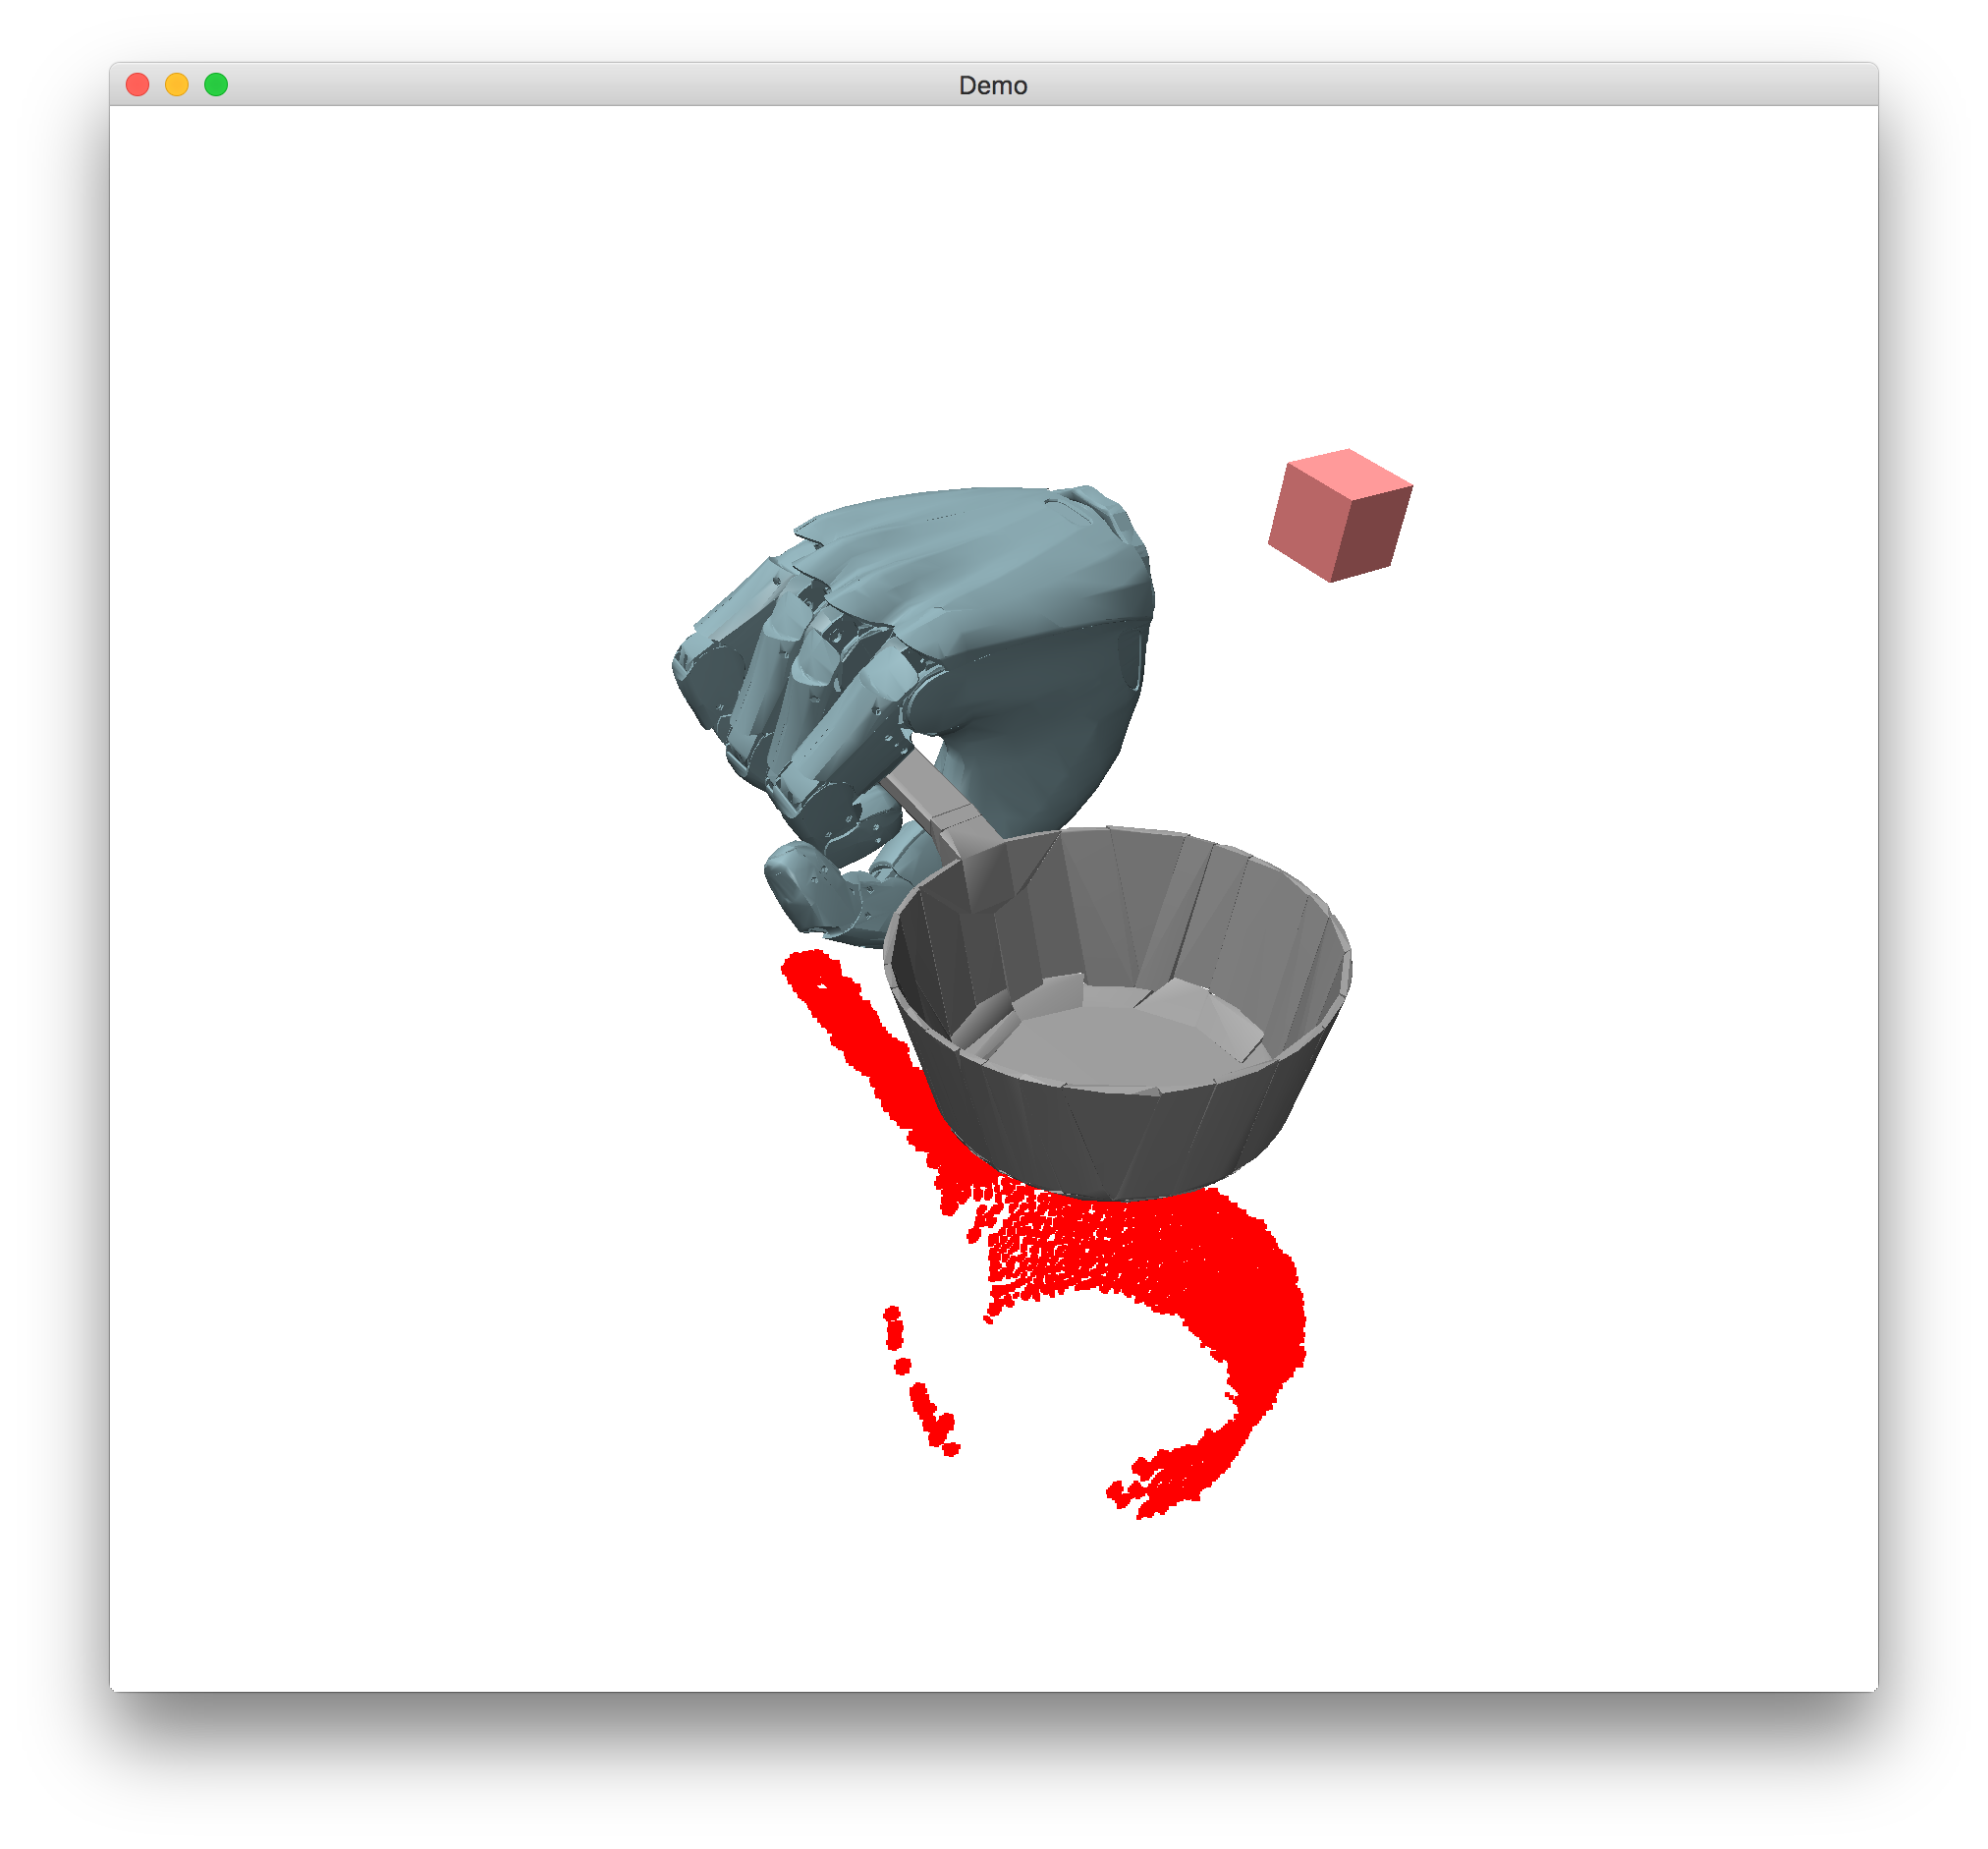
\includegraphics[width=0.24\textwidth]{images/Pan4_LFHW}
\caption{Creating a data set for robust evaluation. (Top row) The same pinch grasp, executed on the same object, with varying friction and mass parameters. (Bottom row) A more robust power grasp, executed on the same object, with the same variation in friction and mass. \label{fig:evaluative-training}}
\end{figure}

Using this method, we generated a data set (DS1) of 1.12 million simulated grasps using GM1 as the generative model and a data set of 1.136 million additional grasps (DS2) using GM2. Each grasp can be replayed in Mujoco and the set can be decomposed for train and test purposes as required. We give details of the statistics in Table including the way that we break down the data-set into training, validation and test subsets. The ratio of successful grasps in the dataset is less than 50\% for GM1, and is more than 50\% for GM2. In order to have a balanced training set, the number of successful and unsuccessful grasps have been equalised by under-sampling the failure cases in GM1 and over-sampling the failure cases for GM1. No balancing was performed for GM1/2 validation and test sets.
\begin{table*}[t]
\centering
\caption{Statistics of the simulated data sets.}
\label{tab:data}
\begin{tabular}{|l|l|l|l|l|l|l|l|l|l|l|} \hline
Data set & Generative &  Subset & \# Scenes & Top-grasp & Top-grasp & Top grasp & Total & Total  & Total  & Total \\ 
              & Model         &              &                   &  \# succs  & \# fails       & \% succs  & grasps   & \# succs      & \# fails  & \% succs  \\ \hline
 DS1-Tr & GM1 & Train & 17714 & 10100 & 7614 & 57.0\% & 959,882 & 479,941 & 479,941 & 50.0\% \\ \hline
 DS1-V  & GM1 & Validate & 1042 & 613 & 429 & 58.8\% & 61,393 & 29,557 & 31,836 & 48.1\% \\ \hline
 DS1-Te & GM1& Test & 1539 & 1070 & 469 & 69.5\% & 99,521 & 48,084 & 51,437 & 48.3\% \\ \hline
 DS2-Tr  & GM2 & Train & 5377 & 3771 & 1606 & 70.1\% & 943,481 & 533,282 & 410,199 & 56.5\% \\ \hline
 DS2-V   & GM2 & Validate & 544 & 378 & 166 & 69.4\% & 68,586 & 39,559 & 29,027 & 57.7\% \\ \hline
 DS2-Te  & GM2 & Test & 988 & 781 & 207 & 79.0\% & 124,137 & 73,836 & 50,301 & 59.5\% \\ \hline
\end{tabular}
\end{table*}

\section{The Generative Evaluative Architecture} \label{section:evaluative}
%In this section we describe how the evaluative models are trained and how we perform gradient descent and stochastic simulated annealing to attempt to improve grasps using the evaluative model.
\noindent
The grasping system proposed, shown in Figure \ref{fig:systemArchitecture}, consists of a learned generative model and an evaluative model. The generative model is a method that generates a number of candidate grasps given a point cloud, as explained in the previous section. An evaluative model is paired with a generative model in order to estimate a probability of success for each candidate grasp. All evaluative models process the visual data and hand trajectory parameters in separate pathways, and combine them to feed into a third processing block to produce the final success probability. In addition, we present techniques for grasp optimisation using the EM as the objective function, using both Gradient Ascent (GA) and Simulated Annealing (SA). Finally, we train each \textcolor{red}{evaluative model with data sets of simulated grasps generated using the generative models GM1 and GM2.} Table \ref{table:GEBreakdown} shows a the full list of 17 variants we test.

In this section, the three proposed evaluative model (EM) architectures are explained. The grasp generator models, GM1 and GM2, given in the previous section, require very little training data to train, here being trained from 10 example grasps. %GM1 can generate 500 candidate grasps, ranked according to their estimated likelihoods, within 10 seconds on a 2x Intel Xeon E5-2650 v2 Eight Core 2.6GHz. GM2 takes a 50 seconds to create 250 grasps in the same setting. 
These generative models do not, however, estimate a probability of success for the generated grasps. An evaluative model, which is a Deep Neural Network (DNN), is used specifically for this purpose. DNNs have shown good performance in learning to evaluate grasps using grippers \cite{levine16,lenz2015deep}. They have also been applied to generating pre-grasps, so as to perform power grasps with dexterous hands \cite{varley2015generating,lu2017planning}.

%The generative approach ignores the global information about the object, such as overall shape and the object category. The success of an executed grasp, however, depends on many contextual factors such as full object shape, mass, mass distribution and surface friction. An evaluative network can indirectly learn to predict grasp success from image data. 
%The data provided to the evaluative network is collected from randomly generated scenes, therefore each scene has a different random combination of the parameters. The primary purpose of the network is to learn robust grasps across different conditions, and this is a complex task. The first challenge is that the kinematic model of the hand is unknown to the evaluative network. It only has access to the parameters that \textit{configure} the hand: the wrist and joint positions. Second, the system is weakly supervised with the grasp result (success or failure), and no further labels are provided.

We tested three evaluative models. The first is based on the VGG-16 network \cite{Simonyan14c}, named Evaluative Model 1 (EM1), and shown in Figure \ref{fig:networkArchitecture2} (a). A version based on the ResNet-50 network, termed EM2, is shown in Figure \ref{fig:networkArchitecture2} (b). Finally, EM3 (Figure \ref{fig:networkArchitecture2} (c)) is also based on VGG-16. All EMs are initialised with ImageNet weights. Regardless of the type, an EM has the functional form $f(I_t, h_t)$, where $I_t$ is a colourised depth image of the object,\footnote{\textcolor{red}{Colourisation is a process by which additional channels are added to create a 3 channel representation. Here we add a channel encoding mean curvature and one encoding Gaussian curvature at that point in the depth image.}} and $h_t$ contains a series of wrist poses and joint configurations for the hand, converted to the camera's frame of reference.The network's output layer calculates a probability of success for the image-grasp pair $I_t$, $h_t$. The model processes the grasp parameters and \textcolor{red}{colourised depth} information in separate channels, and combines them to feed into a feedforward pipeline that produces the output.
\begin{table}[b]
\footnotesize
\centering
\begin{tabular}{|l|l|l|l|l|l|l|}
\hline
Variant & GM/  & EM & Opt'  & Training Set \\ 
 & Testset & & Meth' & \\ \hline
V1 & GM1    & - & - & 10 grasps  \\ \hline
V2 & GM2    & - & - & 10 grasps  \\ \hline
V3 & GM1/DS1-Te & EM1 & - & DS1-Tr \\ \hline
V4 & GM1/DS1-Te & EM2 & - & DS1-Tr \\ \hline
V5 & GM1/DS1-Te & EM3 & - & DS1-Tr  \\ \hline
V6 & GM1/DS1-Te & EM1 & - & DS1-Tr + DS2-Tr \\ \hline
V7 & GM1/DS1-Te & EM2 & - & DS1-Tr + DS2-Tr \\ \hline
V8 & GM1/DS1-Te & EM3 & - & DS1-Tr + DS2-Tr \\ \hline
V9 & GM2/DS2-Te & EM1 & - & DS1-Tr + DS2-Tr \\ \hline
V10 & GM2/DS2-Te & EM2 & - & DS1-Tr + DS2-Tr \\ \hline
V11 & GM2/DS2-Te & EM3 & - & DS1-Tr + DS2-Tr \\ \hline
V12 & GM1/DS1-Te & EM3 & GA1 & DS1-Tr + DS2-Tr \\ \hline
V13 & GM1/DS1-Te & EM3 & GA2 & DS1-Tr + DS2-Tr \\ \hline
V14 & GM1/DS1-Te & EM3 & GA3 & DS1-Tr + DS2-Tr \\ \hline
V15 & GM1/DS1-Te & EM3 & SA1 & DS1-Tr + DS2-Tr \\ \hline
V16 & GM1/DS1-Te & EM3 & SA2 & DS1-Tr + DS2-Tr \\ \hline
V17 & GM1/DS1-Te & EM3 & SA3 & DS1-Tr + DS2-Tr \\ \hline
\end{tabular}
\caption{The evaluated combinations of architecture, generative model/test set, training set, and optimisation method (Gradient Ascent (GA) or Stochastic Simulated Annealing (SA).}
\label{table:GEBreakdown}
\end{table}

%\begin{figure}[h]
%  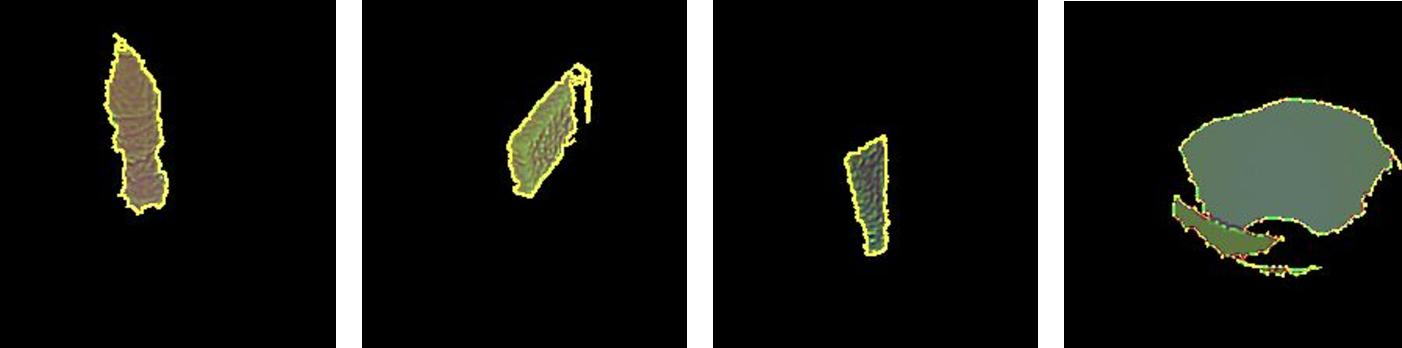
\includegraphics[width=0.9\linewidth]{images/colourDepth.pdf}
%  \caption[Colourised depth images.]{Colourised depth images. From left to right, the objects are: coke bottle, chocolate box, hand cream, and bowl.}
%\label{fig:colorisedDepth}
%\end{figure}
The single-channel depth image is colourised before it is passed as input to the evaluative network. For this, we first crop the middle $460 \times 460$ section of the $640 \times 480$ depth image, and down-sample it to $224 \times 224$. Two more channels of the same dimensions are added, corresponding to \textcolor{red}{the mean curvature and the Gaussian curvature}. %Figure~\ref{fig:colorisedDepth} contains four examples of colourised depth images. 
This procedure provides meaningful depth features to the network, and makes the input compatible with VGG-16 and ResNet-50, which require input images of size $224 \times 224 \times 3$.

The grasp parameter data $h_t$ consists of 10 trajectory waypoints represented by $27 \times 10 = 270$ floating point numbers, and 10 extra numbers reserved for the grasp type.\footnote{\textcolor{red}{Hand trajectory parameters are represented in the camera frame. Each waypoint has 27 float values: wrist position $(x,y,z)$ , wrist orientation (quaternion); finger joint angles (4 joints per finger, 5 fingers). Overall: 280 (10 + 10 * 27) floats per grasp.}} \textcolor{red}{Using trajectory information gives the network information it can use to predict unanticipated collisions with the object that will cause the grasp to fail.} Each of the 10 training grasps is treated as a different class, and $h_t$ uses the 1-of-N encoding system. The grasp parameters are converted to the coordinate system of the camera which was used to obtain the corresponding depth image. In EM1 and EM2, the parameters are processed with a fully-connected (FC-1024) layer and \textit{element-wise added} to the \textcolor{red}{learned} visual \textcolor{red}{representations}, while EM3 uses a convolutional approach. All networks join the \textcolor{red}{learned} visual features and grasp parameters in higher layers.

All FC layers have RELU activation functions, except for the output, which uses 2-way softmax in all EM variants. The output layer has two nodes, corresponding to the grasp success and failure probabilities. Cross-entropy loss is used. % to train the neural network, as given in \eq\ref{equation:crossentropy}.

All evaluative models in Table \ref{table:GEBreakdown} were trained and tested on simulated data. EM2 and EM3 were tested on the real robot setup. Variants V3-V5 were trained using DS1-Tr. Variants V6-V17 were trained using the combined data set from DS1-Tr and DS2-Tr \footnote{10\% of DS1-Tr failure cases were sampled from the grasps that collide with the table, and we preserved the colliding grasps in DS1-V. This was to ensure EMs do not propose such grasps. Training with DS2 did not involve colliding grasps since overall grasp quality of GM2 is better.}. The Gradient Descent(GD) optimiser was employed with starting learning rate of 0.01, a dropout rate of 0.5, and early stopping. We halve the learning rate every 5 epochs during training.


%\begin{equation}
%H_{y'}(y) := - \sum_{i} ({y_i' \log(y_i) + (1-y_i') \log (1-y_i)})
%\label{equation:crossentropy}
%\end{equation}
%where $y_i'$ is the class label of the grasp, which is either 1 (success) or 0 (failure), and $y_i = f(I_i, h_i)$ is is the predicted label of the grasp pair ($I_i$, $h_i)$.
The models are introduced below. Only their unique properties are highlighted.

\begin{figure*}[t!]
\centering
% \begin{center}
\subfloat[Evaluative Model 1]{%
  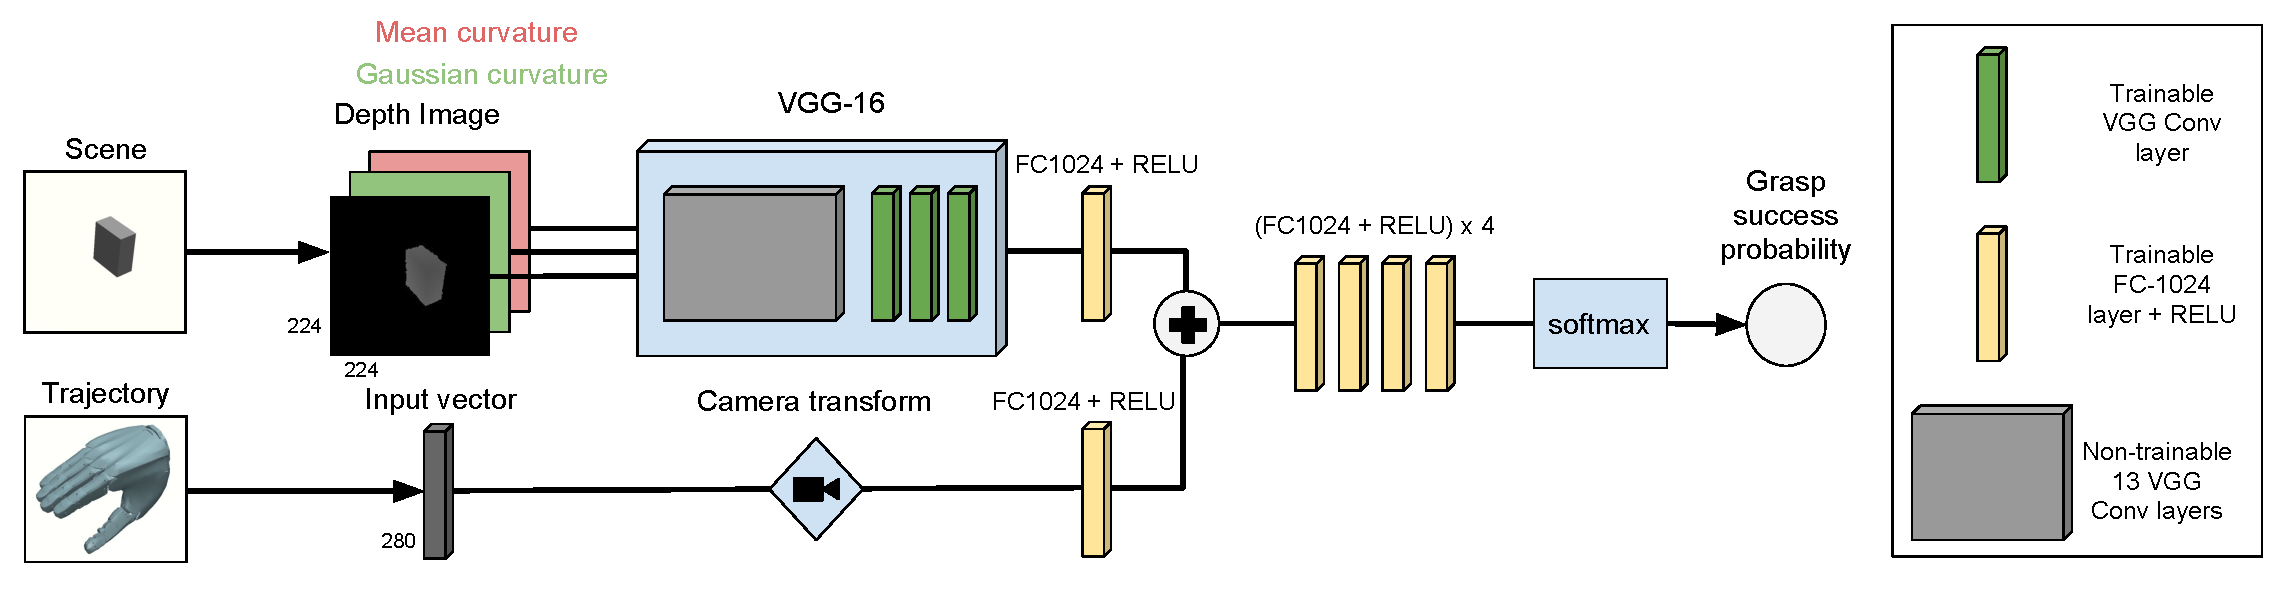
\includegraphics[width=0.91\textwidth]{images/networkArchitecture.pdf}
}
% \end{center}

% \begin{center}
\subfloat[Evaluative Model 2]{%
    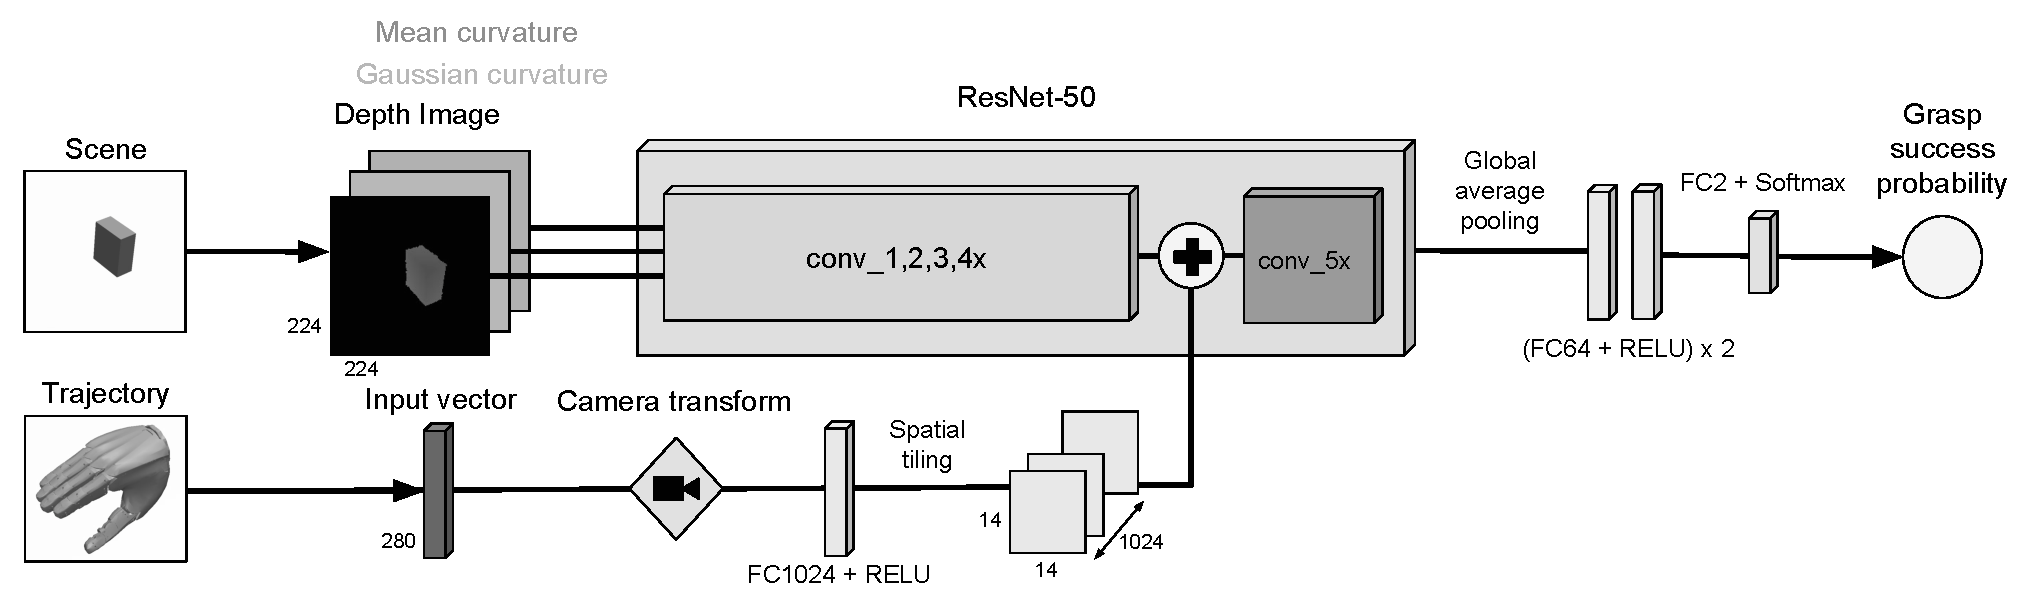
\includegraphics[width=0.91\textwidth]{images/ResNet.pdf}
}
% \end{center}

% \begin{center}
\subfloat[Evaluative Model 3]{%
    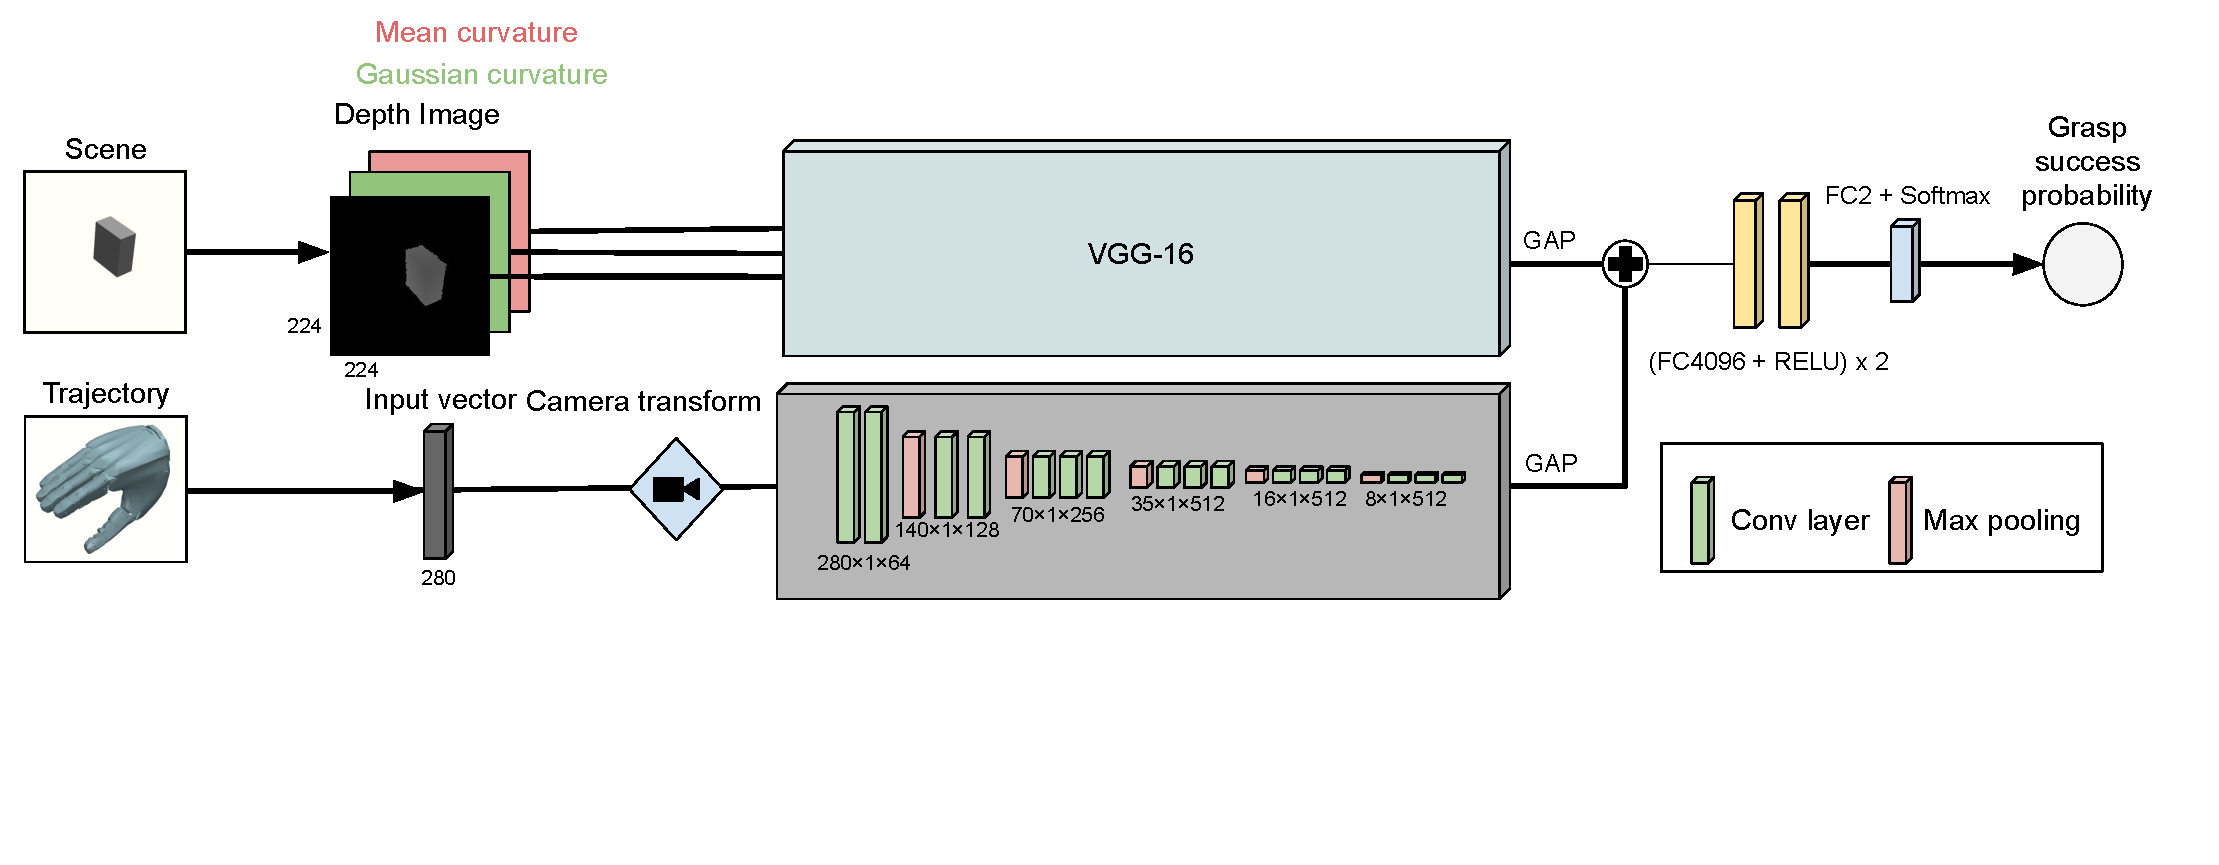
\includegraphics[width=0.91\textwidth]{images/Chaonet_newpic.pdf}
}
% \end{center}
\caption{The three evaluative network architectures. (a) EM1, a VGG-16 based model, where the first 13 layers of VGG-16 are frozen. (b) EM2, a ResNet-50-based network. The first four blocks are used for feature extraction and the rest to learn joint features. (c) EM3, also based on VGG-16.}
\label{fig:networkArchitecture2}
\end{figure*}

\subsection{Evaluative Models}

\noindent {\bf Evaluative Model 1 (EM1).}
\noindent
Figure~\ref{fig:networkArchitecture2} (a) shows the architecture of the first evaluative network. The colourised depth image is processed with the VGG-16 network \cite{Simonyan14c}. The first 13 layers are frozen to reduce overfitting. Grasp parameters and image features each pass through two FC-1024 layers to obtain two feature vectors of length 1024. The features are combined using element-wise addition and fed into 4 FC-1024 layers. Concatenation and addition can be considered as interchangeable in this context \cite{dumoulin2018feature-wise}. The final FC-1024 layers form associations between visual features and hand parameters, and contain most of the trainable parameters in the network.

\noindent {\bf Evaluative Model 2 (EM2).}
\noindent
% \begin{figure}[!ht]
%   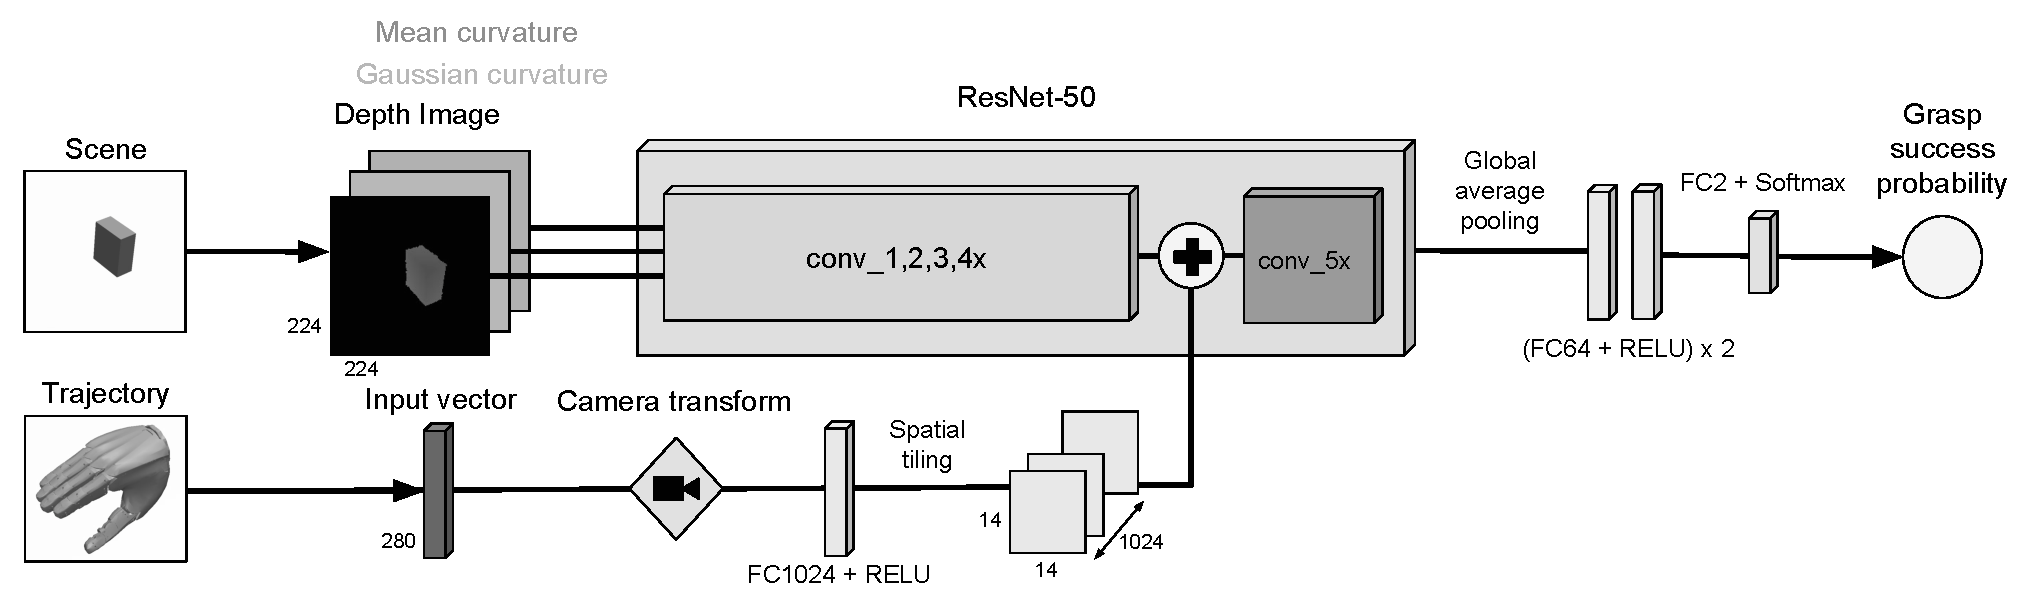
\includegraphics[width=\textwidth]{images/ResNet.pdf}
%   \caption[The ResNet-based evaluative deep neural network architecture.]{The ResNet-based evaluative deep neural network architecture (EM2). Spatial tiling is used to repeat the grasp parameters before they join the image processing pathway. This network requires fewer FC layers due to the earlier marriage of information channels.}
% \label{fig:ResNet}
% \end{figure}
EM2 (Figure~\ref{fig:networkArchitecture2} (b)) uses the ResNet-50 architecture \cite{HeZRS15}, broken down into two parts. The first 4 convolutional blocks are used to extract the visual features. The final block, with 9 randomly-initialised convolutional layers, combines these with the grasp parameters. Similar to EM1, element-wise addition joins the two channels. The grasp parameters, a vector of size $1024$, are repeated to form a block of size $14 \times 14 \times 1024$. The final block processes the merged information and has 2 FC-64 layers.

\noindent {\bf Evaluative Model 3 (EM3).}
\noindent
This model (Figure~\ref{fig:networkArchitecture2} (c)) also uses VGG-16, but all 16 layers are trainable. The hand trajectory parameters pass through a feature extraction network before being concatenated with the visual features. The combined part of the network contains two high-capacity FC-4096 layers, followed by a FC2+softmax layer. EM3, in contrast to EM1 and EM2, uses convolutional layers for processing input grasp trajectories. The trajectory sub-network is similar to VGG-16 in that it contains 5 blocks, comprising 13 convolutional layers. The convolutional filters have a width of 3. The sizes under the blocks are input dimensions. Global Average Pooling (GAP) is used to obtain 512 features from each side, which are concatenated and passed through two FC-4096 layers. 

\subsection{Grasp optimisation using the EM}
\noindent
So far we have considered only generative-evaluative architectures where the evaluative model (EM) merely ranks the grasp proposals. As proposed by Lu et al. \cite{lu2017planning} \textcolor{red}{the EM can be used to improve grasp proposals}. This boils down to searching the grasp space driven by the EM as the objective function. This may be by gradient ascent or simulated annealing. The methods V12-17 use V8 as the objective function, hence V8 should be treated as the baseline. We employed both gradient based optimisation and simulated annealing.

\subsubsection{Gradient based optimisation}
\noindent
Lu et al. \cite{lu2017planning} proposed gradient ascent (GA), modifying the grasp parameters input to the EM with respect to the output, predicted success probability. They initialised with a heuristically selected pre-grasp. \textcolor{red}{It is an interesting question whether we can apply their method to our evaluative models so as to further improve the performance. We therefore apply their technique initialised with the highest ranked grasp according to the EM.} We investigated three variants:
\begin{itemize}
\item GA1: Shifts the position of all of the waypoints in the grasp trajectory equally. The gradient is the average position gradient across all 10 waypoints.
\item GA2: Tunes the hand configuration by tuning the angle of each finger joint. Every finger joint at each waypoint is treated independently.
\item GA3: Performs GA1 and GA2 simultaneously.
\end{itemize}

\subsubsection{Simulated annealing based optimisation}
\noindent
Gradient based optimisation is sensitive to the quality of gradient estimates derived from the model. Simulated annealing (SA) based optimisation is more robust to such noise. Therefore, three optimisation routines were implemented using SA:
\begin{itemize}
\item SA1: Shifts the positions of the all waypoints in the grasp trajectory equally. Moves are drawn from a three-dimensional Gaussian with $\mu=0$ and $\sigma=0.001$. 
\item SA2: Scales the angles of the finger joints in the final grasp pose with a single scaling parameter drawn from a Gaussian with $\mu=1$ and $\sigma=0.001$. The initial finger joint angles remain fixed and joint angles of the intermediate waypoints are linearly interpolated. 
\item SA3: Performs SA1 and SA2 simultaneously.
\end{itemize}


\section{Simulation Analysis}
\label{section:simulationAnalysis}
This section presents a simulation analysis of the various architectures based on the two data sets. 
We assess each variant in two different ways. First, for any method with an evaluative model we  measure the prediction accuracy of the EM. We compare the actual outcomes in a test set with the EM's prediction as to whether it is more likely to succeed or fail (output set at a threshold of 0.5). This gives us a confusion matrix from which we can calculated sensitivity, specificity and F1 score. Second, since a robot can only execute one grasp, we can measure the proportion of successful top-ranked grasps for any method. In each analysis the test set effectively replaces the Generative Model as it contains, for any scene, a complete list of grasps. Thus TS1 contains grasps proposed by GM1 and TS2 contains grasps proposed by GM2. This allows us to simulate the effect of different generative models on performance. 

We performed both analyses and the results are given in Table~\ref{table:Results-sim}. When assessing pure GM architectures, we can only measure the top ranked grasp success, since the GMs give a grasp likelihood according to the generative model not a probability of success. 

The main findings are as follows. First, of the pure generative models GM2 outperforms GM1, with top ranked grasp successes of 79.05\% and 69.53\% respectively. Second, the GEA architectures all outperform both pure GM architectures, starting at 87.85\% of grasps succeeding (V3 based on proposals from GM1 and evaluation by EM3 trained on TS1). Third, the increase in training set size (adding GM2 to GM1) yields a further improvement. We can best measure this by considering the residual number of top grasps that fail as a percentage of the baseline (GM1). On this measure adding the additional data (variants V6-V9) improves performance (over variants V3-V5) by an average of 3\%. 

All the above results use GM1 as the generative model. We can measure the benefit of substituting this by GM2. This yields a further reduction in residual failures over GM1 under the same training conditions (training with DS1-Tr and DS2-Tr) of 3.5\%. 

In summary, simulation results provide evidence that: pure GM2 outperforms GM1; adding training data improves results; and using GM2 as the generative model in the generative-evaluative architecture improves results. 

%Recall that the generative-evaluative architecture (GEA) comprises both the generative model (GM) and the evaluative model (EM). 
%We can evaluate aspects of these separately. After training, the EM was used to predict grasp outcomes in the test set. This comprised 1,241 scenes with 76,213 grasps. Of these, 40,243 succeeded and 35,970 failed. Our analysis is given in Table~\ref{fig:predictions}. The sensitivity is 0.84 and the specificity 0.71. The F1-score is 0.802.
%\begin{table}[b]
%\centering
%\caption{Confusion matrix for prediction on simulated data.}
%\label{fig:predictions}
%\begin{tabular}{|c|c|c|c|c|c|}
%\hline
% & & \multicolumn{4}{c|}{Prediction} \\ \cline{3-6}
%      & & \multicolumn{2}{c|}{\#} & \multicolumn{2}{c|}{\%} \\ \cline{3-6}
%  &  & Succ         & Fail         & Succ         & Fail         \\ \hline
%\multirow{ 2}{*}{Ground Truth} \newline & Succ & 33890      & 6353       & 84\%     & 16\%       \\ \cline{2-6}
% &Fail & 10339      &  25631    & 29\%     &  71\%   \\ \hline
%\end{tabular}
%\end{table}
% In this context, precision is the fraction of correctly labeled grasps among those predicted to be of a certain class (success or failure). Recall stands for the fraction of relevant grasps that have been identified correctly among all grasps that belong to that class. The results show a high recall rate for successful grasps, and there are relatively more false positives than false negatives. This necessitates pairing our evaluative neural network with a generative model rather than a random grasp generator, which would likely result in very low quality grasps and consequently, more false positives. 

%To test our generative-evaluative learning architecture we compared the grasp it proposes to the grasp proposed by the generative learner alone. Since \citet{kopicki2015ijrr} showed a 77.7\% success rate with the original generative algorithm we generated a new test set that contained both more challenging objects and placed them in challenging poses. The difficulty single-view grasping with a depth camera depends greatly on the pose of the object relative to the camera. The set comprised 40 test objects (Figure~\ref{fig:real-objects}) and another six training objects. The training objects were used by the human to demonstrate ten example grasps (Figure~\ref{fig:generative-training}). The 40 test objects were used to generate 49 object-pose pairs. From the 40 objects, 35 belonged to object classes in the simulation dataset, while the remaining five do not. 

\begin{figure}[t]
  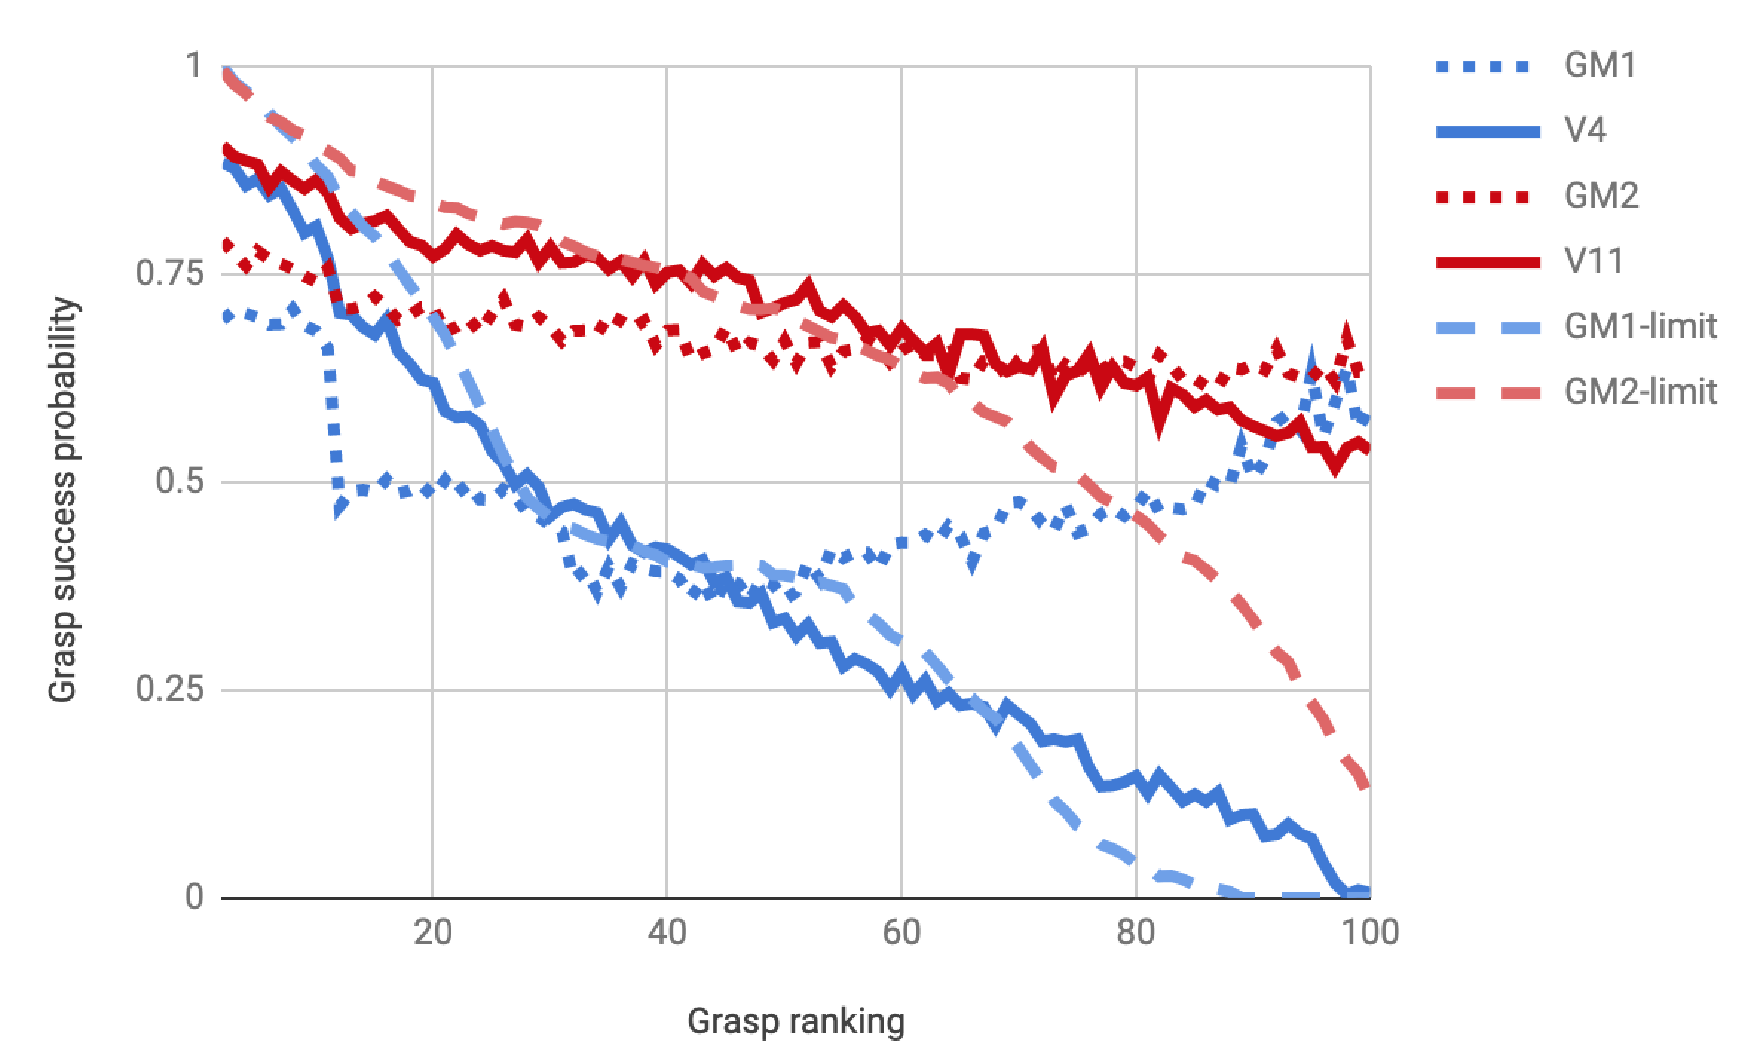
\includegraphics[width=\linewidth]{images/successvsranking.pdf}
  \caption{Grasp success probability (in simulation) vs. grasp ranking. GEA2 and GEA3 use GM1 and GM2 test data, respectively.}
  \label{fig:successvsranking}
\end{figure}

%We compared the EM and GM rankings (Figure~\ref{fig:successvsranking}). The x-axis shows the ranking. The y-axis shows the average actual success rate over all scenes (1,241 test, 7,311 training). When ranked by the EM, the grasp success probability falls nearly monotonically, as is desirable. On the other hand, the likelihood-based ranking of GM results in many good grasps being low-ranked. We also wish to know whether the grasps recommended by the EM and the GM have different grasp success rates. The success rates of the top-ranked grasps are 71.59\% (GM) and  84.2\% (EM).
So far we have considered only Generative-Evaluative architectures where the Evaluative Model merely ranks the grasp proposals. We also investigated using the EM to improve these grasps proposals. This essentially boils down to searching the grasp space driven by the EM as the objective function. This can be done either by gradient descent or using simulated annealing. The methods V12-17 use V11 as the objective function, hence V11 should be treated as the baseline. 

Lu et al. \cite{lu2017planning} proposed gradient ascent on the input grasp parameters to the EM with respect to the predicted success probability. They initialised with a heuristic grasp. We initialise with the best grasp proposed by the GEA. We experimented with three variants of the gradient ascent based tuning:
\begin{itemize}
\item GD1: Moves the entire trajectory at once in the world coordinate space, as directed by the average gradient on the trajectory's all 10 waypoints.
\item GD2: Tunes each finger joint individually. Each waypoint is treated independently.
\item GD3: Performs GD1 and GD2 simulatenously.
\end{itemize}

We ran the optimisation for 50 iterations, using a learning rate of 0.001 for position inputs and 0.01 for finger joints (We used different learning rates since the parameters are in different scales, GD1 in meters and GD2 in radians). Although predicted success rate rises, the success rate in simulation declines in all trials. We observed that the position changes have a more significant negative impact on the grasp success rate, when compared to finger joint movements. The results suggest that optimising dexterous grasps by the EM is non-trivial, perhaps because of the high-dimensionality of the grasp space. We speculate that initialising with a random grasp would be even worse.

Additionally, we implemented three variants of simulated annealing based optimisation:
\begin{itemize}
\item SA1: Moves the entire trajectory at once in the world coordinate space, using a three-dimensional Gaussian noise vector, with $\mu=0$ and $\sigma=0.001$. 
\item SA2: Perturbs the finger joints along the entire trajectory. The pose of all joints in a finger with respect to a reference pose (fully open hand) is modified, which results in an "opening/closing the finger" effect. We observed that this is a more natural movement rather than modifying a finger's joints independently. The opening/closing ratio for each finger is determined by a noise vector that is drawn from a Gaussian distribution with $\mu=0$ and $\sigma=0.01$. 
\item SA3: Performs SA1 and SA2 simulatenously.
\end{itemize}

The simulated annealing procedure contains up to 5 iterations, with 20 random perturbations in each. We start with a temperature of 0.2 and decrease it exponentially to 0.005 by halving it after every batch. If the current solution does not improve after three iterations, the optimisation stops. We do not accept any perturbations that will result in a collision with the table. Similarly with gradient ascent, the performance of the optimised grasps are worse than the baseline (V11). The effect of moving the trajectory is more significant when compared to the finger joints. TODO: Interpret the results.

\begin{table*}[t]
\centering
\begin{tabular}{|l|l|l|l|l|l|l|l|l|l|l|}
\hline
Variant \# & \multicolumn{2}{|c|}{Selected grasp} &  Succ \% & Residual Fails & Test set / GM& \multicolumn{5}{|c|}{Prediction Performance} \\ \hline
 & Succs & Fails &  & as \% of V1 fails &  & TP & FP & TN & FN & Accuracy \\ \hline
V1 & 1070   & 469 & 69.53\% & 100\% & GM1 & - & - & - & - & - \\ \hline
V2 &  781   & 207 & 79.05\% & 68.7\% & GM2 & - & - & - & - & - \\ \hline
V3 & 1352 & 187 & 87.85\% & 39.9\% & GM1 & 37840 &	12226 & 39211 & 10244 & 77.42\% \\ \hline
V4 &  1361 & 178 & 88.43\% & 38.0\% & GM1 & 40234 &	14475 & 36962 & 7850 & 77.57\% \\ \hline

V5 & 1361 & 178 & 88.43\% & 38.0\%& GM1 & 39603 & 14122 &37315 & 8481	& 77.29\% \\ \hline

V6 & 1375 & 164 & 89.34\% & 35.0\% & GM1 & 37584 &	11514 & 39923 &10500	& 77.88\% \\ \hline
V7 & 1363 & 176 & 88.56\% & 37.5\% & GM1 & 39332 &	12020 & 39417 & 8752 & 79.13\% \\ \hline
V8 & 1378 & 161 & 89.54\% & 34.3\% & GM1 & 37832 &	11361 & 40076	& 10252 & 78.28\% \\ \hline
V9 & 887 & 101 & 89.78\% & 33.5\% & GM2 & 61866 &	11454& 38847& 11970 & 81.13\% \\ \hline
V10 & 893 & 95 & 90.38\% & 31.6\% & GM2 & 64309 &	12517 & 37784 & 9527 & 82.24\% \\ \hline
V11 & 894 & 94 & 90.49\% & 31.2\% & GM2 & 61611 & 9792 & 40509 & 12225 & 82.26\% \\ \hline
V12 & 1319 & 220 & 85.71\% & 47.0\% & GM1 & - & - & - & - & - \\ \hline
V13 & 1375 & 164 & 89.34\% & 35.0\% & GM1 & - & - & - & - & - \\ \hline
V14 & 1366 & 173 & 88.76\% & 37.0\% & GM1 & - & - & - & - & - \\ \hline
V15 & 1153 & 386 & 74.92\% & 82.0\% & GM1 & - & - & - & - & - \\ \hline
V16 & 1377 & 162 & 89.47\% & 35.0\% & GM1 & - & - & - & - & - \\ \hline
V17 & 1163 & 376 & 75.57\% & 80.0\% & GM1 & - & - & - & - & - \\ \hline
\end{tabular}
\caption{Simulation results for all variants tested.}
\label{table:Results-sim}
\end{table*}
%A pure generative model architecture (GM) and the generative-evaluative architecture (GEA) were evaluated using a paired trials methodology. Each was presented with the same object-pose combinations. Each architecture generated a ranked list of grasps, and the highest ranked grasp was executed. The highest-ranked grasp based on the predicted success probability of the network is performed on each scene. A grasp was deemed successful if, when lifted for five seconds, the object then remained stable in the hand for a further five seconds before being automatically released. The success rate for GM was 57.1\% and for GEA it was 77.6\%. The successes and failures for each method were recorded and are summarised in Table~\ref{tab:robot-results}. A two-tailed McNemar test, for the difference between success rates for paired comparison data, was performed and the difference between the two algorithms has a $p$-value of 0.0442, and so is statistically significant. A selection of grasps where the two methods performed differently are shown in Figure~\ref{fig:successfail}.

% OLD TABLE
%\begin{table}
%\begin{center}
%\caption{Results of the real robot paired comparison trial.}
%\begin{tabular}{|c|c|c|c|}  \hline 
%          &                & \multicolumn{2}{ c |}{ GM} \\ \hline
%          &                & \# succs & \# fails  \\  \hline
 %GEA  & \# succs &  23 &  15  \\
 %         & \# fails    &  5   &   6   \\ \hline
%\end{tabular}
%\end{center}
%\label{tab:robot-results}
%\end{table}

%Training parameters for network. Training of example grasps for learning from demonstration. Creation of real test data set. Paired comparisons methodology with vanilla LFD algorithm (pose + object + camera view).
%
%The actual grasping tests have been performed on the real robot. 

\section{Real robot experiment}
\label{section:experiments}

\begin{figure}[t]
\begin{center}
  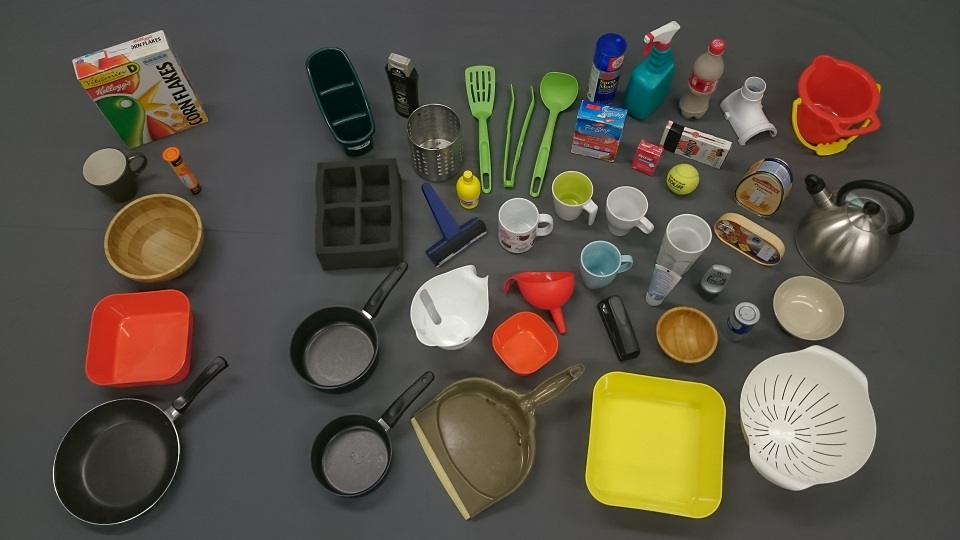
\includegraphics[width=0.7\linewidth]{images/objects.jpg}
  \end{center}
  \caption{The real objects. The training objects are on the left, testing objects are on the right.}
  \label{fig:real-objects}
\end{figure}

\begin{table}[b]
\small
\begin{center}
\caption{Performance on the real robot. \label{tab:robot-results}}
\begin{tabular}{|c|c|c|c|c|c|} \hline
Alg & \# succ & \% succ & Alg & \# succ & \% succ \\ \hline
V1  &  28 & 57.1\% & V4   & 37  & 75.5\% \\
V2  & 40 & 81.6\% & V11 & 43  & 87.8\% \\
\hline
\end{tabular}
\end{center}
\end{table}

\begin{figure}[t]
\begin{center}
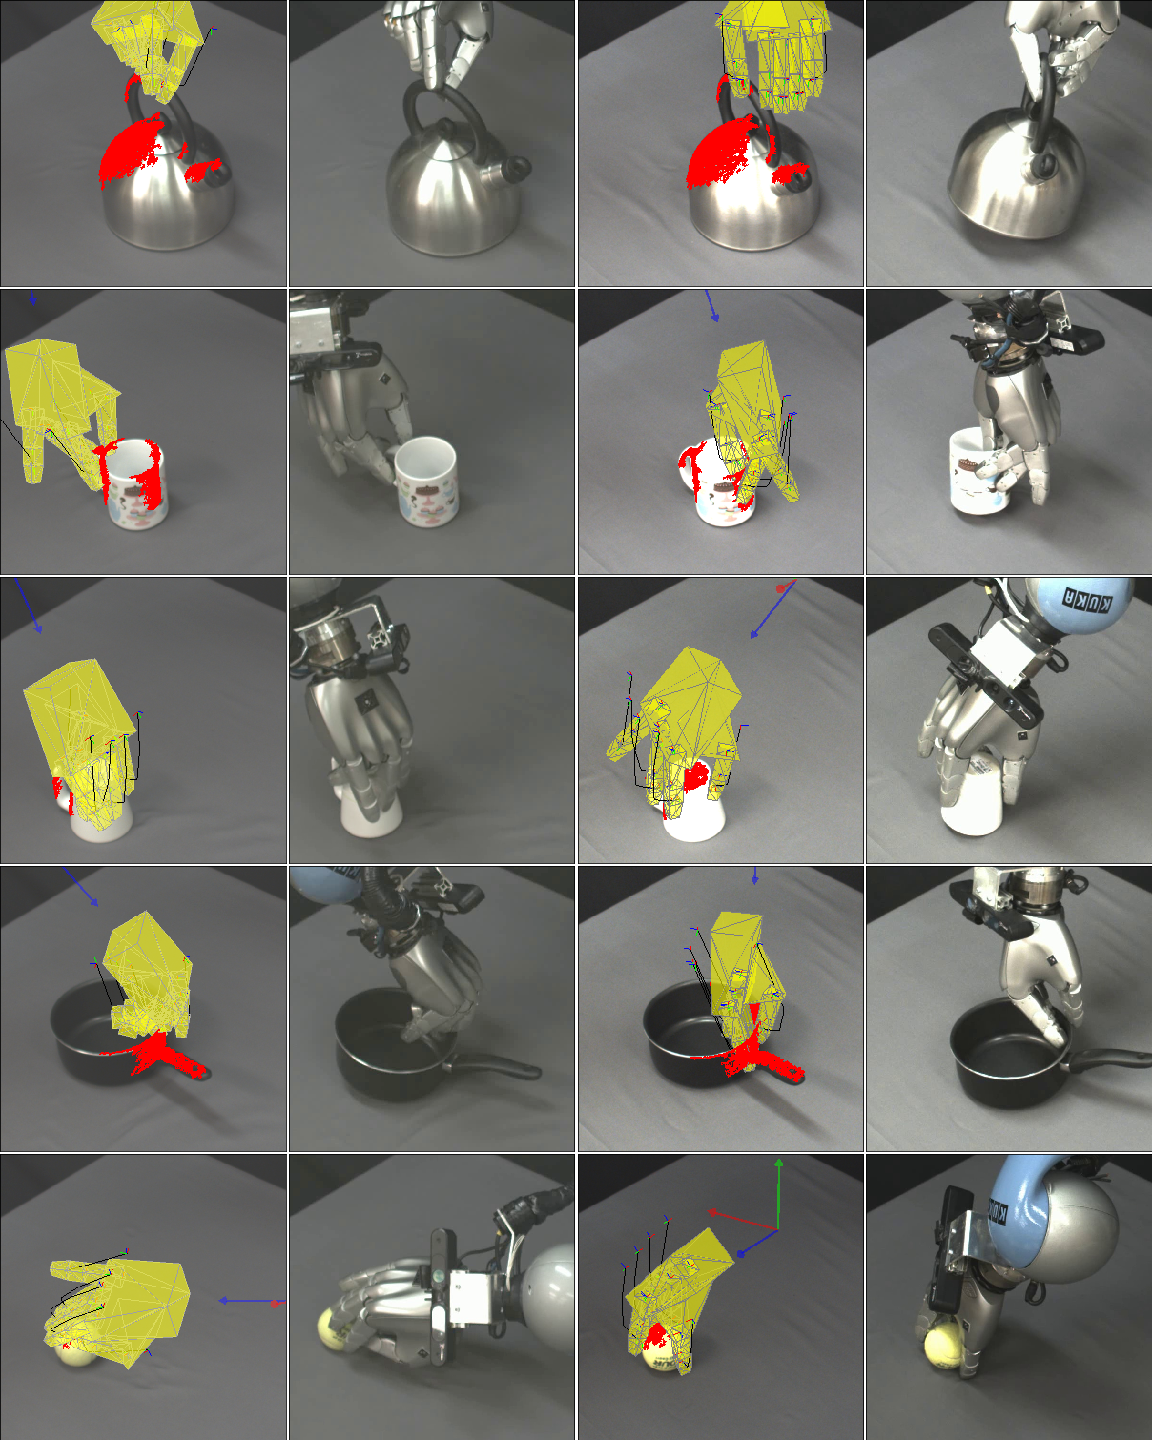
\includegraphics[width=0.5\columnwidth]{plots/A6fA10s_vertical.png}
\caption{V2 vs V11. This shows grasps from methods based on generative model GM2. The V2 grasps are shown in columns 1-2. The corresponding V11 grasps are shown in columns 3-4. These are the cases where V2 failed and V11 succeeded. \label{fig:v2fv11s}}
\end{center}
\end{figure}

\begin{figure}[t]
\begin{center}
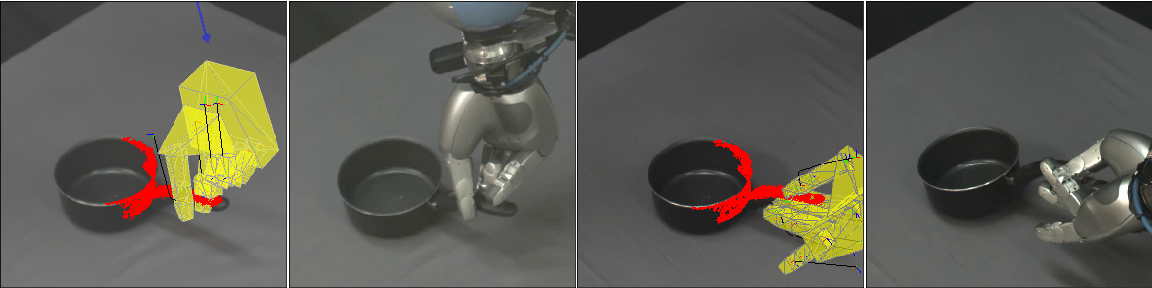
\includegraphics[width=0.5\columnwidth]{plots/A6fA10f_vertical.png}\\
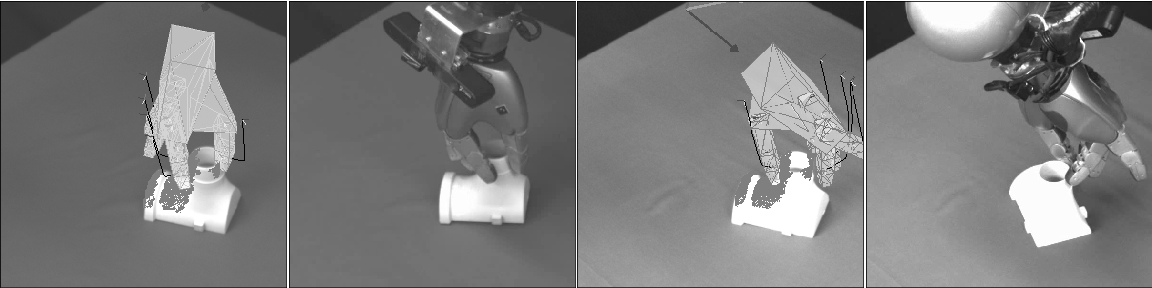
\includegraphics[width=0.5\columnwidth]{plots/A6sA10f_vertical.png}
\caption{V2 vs V11. This shows grasps from methods based on generative model GM2. The V2 grasps are shown in columns 1-2. The corresponding V11 grasps are shown in columns 3-4. The top row shows the case where both failed. The bottom row shows the case where V2 succeeded and V11 failed. \label{fig:v2fsv11f}}
\end{center}
\end{figure}


We compared four variants on the real robot: V1, V2, V4 and V11. V1 and V2 are the pure generative models. V4 is, in simulation, the equal best generative-evaluative method using GM1 as the generative model. It uses EM2 as the evaluative model. V11 is, in simulation, the best performing generative-evaluative method using GM2 as the generative model. This selection allows us to compare the best generative-evaluative methods with their counterpart pure generative models. 

We employed the same real objects as described in \cite{kopicki2019ijrr}. This used 40 novel test objects (Figure~\ref{fig:real-objects}). Object-pose combinations were chosen to reduce the typical surface recovery. Some objects were employed in several poses, yielding 49 object-pose pairs. From the 40 objects, 35 belonged to object classes in the simulation dataset, while the remaining five did not. 

Using this data-set, all algorithms were evaluated on the real-robot using a paired trials methodology. Each was presented with the same object-pose combinations. Each variant generated a ranked list of grasps, and the highest ranked grasp was executed. The highest-ranked grasp based on the predicted success probability of an evaluative network is performed on each scene. A grasp was deemed successful if, when lifted for five seconds, the object then remained stable in the hand for a further five seconds. 

The results are shown in Table~\ref{tab:robot-results}. In each case, the generative-evaluative variant outperforms the equivalent pure GM variant. So that V4 outperforms V1 by 75.5\% grasp success rate to 57.1\% and V11 outperforms V2 87.8\% to 81.6\%. The differences between V11:V1 and V2:V1 are highly statistically significant ($p<0.01$) using McNemar's test. Thus, we have strong support for our main hypothesis, which is that a Generative-Evaluative architecture outperforms a pure generative model. Six of the available grasp types were deployed (pinch support, pinch, pinchbottom, rimside, rim and power edge), showing that a variety of grasps is utilised.
%The success rate for GM1 was 57.1\% and for the top-performing method based on GM1, GEA.1, it was 77.6\% (Table~\ref{tab:robot-results}). The success rate of the second baseline, GM2, is 81.6\%, while GEA.3 shows outperforms it with a success rate of 87.8\%. A two-tailed McNemar test, for the difference between success rates for paired comparison data, was performed. The difference between the two algorithms has a $p$-value of 0.0442, and so is statistically significant. A selection of grasps where the two methods performed differently are shown in Figure~\ref{fig:successfail}.

% OLD TABLE
%\begin{table}
%\begin{center}
%\caption{Results of the real robot paired comparison trial.}
%\begin{tabular}{|c|c|c|c|}  \hline 
%          &                & \multicolumn{2}{ c |}{ GM} \\ \hline
%          &                & \# succs & \# fails  \\  \hline
 %GEA  & \# succs &  23 &  15  \\
 %         & \# fails    &  5   &   6   \\ \hline
%\end{tabular}
%\end{center}
%\label{tab:robot-results}
%\end{table}

%\begin{table}
%\begin{center}
%\caption{Results of the real robot paired comparison trial.}
%\label{my-label}
%\begin{tabular}{|cc|c|c|l}
%\cline{1-4}
%                                           &         & \multicolumn{2}{c|}{GM} &  \\ \cline{3-4}
%                                           &         & \# succs    & \# fails    &  \\ \cline{1-4}
%\multicolumn{1}{|c|}{\multirow{2}{*}{GEA}} & \# succs & 23         & 15         &  \\
%\multicolumn{1}{|c|}{}                     & \# fails & 5          & 6          &  \\ \cline{1-4}
%\end{tabular}
%\end{center}
%\label{tab:robot-results}
%\end{table}

\begin{figure*}
\begin{center}
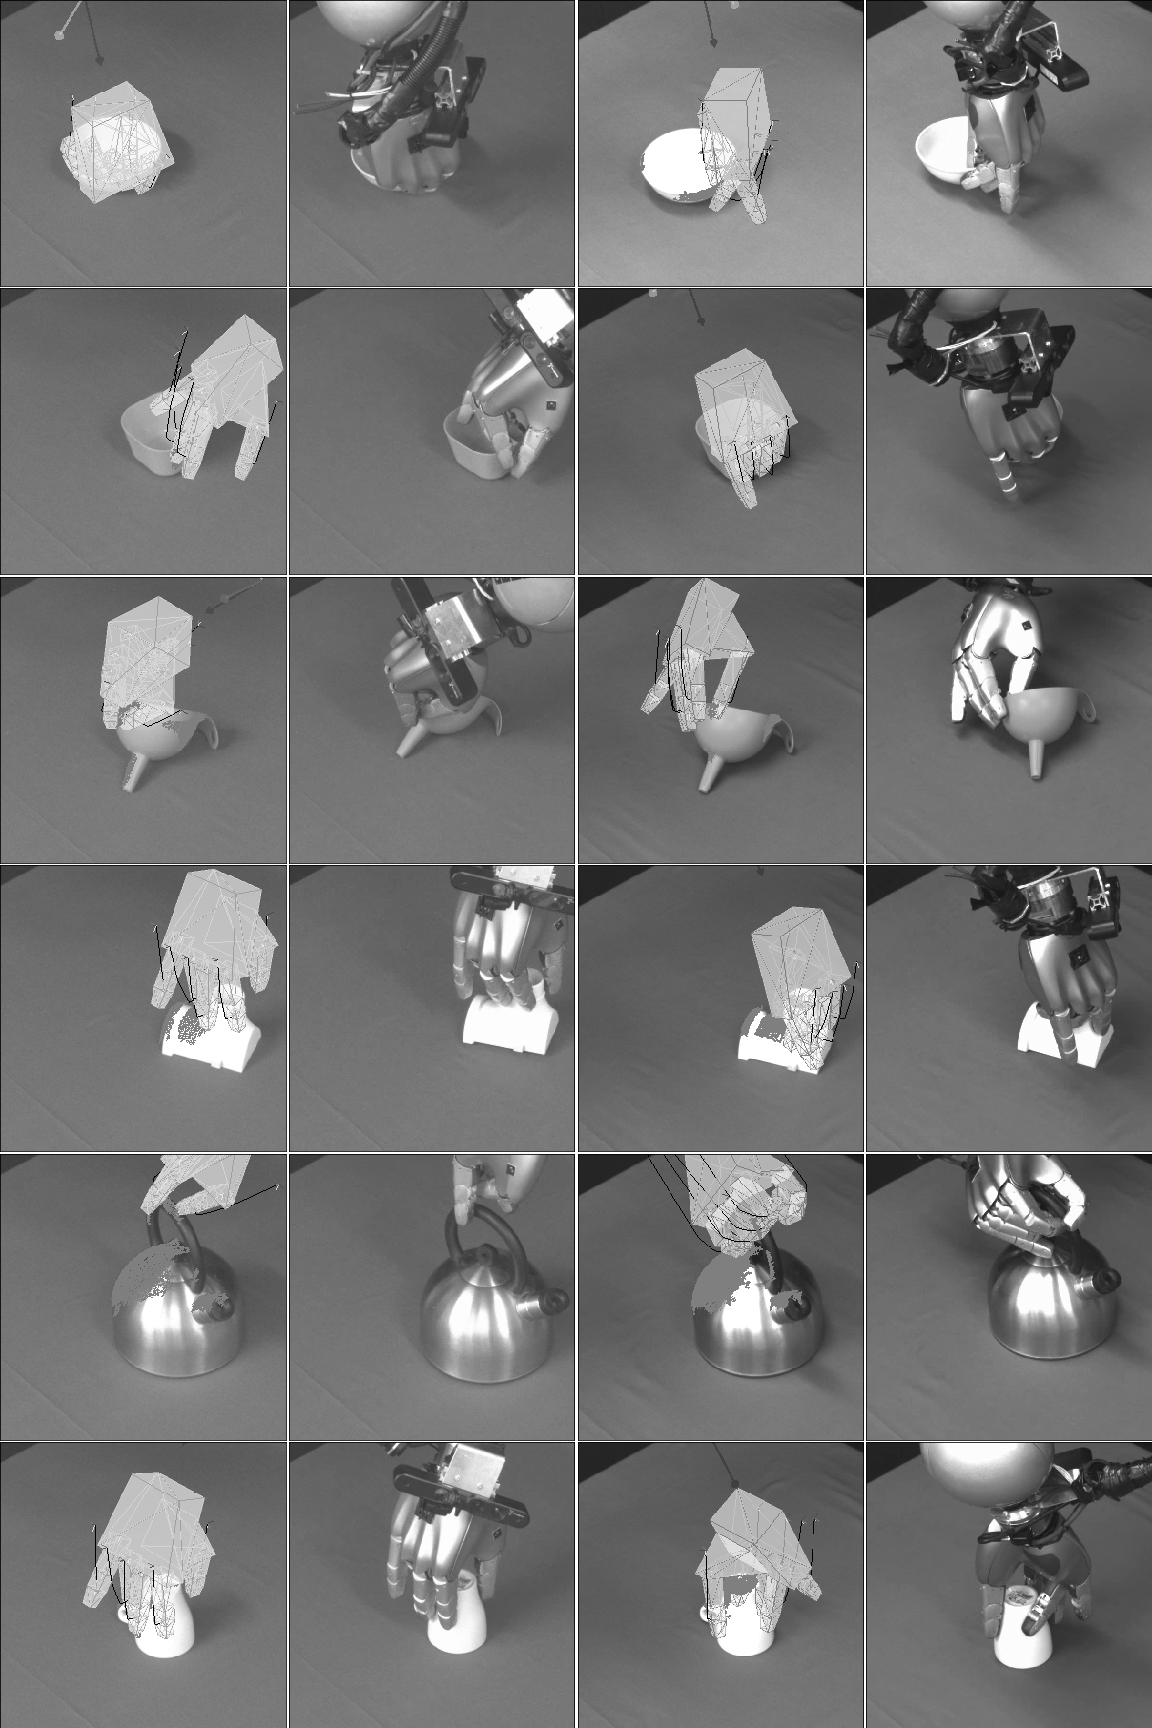
\includegraphics[width=0.48\textwidth]{plots/A2fA9s_1_vertical.png}~
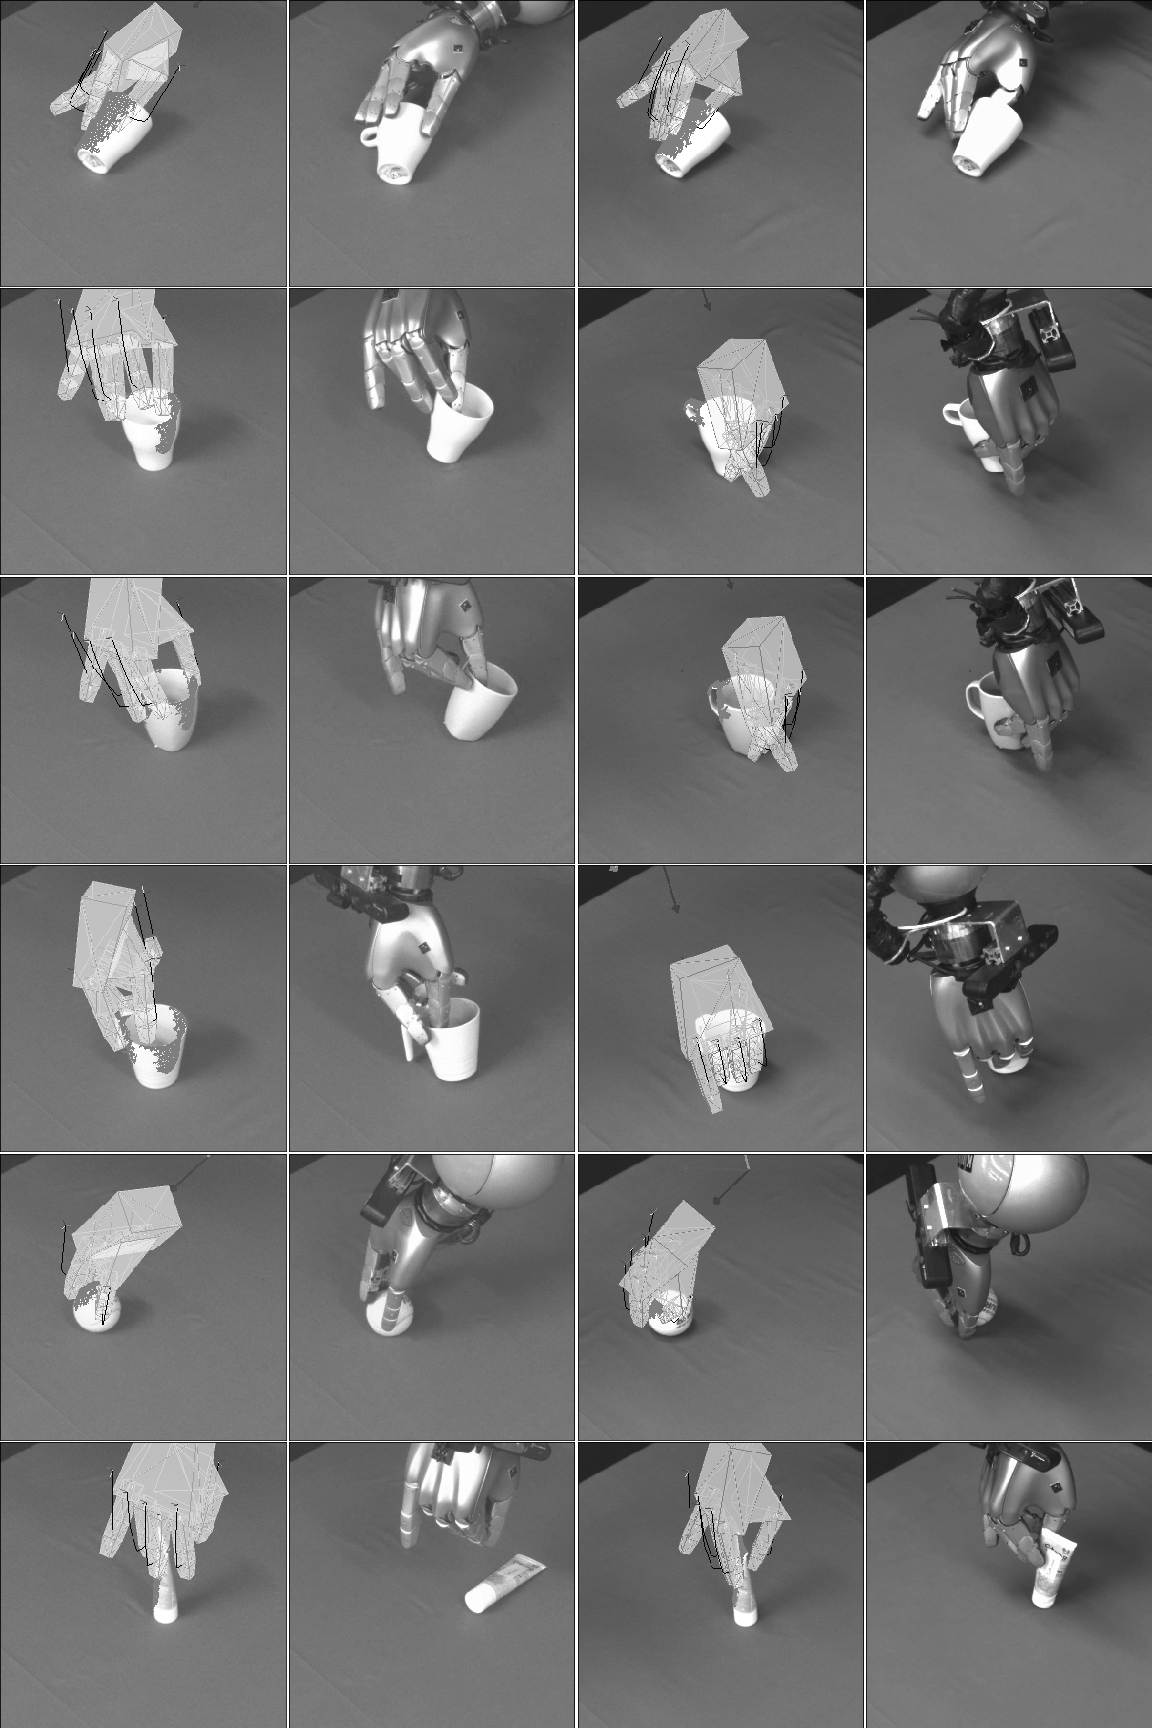
\includegraphics[width=0.48\textwidth]{plots/A2fA9s_2_vertical.png}
\caption{V1 vs V4. This shows grasps from methods based on generative model GM1. The V1 grasps are shown in columns 1-2 and 5-6. The corresponding V4 grasps are in columns 3-4 and 7-8. These are the cases where V1 failed and V4 succeeded.\label{fig:v1fv4s}}
\end{center}
\end{figure*}


\begin{figure*}
\begin{center}
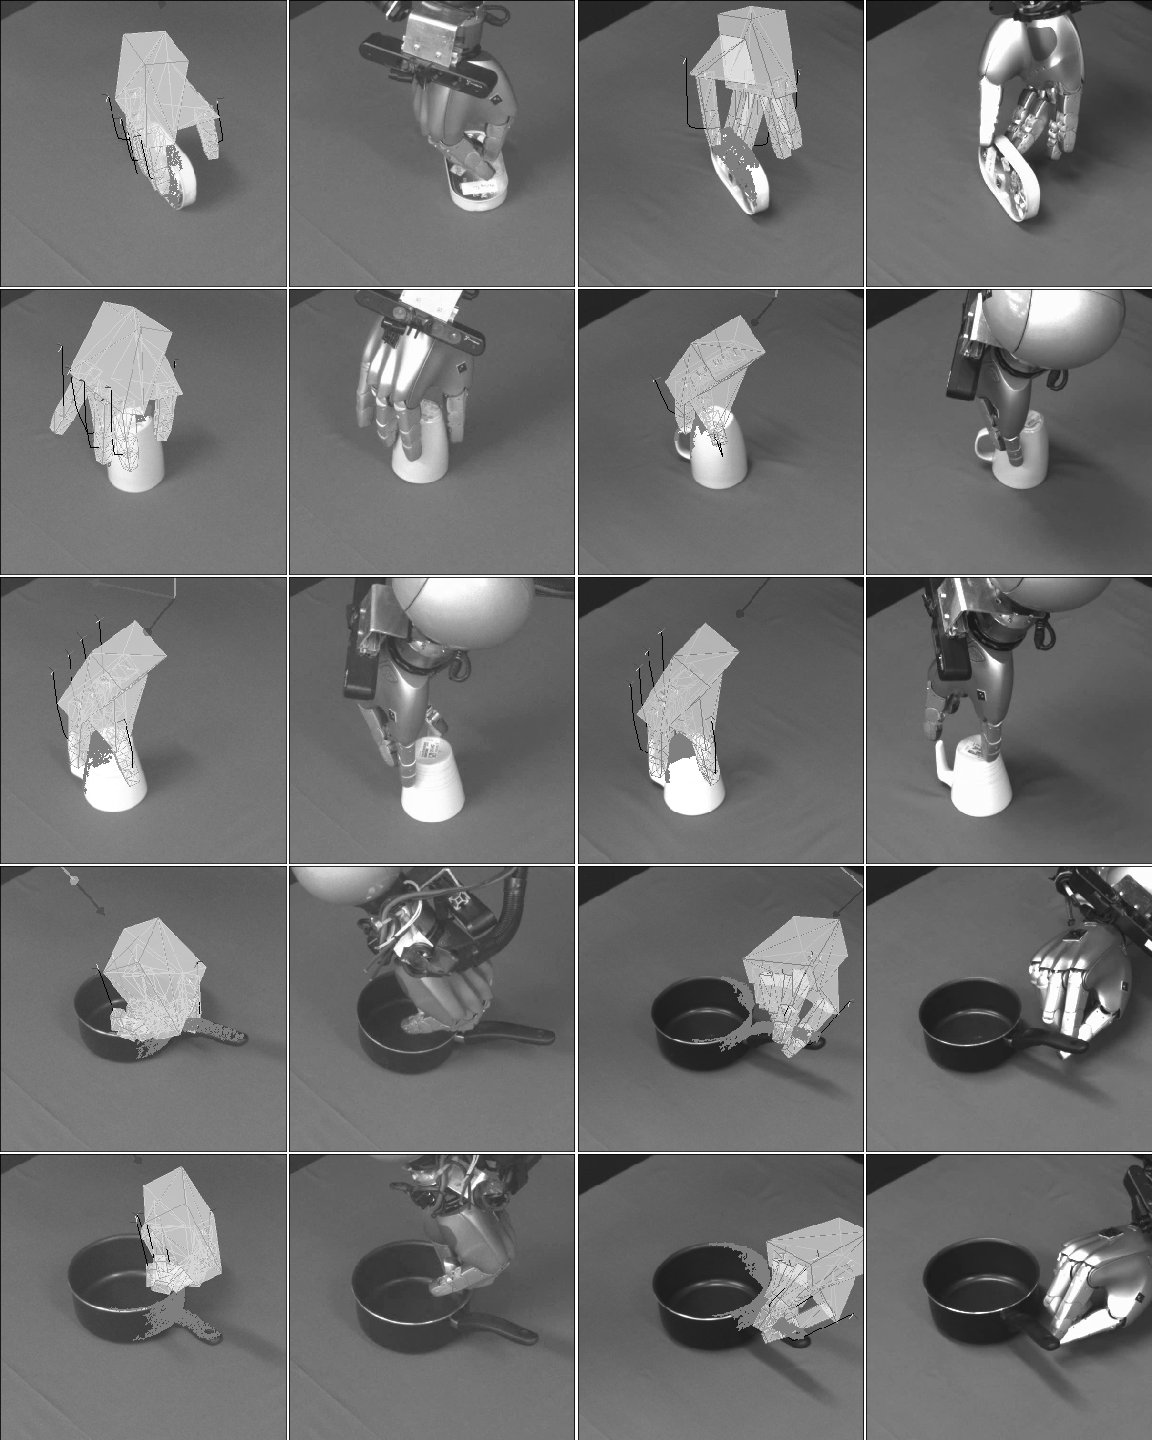
\includegraphics[width=0.48\textwidth]{plots/A2fA9f_vertical.png}~
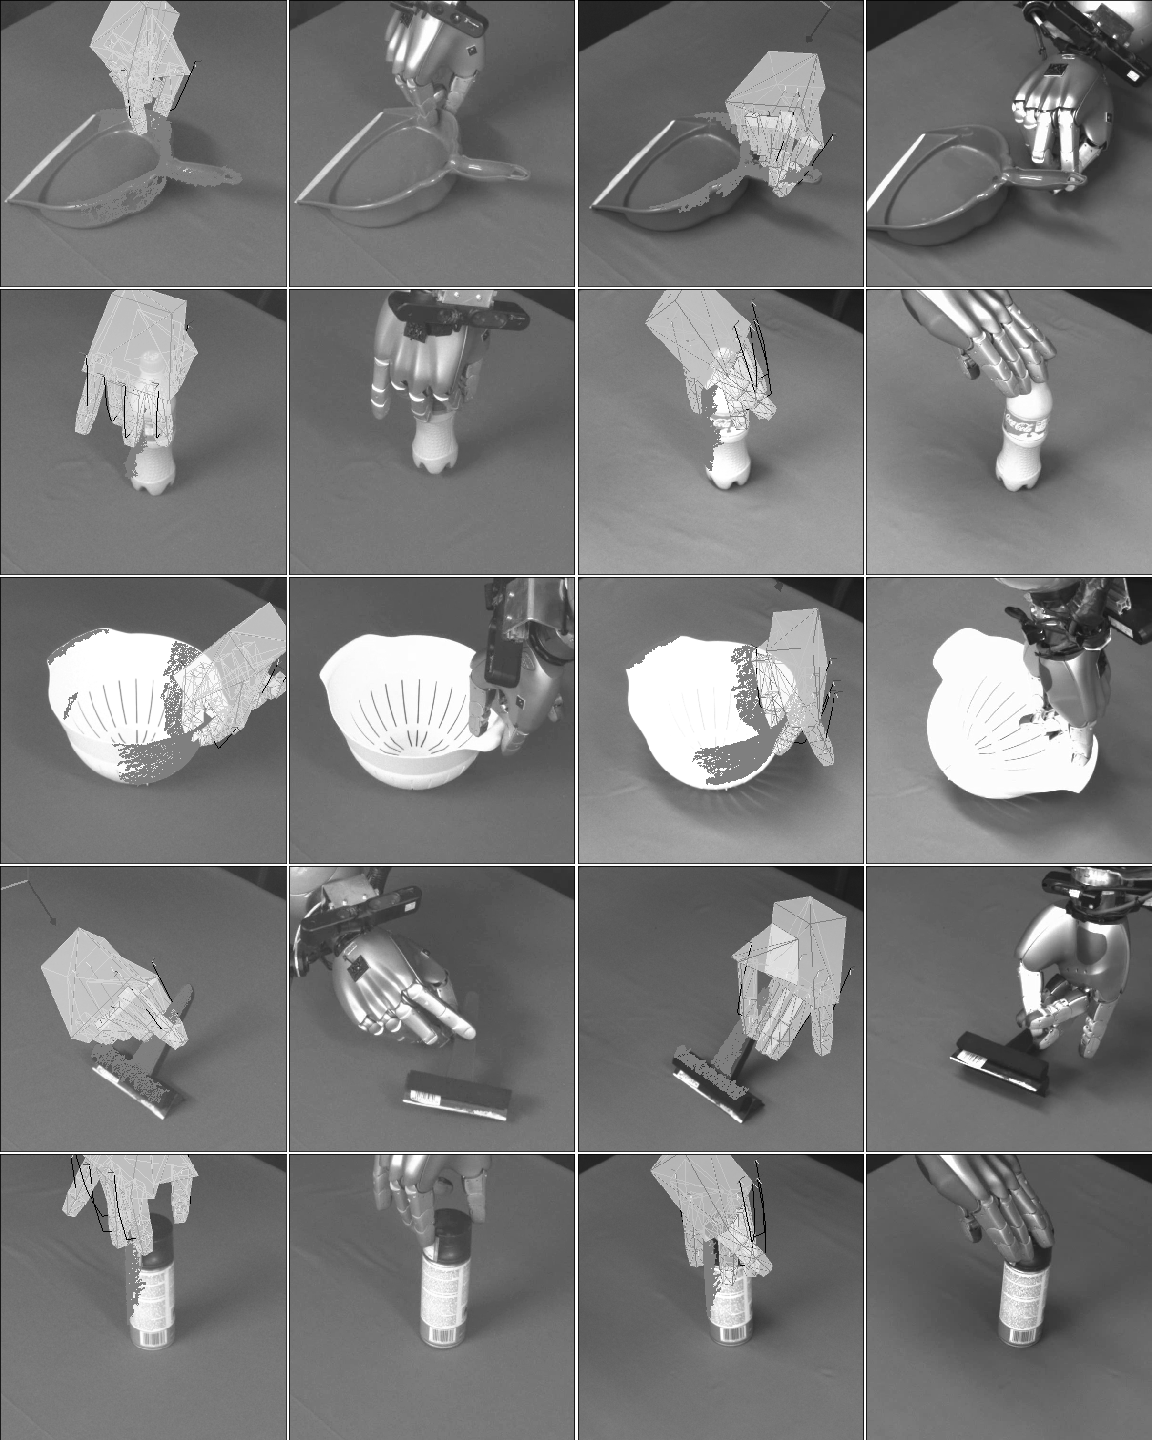
\includegraphics[width=0.48\textwidth]{plots/A2sA9f_vertical.png}
\caption{V1 vs V4. This shows grasps from methods based on generative model GM1. The V1 grasps are shown in columns 1-2 and 5-6. The corresponding V4 grasps are shown in columns 3-4 and 7-8. The left panel shows the cases where both V1 and V4 failed, while the right one shows the cases where V1 succeeded and V4 failed. \label{fig:v1fsv4f}}
\end{center}
\end{figure*}

%\begin{figure*}
%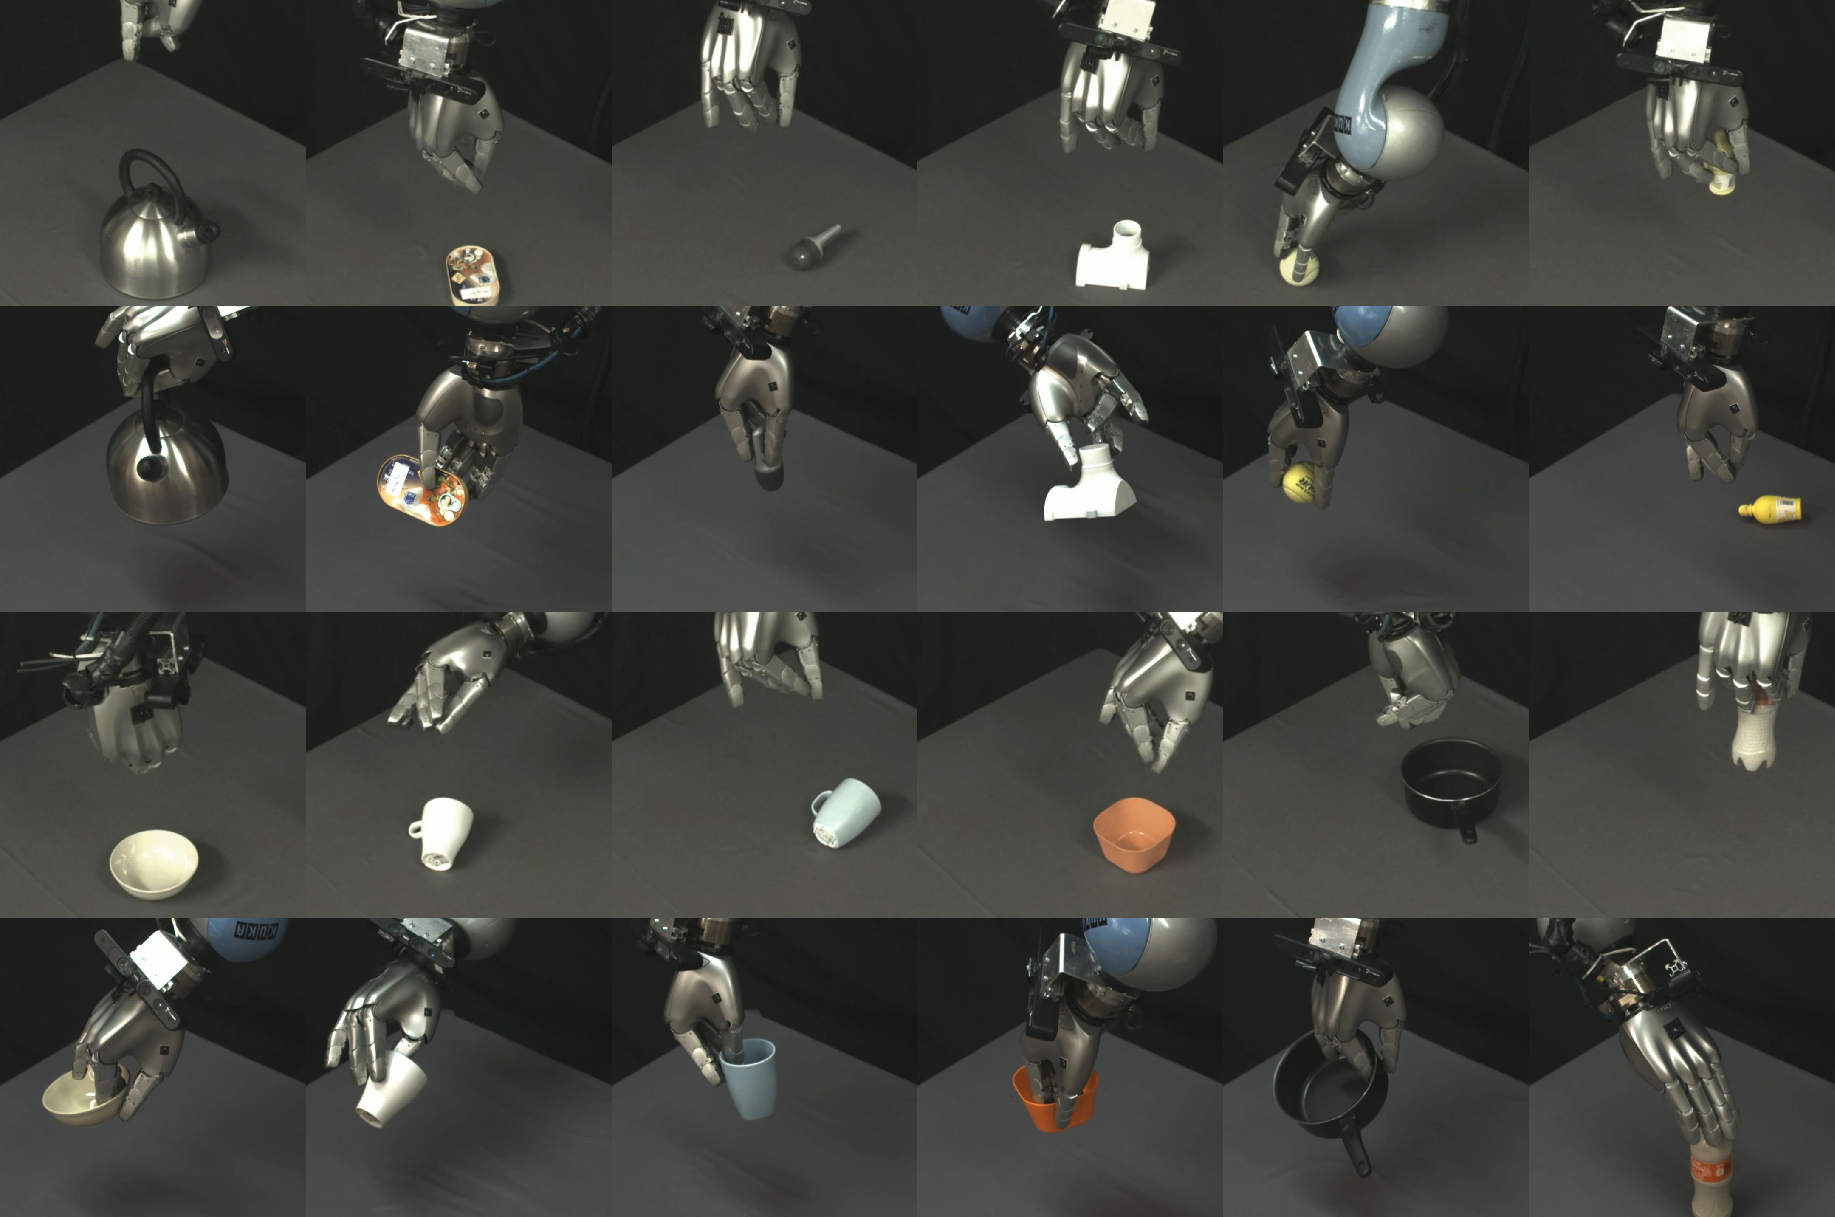
\includegraphics[width=\textwidth]{images/successfailure.pdf}
%\caption{Examples of grasps generated by the generative model (GM, $1^{st}$ and $3^{rd}$ row) and the generative-evaluative model (GEA, $2^{nd}$ and $4^{th}$ row) on paired trials. The first five columns show some of the 15 cases where the GEA model succeeds but GM fails. The far right-hand column shows 2 of the 5 converse cases. \label{fig:successfail}}
%\end{figure*}

%Training parameters for network. Training of example grasps for learning from demonstration. Creation of real test data set. Paired comparisons methodology with vanilla LFD algorithm (pose + object + camera view).
%
%The actual grasping tests have been performed on the real robot. 

\section{Extended Simulation Analysis}
\label{section:extendedSimulationAnalysis}

\noindent
This section analyses the behaviour of the best generative and evaluative models: V2 and V11 respectively. To perform this analysis we look at predictions on the DS2-Test set, which contains 124,137 grasps. %First, we would like to understand the statistics of the test data: how good are the grasps, are some grasps better than others? Second, we would like to know how well calibrated the evaluative model is, in other words we want to know how closely it predicts the grasp success probability. Third, we would like to know how much better the evaluative model is at ranking grasps than the initial ranking by the generative model. Finally, we want to how the evaluative model goes about improving performance, does it learn to re-rank grasp types or does it also do a good job of re-ranking grasps instances within a particular grasp-type?
%\subsection{How do grasp-type success rates vary?}
%\noindent
\begin{figure}[h]
\centering 
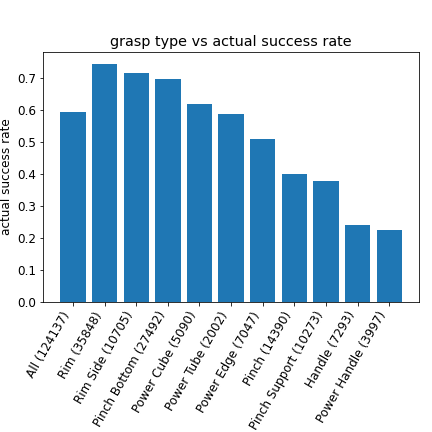
\includegraphics[width=0.5\columnwidth]{images/post-analysis/Grasp_type_vs_success_prob.png}
\caption{Grasp type vs. actual success rate.}
\label{fig:post2}
\end{figure}

%\subsection{How well are grasp success probabilities predicted?}
%\noindent
The first observation (Figure~\ref{fig:post2}) is that some grasp types are more likely to succeed than others. Grasp types with more finger links in contact with the object, such as Rim, Rim Side, or Power Cube have a higher success rate than those with fewer contacting links, such as Pinch and Handle.  This is due to the increased tolerance for finger positioning errors and the greater wrenches resisted when more contacts are made. 

The next question is how closely predicted success rates match the actual grasp success rates. Figure~\ref{fig:calibrate} is a histogram of successful (green) and unsuccessful (red) grasps in the test set. The historgram is organised on the horizontal axis by the predicted grasp success probability according to V11. The vertical axis shows the proportion of grasps that were actually successful. The closer the blue line is to the straight line showing perfect calibration, the better the prediction of the probability of success. When we aggregate all grasp-types, this prediction is close to perfect. The correlation also holds, though more weakly, when broken out across grasp types. \footnote{Where there is little data in the test set we plot the 95\% confidence interval for actual grasp success rate. Where the confidence interval is large we cannot draw a strong conclusion about the predictive power. It is noteworthy that the major deviations from perfect calibration are in areas with little data.}
%This suggests that V11 performance in the real robot experiments could be further improved by employing multiple views of the same object until a grasp is found where the network is highly confident that the grasp will succeed. Applying such an algorithm is beyond the scope of this paper, where the restrictions limits us to one view per object to generate grasps.

\begin{figure}[h]
\centering
\includegraphics[width=1.02\columnwidth]{images/post-analysis/V11_pred_success_vs_success.png}
\caption{Predicted success probability vs actual success probability for V11. The red bars indicate failures, and green bars show successes. The grasps are ordered along the horizontal axis by the predicted success probabilities of EM3. The blue line shows the (actual) average success rate of grasps in every bin, while the height of the shaded blue region is the standard error of the actual success rates in nearby bins. When there are insufficient grasps to estimate actual success rates (Handle and Power Tube), the uncertainty increases significantly.}
\label{fig:calibrate}
\end{figure}

%\subsection{How much better is the evaluative model's grasp ranking?}
%\noindent
The next question is how much better the evaluative model in V11 is than the generative model V2 in ranking grasps. The generative and evaluative models each produce a number for each grasp. This is a likelihood for the generative model (GM2) and a predicted probability of success for the evaluative model (EM3). These numbers are used to rank all the grasp-scene pairs in the test set. For a perfect ranking, all the successful grasps must be ranked above all the unsuccessful grasps. We can visualise the quality of each ranking using an ROC curve (Figure~\ref{fig:roc}). The metric used to compare different models is the area under the curve (AUC). This metric is calculated for each scene and averaged across all scenes in the test set. It can be seen that V11 improves on V2 in separating successful from unsuccessful grasp instances for every grasp type. It also improves overall. The AUC across all grasps increases from 0.71 (V2) to 0.9 (V11). 

\begin{figure}[h]
\centering
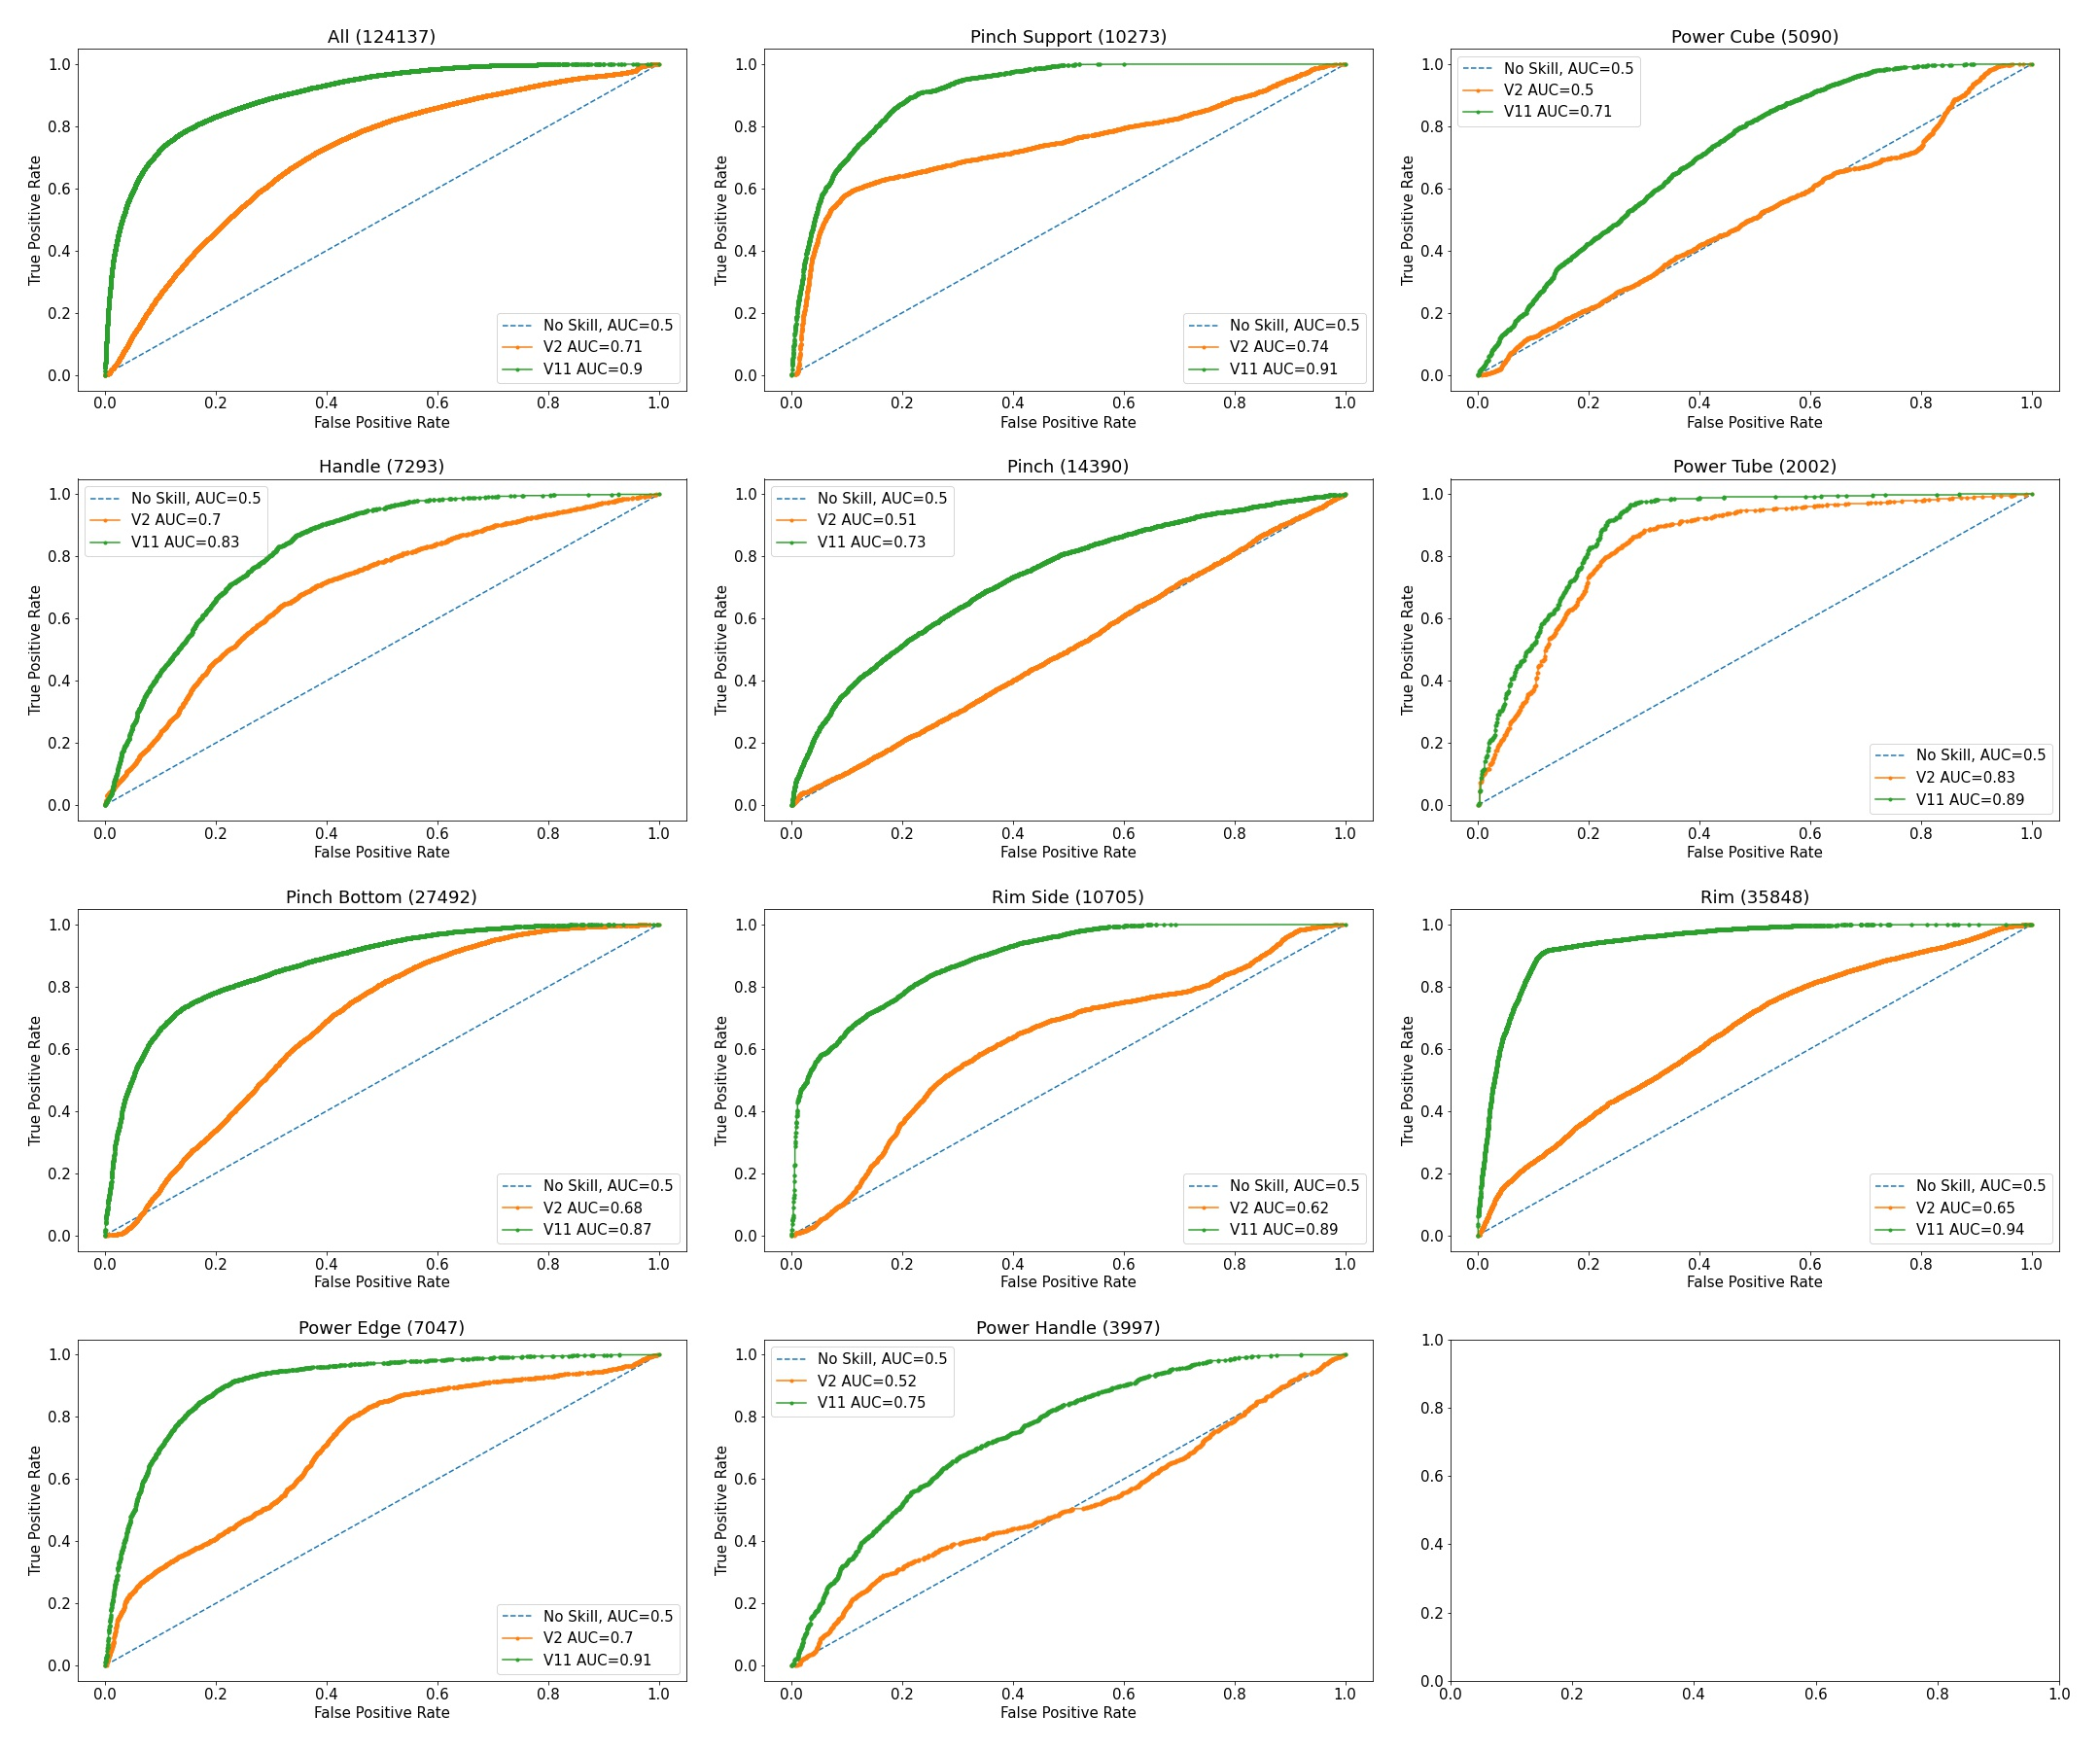
\includegraphics[width=1.0\columnwidth]{images/post-analysis/roc-analysis}
\caption{\label{fig:roc}ROC curves for the evaluative model in V11 (EM3) and the underlying generative model (GM2/V2).}
\end{figure}

This analysis also shows that V11 successfully re-ranks grasps within a grasp type. Does the model also rank better than V2 between the grasp types? This can be answered by looking at the how much a method (V2 or V11) shifts up or down the average ranking of a grasp type relative to a random ranking. We calculate this shift for both V2 and V11 and then look at the correlation between this shift and the grasp-type success rate (Figure~\ref{fig:v2_vs_v11_rates}). This shows that both V2 and V11, on average, shift up grasp types that are more likely to be successful and shift down grasp types that are less likely to be successful. So, although the rankings are of grasp instances, we see that the effect is that information about the success rate of grasp types is also encoded. The Pearson correlation coefficient between V11's average improvement rates and actual success rates is 0.94, while V2's coefficient is 0.69.

%V11, which combines the generative model GM2 with the evaluative model EM3, yields a substantial improvement over GM2's ranking, improving GM2's simulation top-grasp success rate from 79.05\% to 90.49\%, and real-world performance from 81.6\% to 87.8\%. We hypothesise that two main factors could contribute to this result. First, EM3 could be assigning high predicted success probabilities to grasp types that are generally successful, and low probabilities to those grasp types that fail often. Effectively, this would mean that a ranking based on EM3's predicted probabilities would simply be favouring grasp types that are, on average, more successful than others. Second, within each grasp type, EM3 may be learning which approach trajectories and hand/finger positions are more likely to be successful with respect to the object. The second hypothesis is more interesting. Such evidence would imply that the network is learning to associate the object's geometry with the approach trajectory and configuration. Below, we look for evidence to support both factors.

%\subsubsection{Does the evaluate model learn to rank grasp types?}
%\noindent

%\begin{figure}
%\centering
%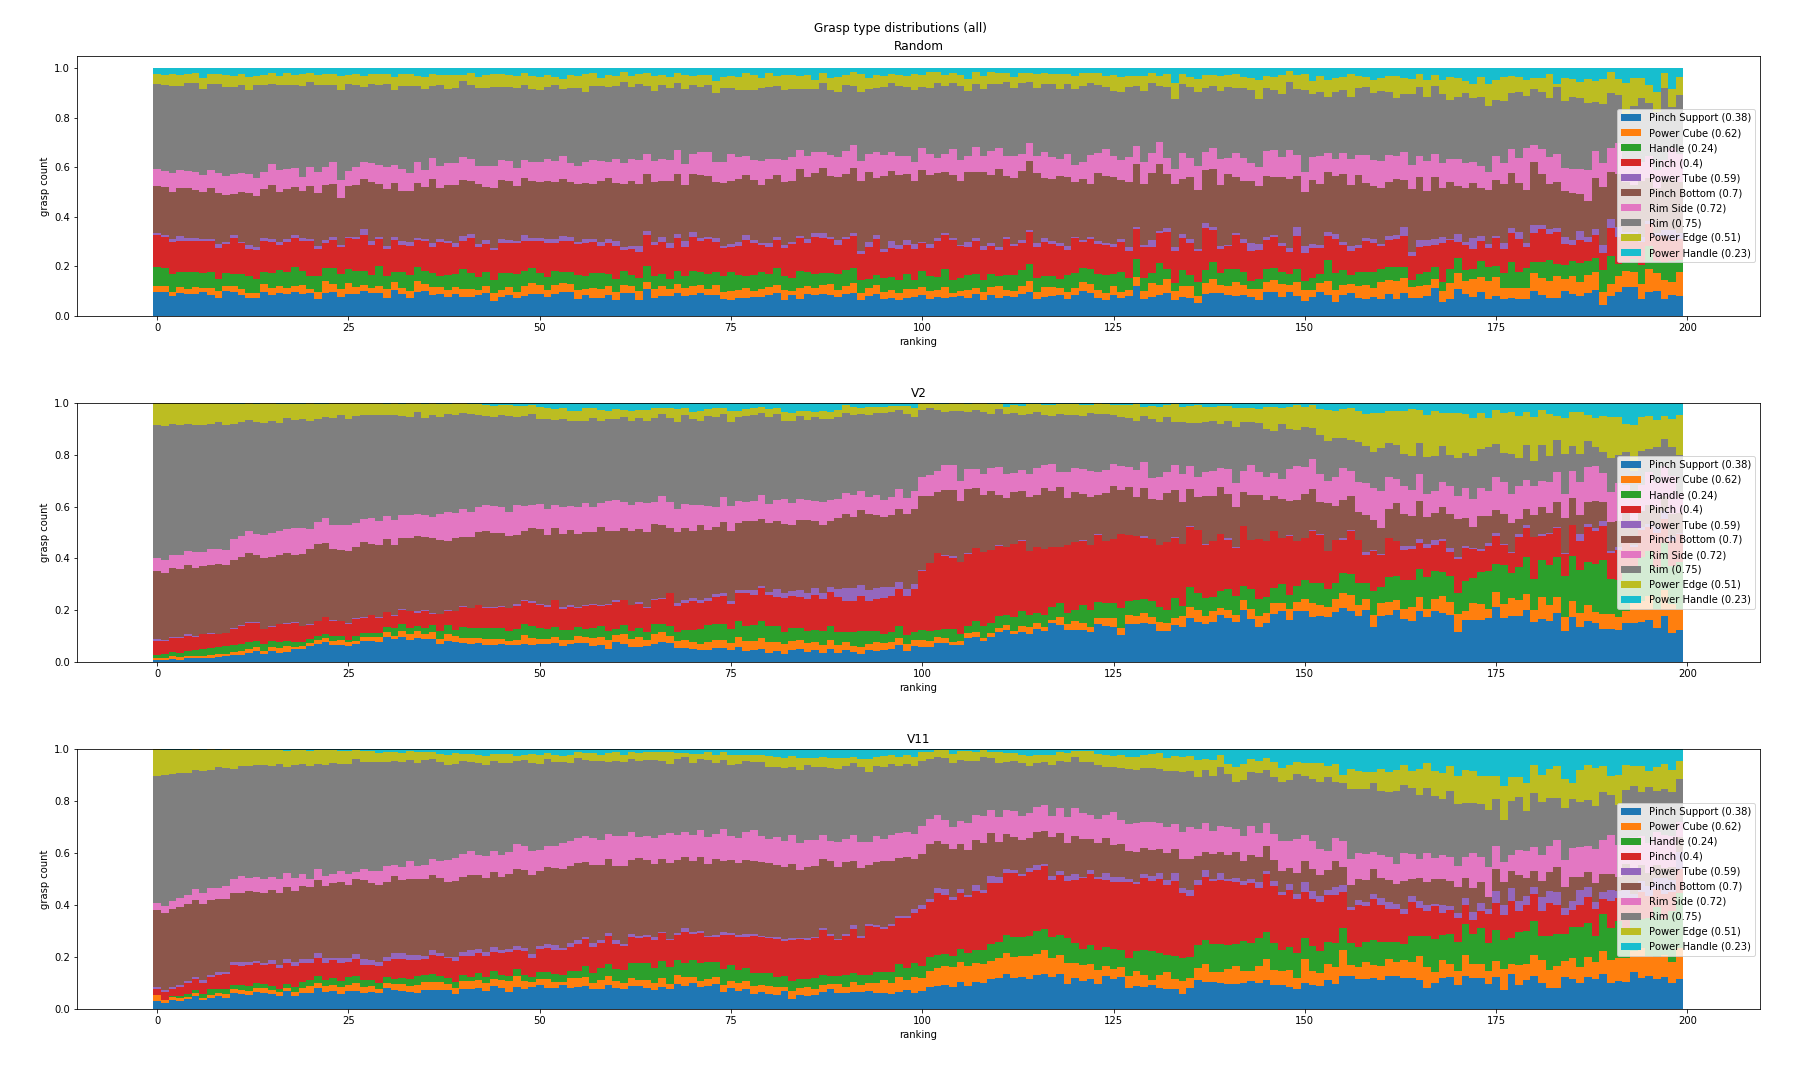
\includegraphics[width=0.8\columnwidth]{images/post-analysis/Grasp_type_distributions_all.png}
%\caption{Comparison of grasp type distributions per ranking of random, V2 and V11 rankings.}
%\label{fig:post6}
%\end{figure}

\begin{comment}
\begin{table}[h]
\small
\centering
\begin{tabular}{llll}
\hline
Grasp Type & Random Rank. & V2 Rank.  & V11 Rank.\\ \hline
Pinch Support & $\mathbf{97.4} \pm 82.8$  & $\mathbf{120.3} \pm 75.9 [\mathbf{+22.9}]$ & $\mathbf{111.9} \pm 78.6 [\mathbf{+14.5}]$ \\ \hline
Power Cube & $\mathbf{135.7} \pm 100.3$  & $\mathbf{162.4} \pm 92.1 [\mathbf{+26.7}]$ & $\mathbf{132.9} \pm 83.1 [\mathbf{-2.8}]$ \\ \hline
Handle & $\mathbf{97.2} \pm 83.3$  & $\mathbf{156.5} \pm 97.7 [\mathbf{+59.3}]$ & $\mathbf{149.5} \pm 86.2 [\mathbf{+52.3}]$ \\ \hline
Pinch & $\mathbf{87.1} \pm 72.7$  & $\mathbf{111.4} \pm 71.7 [\mathbf{+24.3}]$ & $\mathbf{104.5 }\pm 63.6 [\mathbf{+17.4}]$ \\ \hline
Power Tube & $\mathbf{121.0} \pm 92.5$  & $\mathbf{213.4} \pm 107.6 [\mathbf{+92.4}]$ & $\mathbf{118.7} \pm 82.6 [\mathbf{-2.3}]$ \\ \hline
Pinch Bottom & $\mathbf{89.8} \pm 69.5$  & $\mathbf{71.0} \pm 60.4 [\mathbf{-18.8}]$ & $\mathbf{75.6} \pm 77.9 [\mathbf{-14.2}]$ \\ \hline
Rim Side & $\mathbf{107.6} \pm 89.6$  & $\mathbf{91.6} \pm 69.2 [\mathbf{-16.0}]$ & $\mathbf{115.9} \pm 83.6 [\mathbf{+8.3}]$ \\ \hline
Rim & $\mathbf{85.9} \pm 76.5$  & $\mathbf{61.5} \pm 54.6 [\mathbf{-24.4}]$ & $\mathbf{66.3} \pm 60.8 [\mathbf{-19.6}]$ \\ \hline
Power Edge & $\mathbf{125.0} \pm 98.5$  & $\mathbf{102.9} \pm 81.7 [\mathbf{-22.1}]$ & $\mathbf{123.4} \pm 99.4 [\mathbf{-1.6}]$ \\ \hline
Power Handle & $\mathbf{121.0} \pm 95.7$  & $\mathbf{216.1} \pm 106.3 [\mathbf{+95.1}]$ & $\mathbf{184.5} \pm 99.1 [\mathbf{+63.5}]$ \\ \hline
\end{tabular}
\caption{Changes in average grasp position per grasp type according to Random, V2 and V11 rankings.}
\label{table:rankingchanges}
\end{table}
\end{comment}

\begin{figure*}[h]
\begin{center}
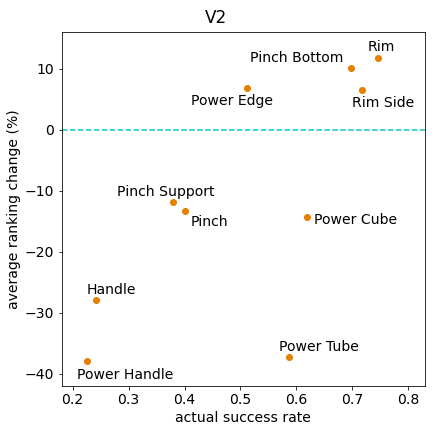
\includegraphics[width=0.35\textwidth]{images/post-analysis/V2_suc_rate_vs_improvement.png}~
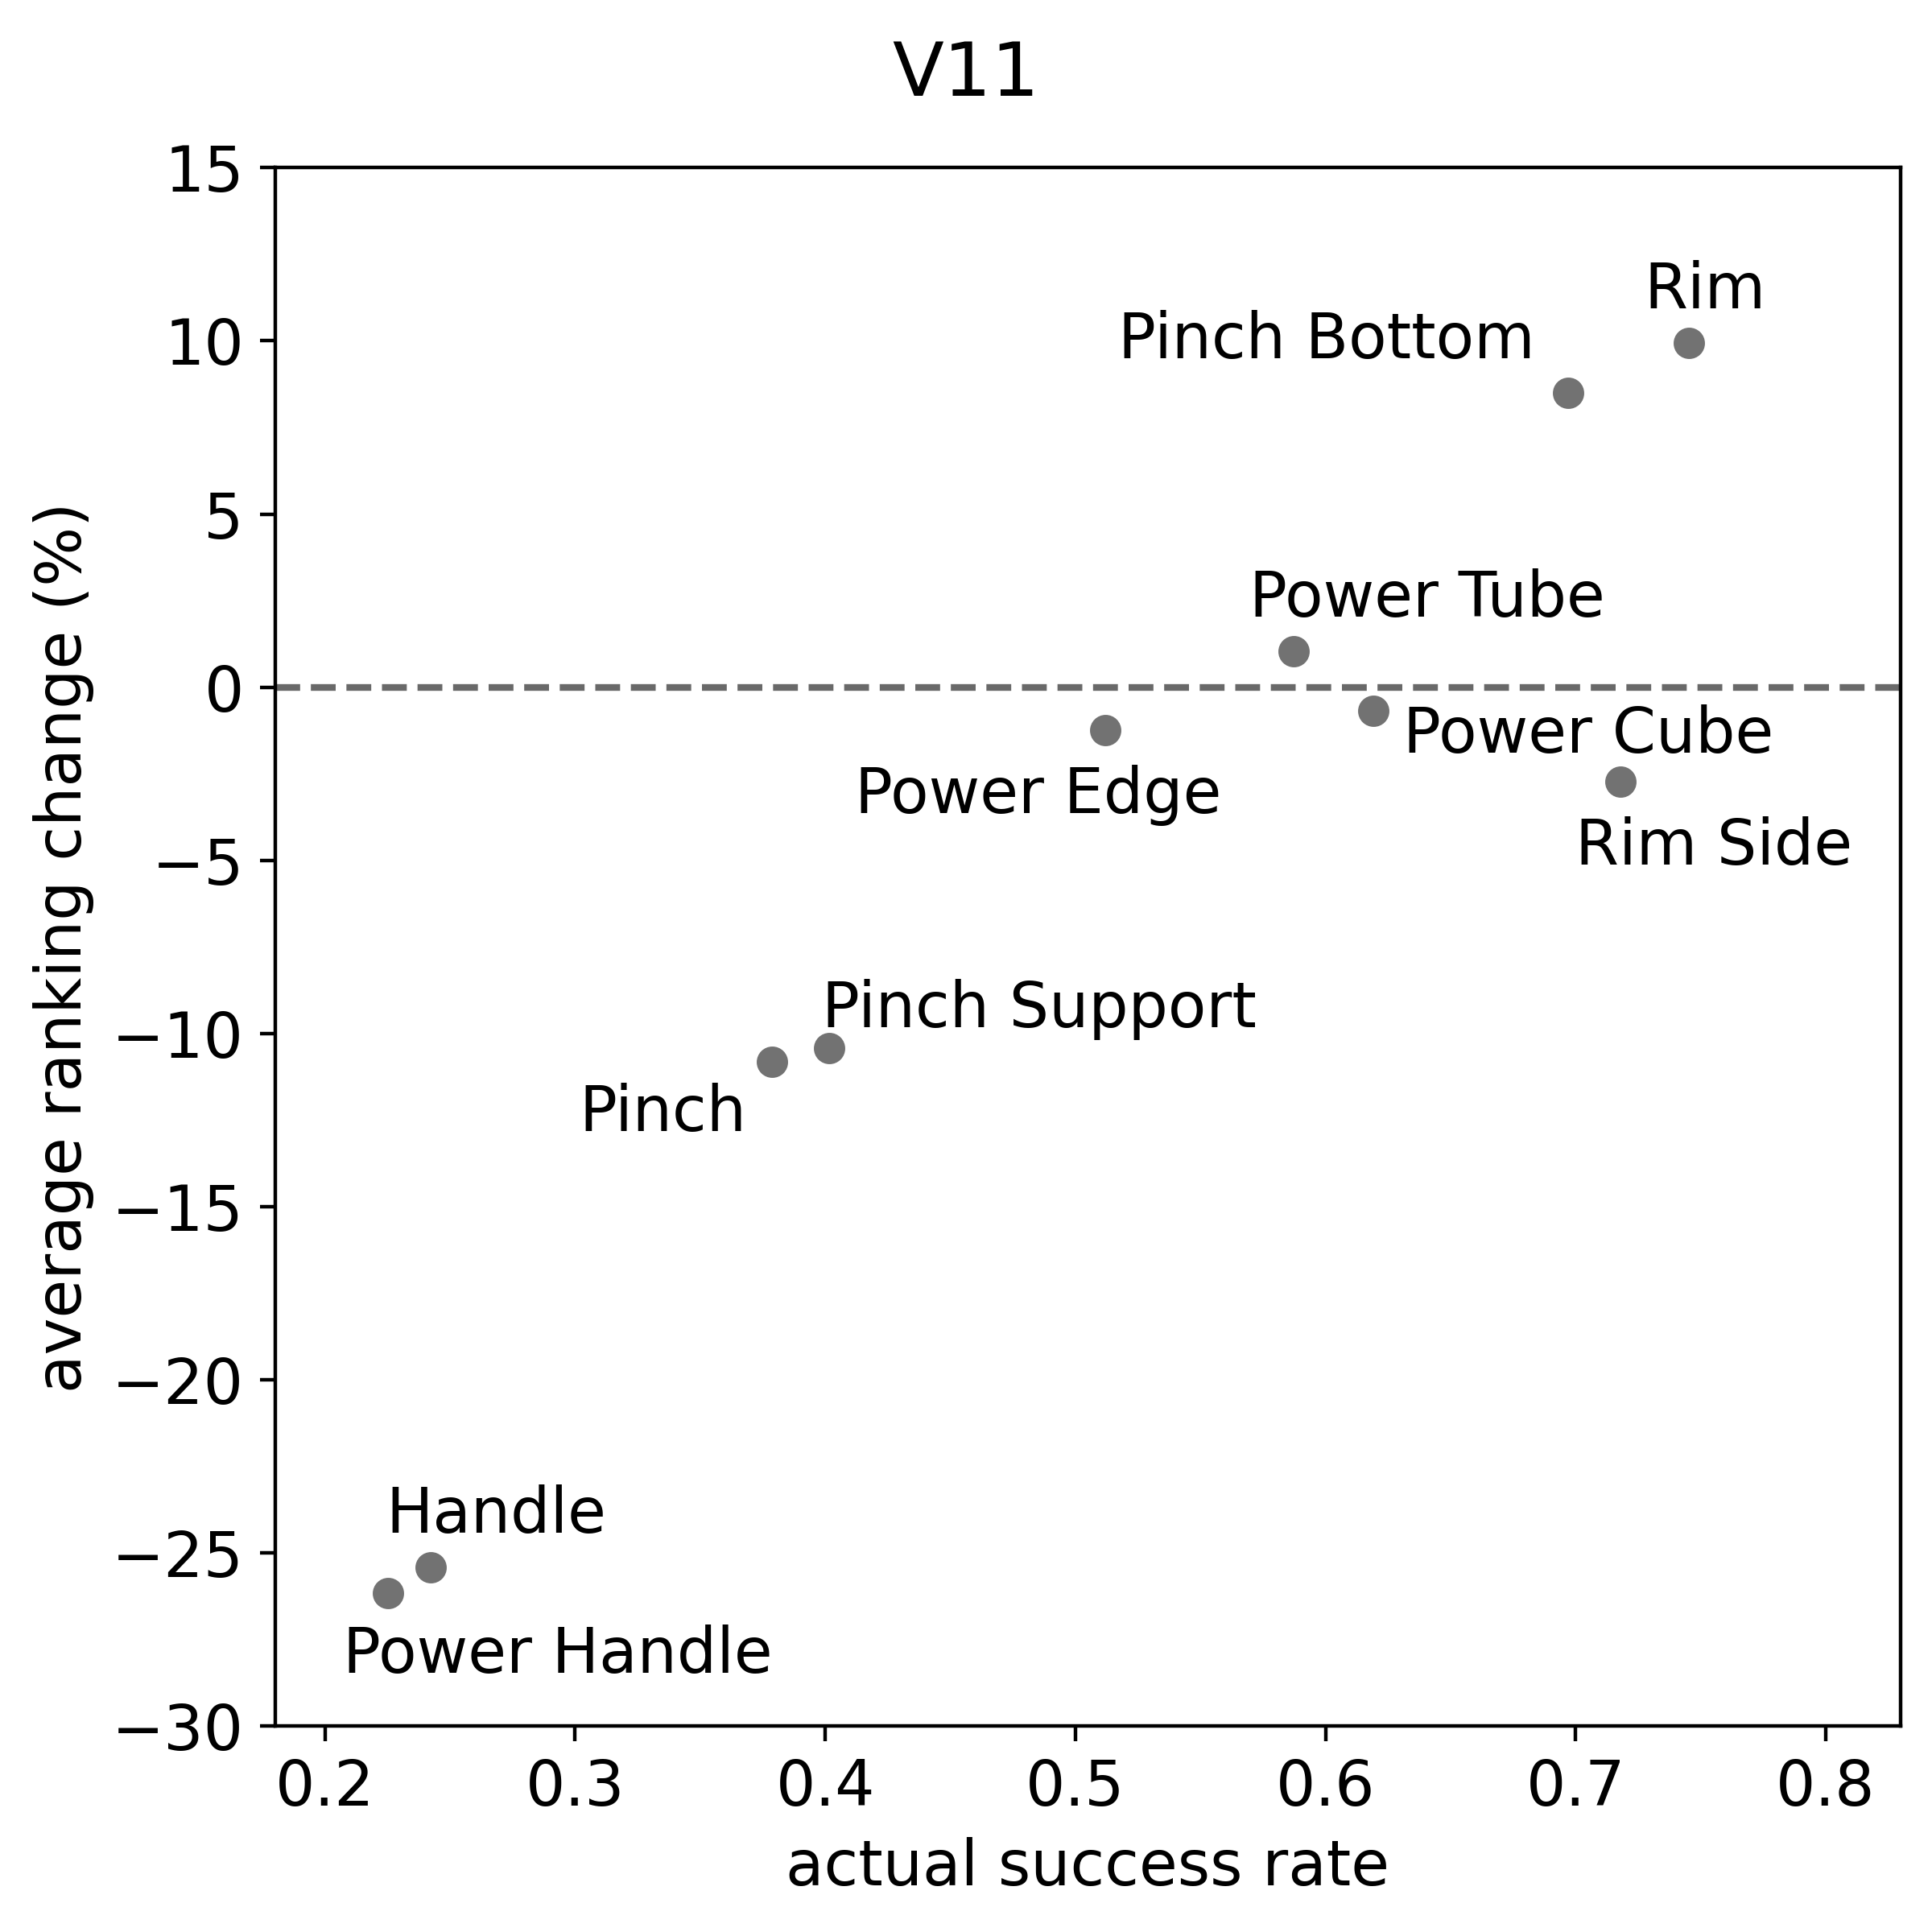
\includegraphics[width=0.35\textwidth]{images/post-analysis/V11_suc_rate_vs_improvement.png}
\caption{Comparing the per-grasp type average ranking improvement of V2 and V11, with random ranking taken as reference. Average ranking improvement is the average shift (\%) of all examples of a grasp type in a scene, aggregated across all test scenes where that grasp type is present. V11's shifts correlated with actual grasp success rates yield a Pearson coefficient of 0.94, while V2 achieves 0.69. \label{fig:v2_vs_v11_rates}}
\end{center}
\end{figure*}


%Figure~\ref{fig:v2_vs_v11_rates} compares the per-grasp type average ranking improvement of V2, which is based on the generative model GM2, and V11, which employs evaluative model EM3. Both are calculated by taking the random ranking, which are based on randomly assigned success probabilities, as reference. Both V2 and V11 appear to favour robust grasps over that fail more often, despite calculating the grasp success probabilities in entirely different ways. The Pearson correlation coefficient between V11's average improvement rates and actual success rates is 0.94, while V2's coefficient is only 0.69. While a causal link is yet to be established, V11 ranking's strong correlation with per-grasp-type success rates suggests V11 (therefore EM3) learns to rank grasps according to their grasp types.

%\begin{figure}
%\centering
%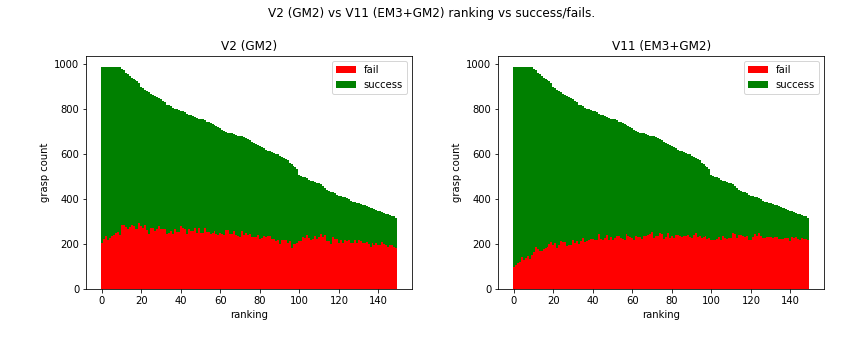
\includegraphics[width=0.8\columnwidth]{images/post-analysis/[3] V2_vs_V11_ranking_vs_success_fail.png}
%\caption{Comparison of successful (green) and unsuccessful (red) grasps per ranking for V2 and V11.}
%\label{fig:post3}
%\end{figure}

%\subsubsection{Does EM3 rank grasps within a grasp type?}
%\noindent

%The second hypothesis we have is that EM3 is learning to rank grasps within each grasp type, favouring grasp trajectories that are more likely to be successful over others. In order to test this hypothesis, we compared three different strategies above: random, V2, V11. In Figure~\ref{fig:post5}, we compare the the quality of the ranking of grasps within each grasp type. In order to compare rankings, a grasp's ranking, multiplied by -1, is used as the classification score in a binary classification problem (failure/success). The metric used to compare different models is the area under Receiver Operating Characteristics (ROC) curve. This metric is calculated for each scene, and averaged across all scenes in the test set. The left-most plot in Figure~\ref{fig:post5} shows that the overall ranking quality of V11 is better than V2 and random predictions across grasp types. Furthermore, V11 has the best overall within-type ranking for all grasp types except for Power Tube. This observation suggests that V11 not only leans on the grasp type information, but also learns to associate the object's geometry with the grasp trajectories to determine whether a grasp will be successful.

%\begin{figure}[h]
%\centering
%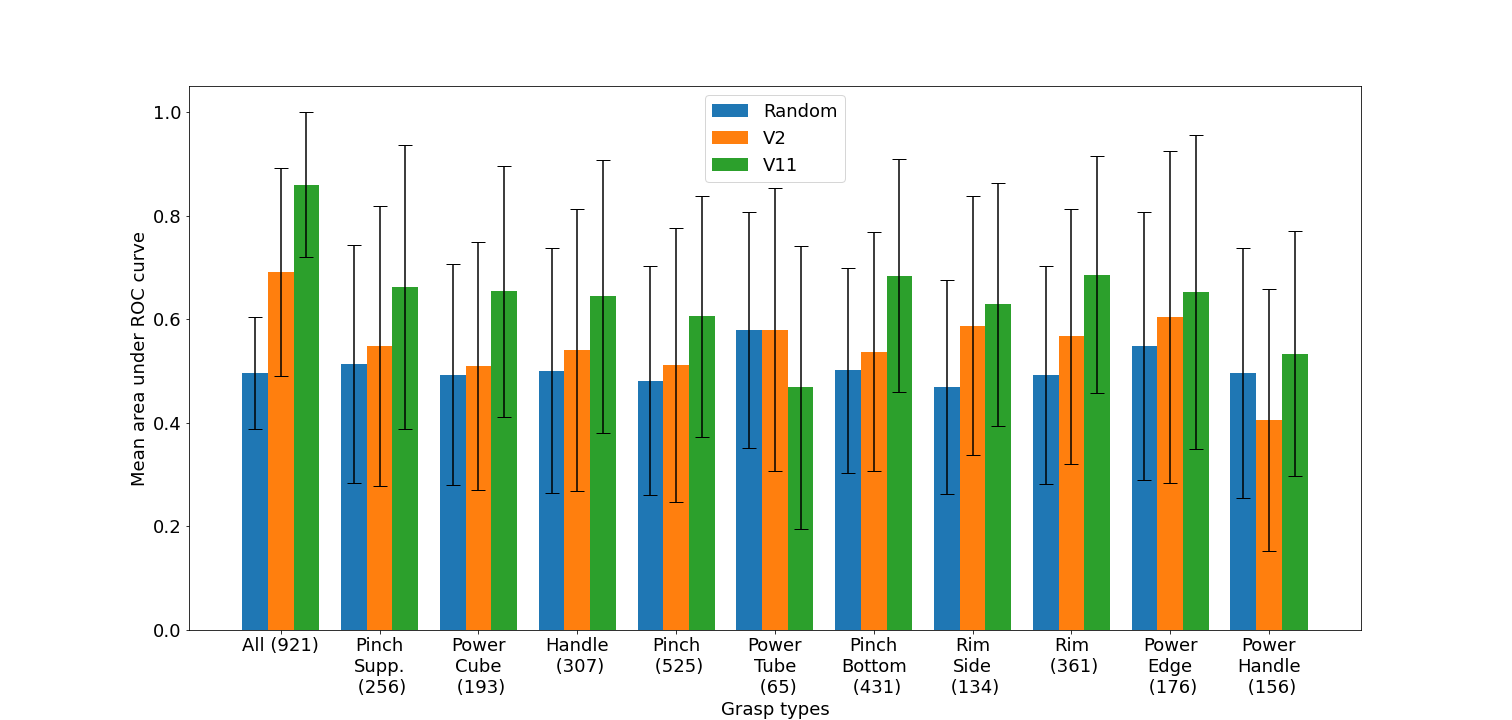
\includegraphics[width=0.999\columnwidth]{images/post-analysis/Ranking_quality_mean_AUC.png}
%\caption{Within-type grasp ranking quality comparison of random, V2 and V11 predictions according to the Area-Under-Curve of Receiver Operating Characteristics (AUC-ROC) metric. Higher score is better. V11's ranking outperforms those of random and V2, except for Power Tube.}
%\label{fig:post5}
%\end{figure}

%\begin{figure}
%\centering
%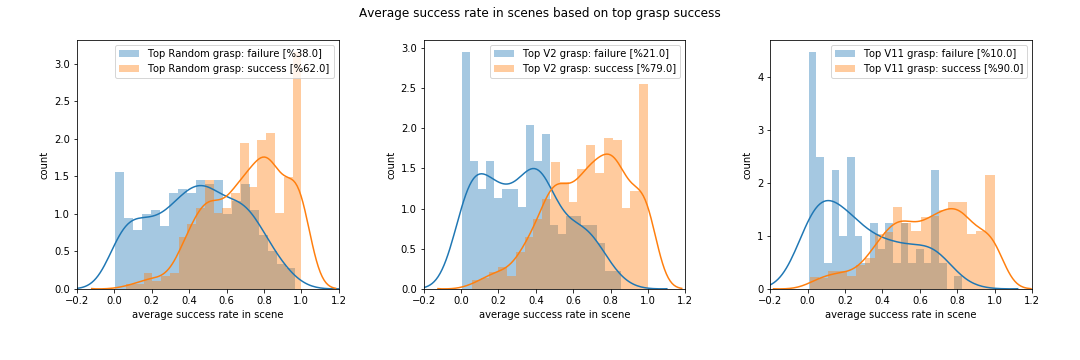
\includegraphics[width=0.8\columnwidth]{images/post-analysis/Average_success_rate_in_scenes_based_on_top_grasp_success.png}
%\caption{Average success rate in scenes vs top grasp success.}
%\label{fig:post7}
%\end{figure}

%\begin{figure}
%\centering
%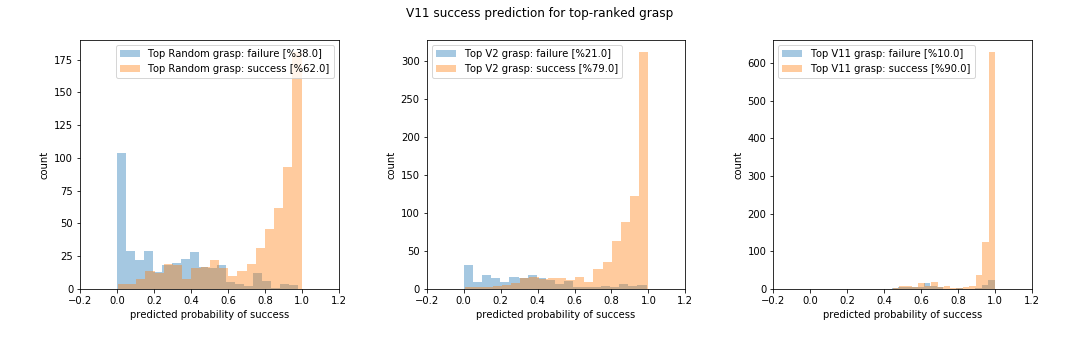
\includegraphics[width=0.8\columnwidth]{images/post-analysis/V11_success_prediction_for_top-ranked_grasp.png}
%\caption{Histogram of success rate of a top-ranked grasp vs its probability of success as estimated by V11.}
%\label{fig:post8}
%\end{figure}

%\begin{figure}
%\centering
%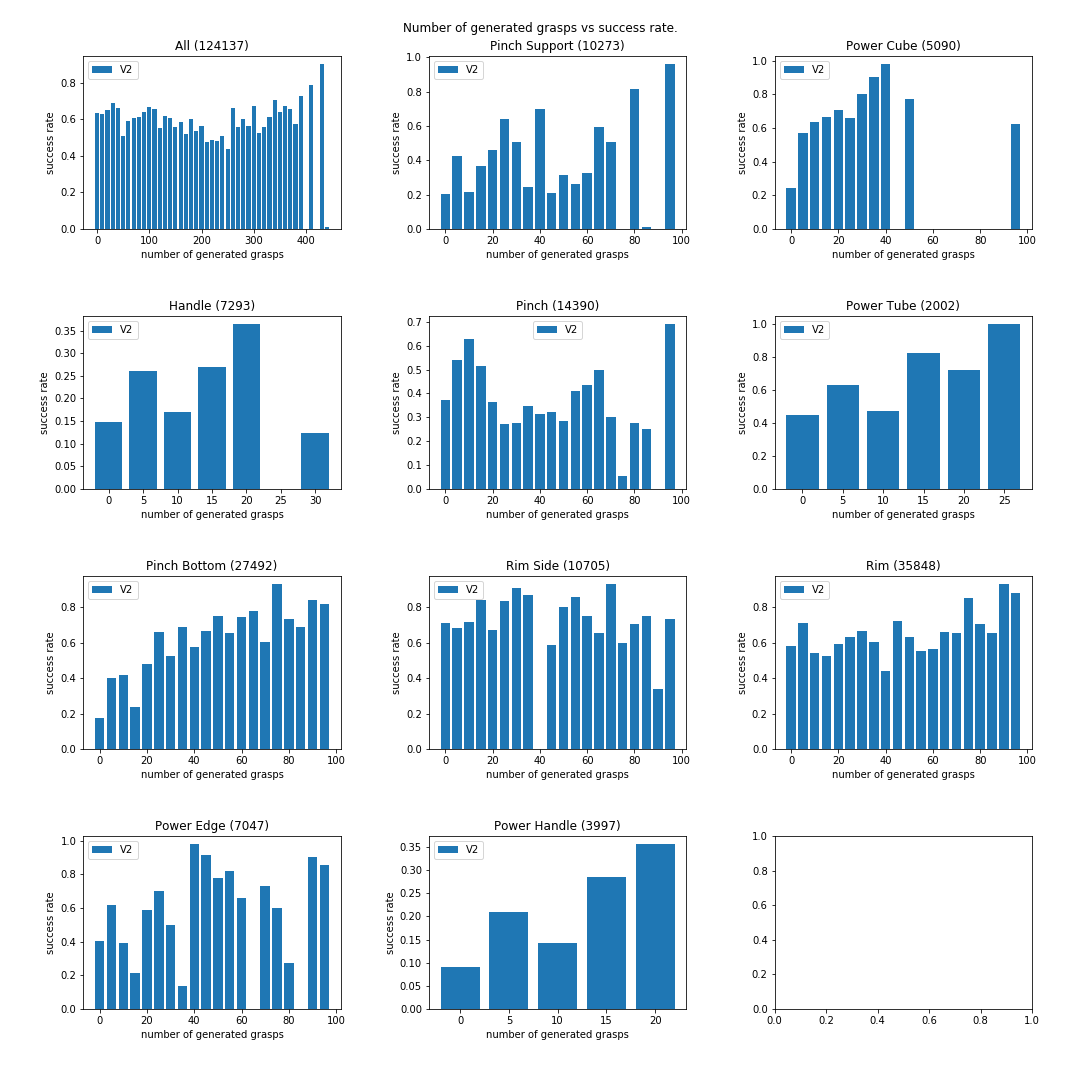
\includegraphics[width=0.8\columnwidth]{images/post-analysis/number_of_generated_grasps_vs_success_rate.png}
%\caption{Correlation of success rate with number of generated grasps per scene per grasp type.}
%\label{fig:post10}
%\end{figure}


%We compared the EM and GM rankings (Figure~\ref{fig:successvsranking}). The x-axis shows the ranking. The y-axis shows the average actual success rate over all scenes (1,241 test, 7,311 training). When ranked by the EM, the grasp success probability falls nearly monotonically, as is desirable. On the other hand, the likelihood-based ranking of GM results in many good grasps being low-ranked. We also wish to know whether the grasps recommended by the EM and the GM have different grasp success rates. The success rates of the top-ranked grasps are 71.59\% (GM) and  84.2\% (EM).

%A pure generative model architecture (GM) and the generative-evaluative architecture (GEA) were evaluated using a paired trials methodology. Each was presented with the same object-pose combinations. Each architecture generated a ranked list of grasps, and the highest ranked grasp was executed. The highest-ranked grasp based on the predicted success probability of the network is performed on each scene. A grasp was deemed successful if, when lifted for five seconds, the object then remained stable in the hand for a further five seconds before being automatically released. The success rate for GM was 57.1\% and for GEA it was 77.6\%. The successes and failures for each method were recorded and are summarised in Table~\ref{tab:robot-results}. A two-tailed McNemar test, for the difference between success rates for paired comparison data, was performed and the difference between the two algorithms has a $p$-value of 0.0442, and so is statistically significant. A selection of grasps where the two methods performed differently are shown in Figure~\ref{fig:successfail}.

% OLD TABLE
%\begin{table}
%\begin{center}
%\caption{Results of the real robot paired comparison trial.}
%\begin{tabular}{|c|c|c|c|}  \hline 
%          &                & \multicolumn{2}{ c |}{ GM} \\ \hline
%          &                & \# succs & \# fails  \\  \hline
 %GEA  & \# succs &  23 &  15  \\
 %         & \# fails    &  5   &   6   \\ \hline
%\end{tabular}
%\end{center}
%\label{tab:robot-results}
%\end{table}

%Training parameters for network. Training of example grasps for learning from demonstration. Creation of real test data set. Paired comparisons methodology with vanilla LFD algorithm (pose + object + camera view).
%
%The actual grasping tests have been performed on the real robot. 

\section{Conclusion} 
\label{sec:conclusion}
This paper has presented the first generative-evaluative architecture for dexterous grasping from a single view in which both the generative and evaluative models are learned. Using this architecture the success rate for the top ranked grasp rises from 69.5\% (for V1) to 90.49\% (for V11) on a simulated test set. It also presented a real robot data set where the top ranked grasp success rate rose from 57.1\% (V1) to 87.8\% (V11).

What are the promising lines of enquiry to further improve dexterous grasping of unfamiliar objects? We see three major issues. First, we have assumed no notion of object completion. Humans succeed in grasping in part because we have strong priors on object shape that help complete the missing information. This would enable the deployment of a generative model that exploits a more complete object shape model \cite{kopicki2015ijrr}. Second, our approach is open-loop during execution. For pinch-grasping, deep nets have been shown to learn useful visual servoing policies \cite{morrison18}. However, significant gains will also come from post-grasp force-control strategies, which are largely absent from the literature on grasp learning.  Third, the architectural scheme presented here is essentially that of an actor-critic architecture. This suggests incremental refinement of both the generative model and the evaluative model, perhaps using techniques from reward based learning. We have already shown elsewhere that the GM may be further improved by training from autonomously generated data \cite{kopicki2019ijrr}. Data intensive generative models also hold promise \cite{veres2017modeling} and it may be possible to seed them by training with example grasps drawn from a data-efficient model such as that presented here.

\section*{Acknowledgements}

The authors gratefully acknowledge funding from the European Commission Funded project, PaCMan FP7-IST-600918.

%\appendix

%\section{Data Efficient Learning of a Generative Grasp Model from Demonstration}

%Describe, in new words, the method from IJRR.
%This section describes the generative model learning. We employ the method of \citet{kopicki2015ijrr}, which learns a generative model of a dexterous grasp from a demonstration (LfD). That paper posed it as the problem of learning a factored probabilistic model. The method is split into a model learning phase, a model transfer phase, and the grasp generation phase. 

\subsection{Model learning}
The model learning is split into three parts: acquiring an {\em object model}; using this object model, with a demonstrated grasp, to build a {\em contact model} for each finger link in contact with the object; and acquiring a {\em hand configuration model} from the demonstrated grasp. After learning the object model can be discarded.

\subsubsection{Object model}
First, a point cloud of the object used for the demonstrated grasp is acquired by a depth camera, from several views. Each point is augmented with the estimated principal curvatures at that point and a surface normal. Thus, the $j^{th}$ point  in the cloud gives rise to a feature $x_j=(p_j, q_j, r_j)$, with the components being its position $p_j \in \mathbb R^3$, orientation $q_j \in SO(3)$ and principal curvatures $r_j=(r_{j,1},r_{j,2}) \in \mathbb R^2$. The orientation $q_j$ is defined by $k_{j,1},k_{j,2}$, which are the directions of the principal curvatures.  For later convenience we use $v=(p,q)$ to denote position and orientation combined. These features $x_j$ allow the object model to be defined as a kernel density estimate of the joint density over $v$ and $r$.
\begin{equation}
\om(v, r) \equiv \pdf^\om(v, r) \simeq \sum_{j=1}^{K_O} w_j \mathcal{K}(v, r|{x_j}, \sigma_{x})
%RD: mu and sigma are not properly defined.
\label{eq:om}
\end{equation}
where $\om$ is short for $\pdf^\om$, bandwidth $\sigma_{x} = (\sigma_{p}, \sigma _{q}, \sigma_{r})$, $K_O$ is the number of features $x_j$ in the object model, all weights are equal $w_j = 1/{K_O}$, and $\mathcal{K}$ is defined as a product:
\begin{equation}\label{eq:kernel_in_se3}
\mathcal{K}(x | \mu, \sigma) = \mathcal{N}_3(p| \mu_p, \sigma_p) \Theta(q| \mu_q, \sigma_q) \mathcal{N}_2(r| \mu_r, \sigma_r)
\end{equation}
where $\mu$ is the kernel mean point, $\sigma$ is the kernel bandwidth, $\mathcal{N}_n$ is an $n$-variate isotropic Gaussian kernel, and ${\Theta}$ corresponds to a pair of antipodal von Mises-Fisher distributions.
\begin{figure*}[t]
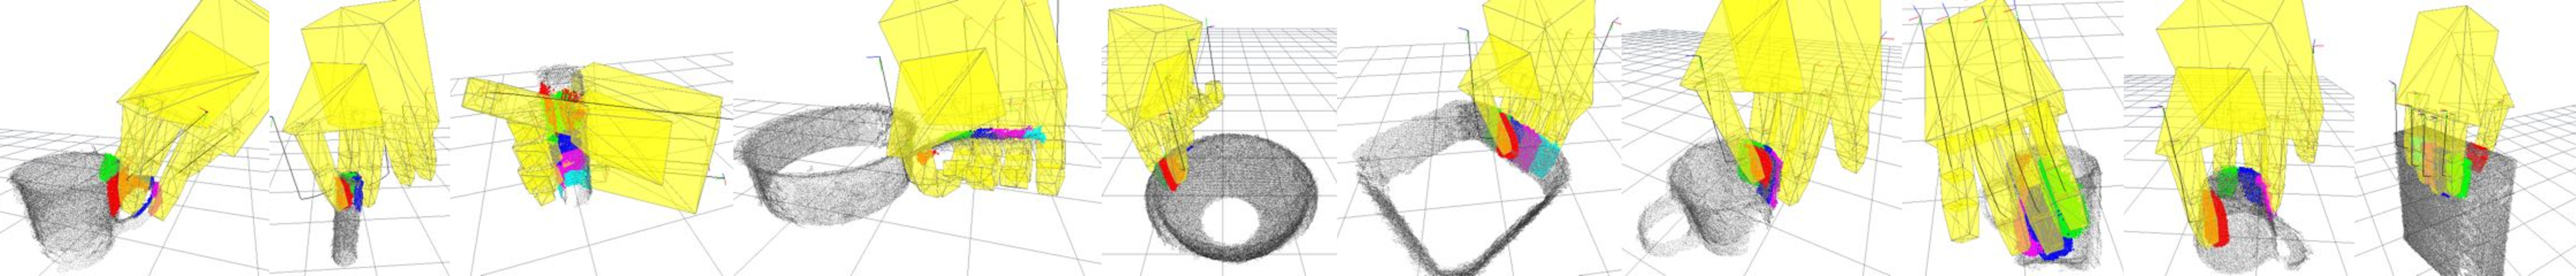
\includegraphics[width=\textwidth]{images/training-examples}
%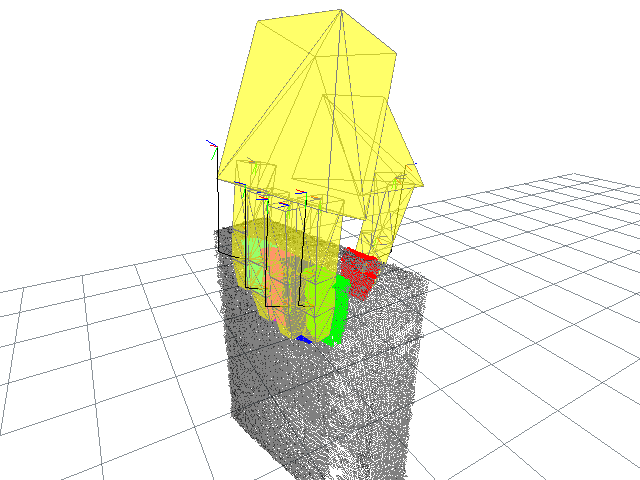
\includegraphics[width=0.1\textwidth]{images/contact-viewall2}
%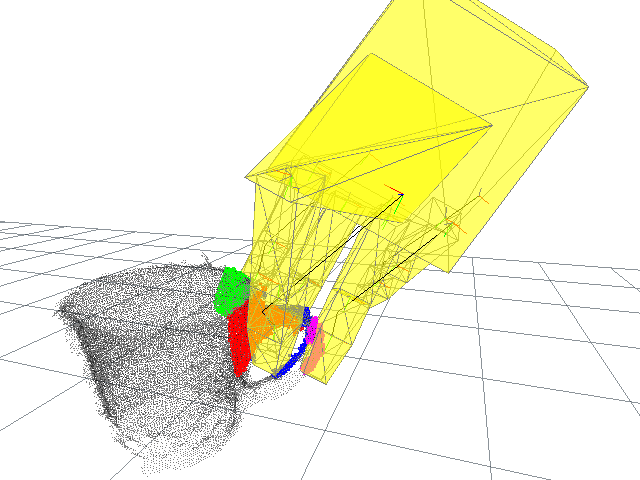
\includegraphics[width=0.1\textwidth]{images/contact-viewall3}
%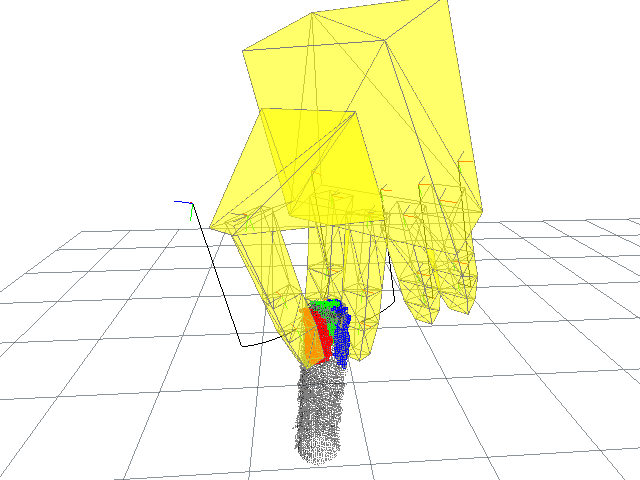
\includegraphics[width=0.1\textwidth]{images/contact-viewall4}
%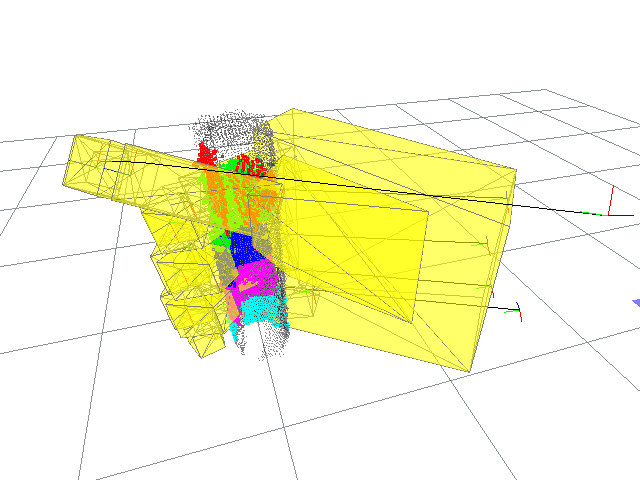
\includegraphics[width=0.1\textwidth]{images/contact-viewall5}
%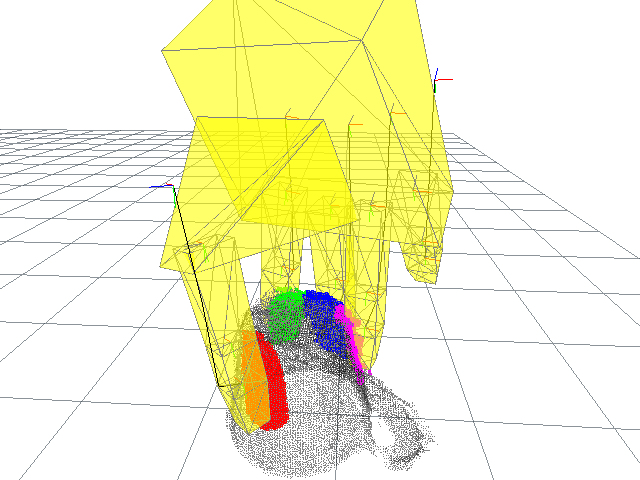
\includegraphics[width=0.1\textwidth]{images/contact-viewall6}
%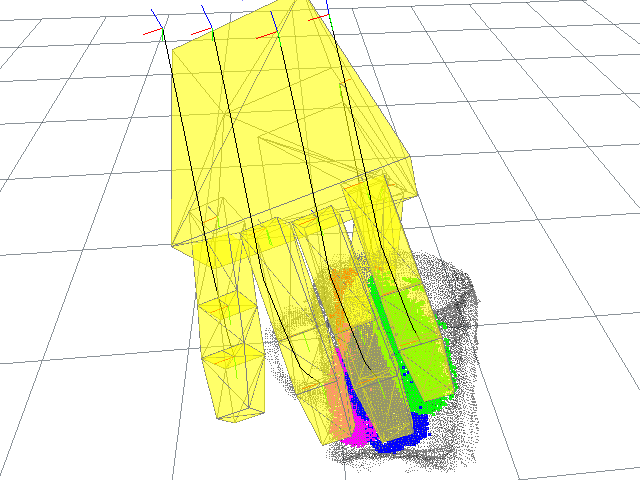
\includegraphics[width=0.1\textwidth]{images/contact-viewall7}
%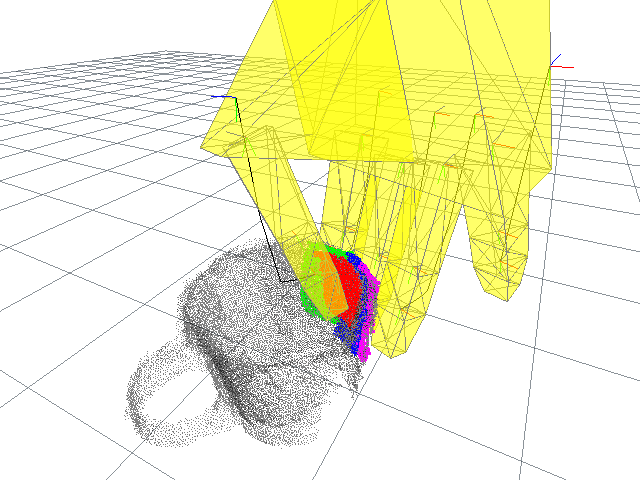
\includegraphics[width=0.1\textwidth]{images/contact-viewall8}
%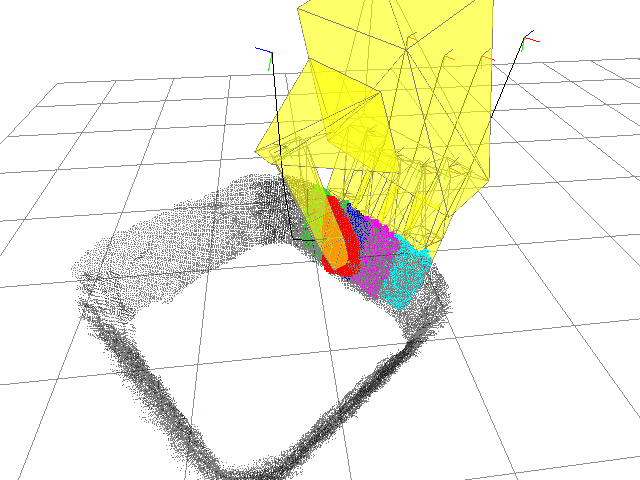
\includegraphics[width=0.1\textwidth]{images/contact-viewall9}
%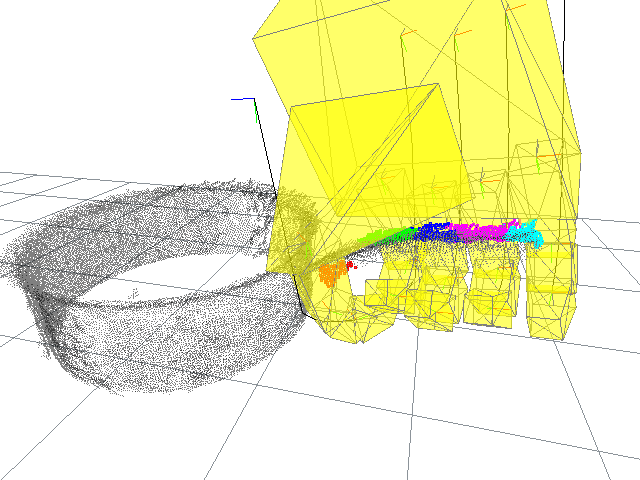
\includegraphics[width=0.1\textwidth]{images/contact-viewall10}
\caption{The ten training grasps for the generative model. The final hand pose is shown in yellow, the sensed point cloud in black, and the parts of the point cloud that contribute to each contact model are coloured by the associated link. \label{fig:generative-training}}
\end{figure*}
\subsubsection{Contact models}
When a grasp is demonstrated the final hand pose is recorded. This is used to find all the finger links $L$ and surface features $x_j$ that are in close proximity. A contact model $M_i$ is built for each finger link $i$. Each feature in the object model that is within some distance $\delta_i$ of finger link $L_i$ contributes to the contact model $\cm_i$ for that link. This contact model is defined for finger link $i$ as follows:
\begin{equation}
\cm_i(u, r) \equiv \pdf^\cm_i(u, r) \simeq \frac{1}{Z} \sum_{j=1}^{K_{M_i}} w_{ij} \mathcal{K}(u, r | {x_j}, \sigma_{x})
%RD: mu and sigma are not properly defined.
\label{eq:cm}
\end{equation}
where $u$ is the pose of $\rl_i$ relative to the pose $v_j$ of the $j^{\mathnormal{th}}$ surface feature, $K_{M_i}$ is the number of surface features in the neighbourhood of link $L_i$, $Z$ is the normalising constant, and $w_{ij}$ is a weight that falls off exponentially as the distance between the feature $x_j$ and the closest point $a_{ij}$ on finger link $L_i$ increases:
\begin{equation}
w_{ij} = \begin{cases}\exp(-\lambda ||p_j-a_{ij}||^2) \quad &\textnormal{ if } ||p_j-a_{ij}|| < \delta_i\\
0 \quad &\textnormal{ otherwise},\end{cases}
\label{eq:learning.modeldist.wgh}
\end{equation}
The key property of a contact model is that it is conditioned on local surface features likely to be found on other objects, so that the grasp can be transferred. We use the principal curvatures $r$, but many local surface descriptors would do. %A contact model can be visualised by marginalising out the dimensions for the rigid body transformation $u$, showing us the distribution over the local curvatures that finger link $L_i$ experienced in the demonstrated grasp. 
%
%\begin{figure*}
%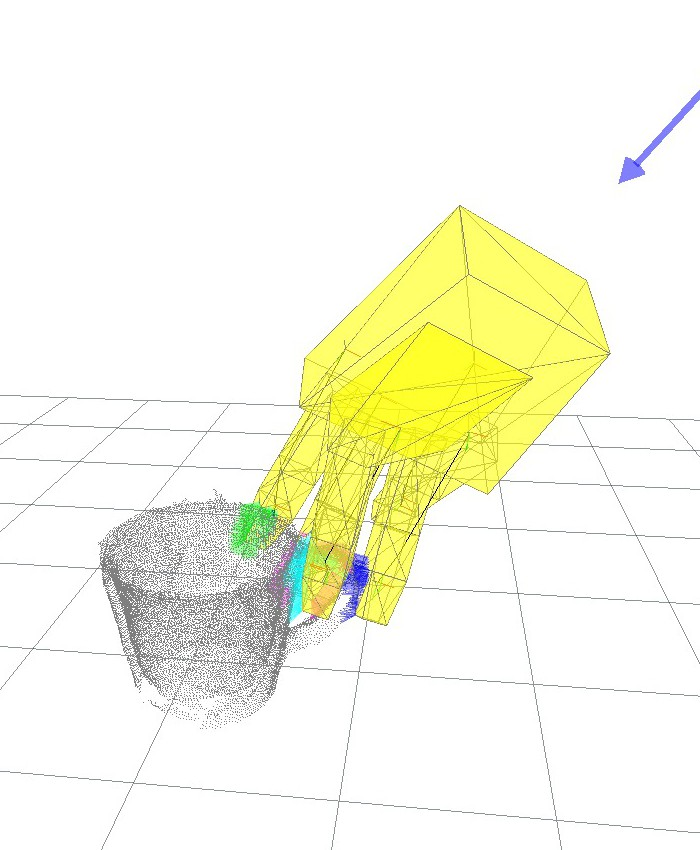
\includegraphics[height=2cm]{images/contact-model-learning/handle-grasp}
%\includegraphics[height=2cm]{images/contact-model-learning/link8}
%\includegraphics[height=2cm]{images/contact-model-learning/handle_model_08_00778r}
%\includegraphics[height=2cm]{images/contact-model-learning/link15}
%\includegraphics[height=2cm]{images/contact-model-learning/handle_model_15_00329r}
%  \caption{A training grasp and some contact models arising from it.}
%  \label{fig:contactModels}
%\end{figure*}

\subsection{Hand configuration model}
In addition to a contact model for each finger-link, a model of the hand configuration $h_c \in \mathbb R^D$ is recorded, where $D$ is the number of DoF in the hand. $h_c$  is recorded for several points on the demonstrated grasp trajectory as the hand closed. The learned model is:
\begin{equation}
\hc(h_c) \equiv \sum_{\gamma \in [-\beta, \beta]} w({h_c(\gamma)}) \mathcal{N}_D(h_c|h_c(\gamma), \sigma_{h_c}) 
\label{eq:hc}
\end{equation}
where $w({h_c(\gamma)}) = \exp(-\alpha \|h_c(\gamma) - h^g_c \|^2)$; $\gamma$ is a parameter that interpolates between the beginning ($h^t_c$) and end ($h^g_c$) points on the trajectory, governed via \eq\ref{eq:learning.configmodel.config} below; and $\beta$ is a parameter that allows extrapolation of the hand configuration.
\begin{equation}
h_c(\gamma) = (1 - \gamma)h^g_c + \gamma h^t_c
\label{eq:learning.configmodel.config}
\end{equation}
\subsection{Grasp Transfer}
When presented with a new object $o_{new}$ the contact models must be transferred to that object. A partial point cloud of $o_{new}$ is acquired (from a single view) and recast as a density, $\om_{new}$, again using \eq \ref{eq:om}. The transfer of each contact model $\cm_i$ is achieved by convolving $\cm_i$ with $\om_{new}$. This convolution is approximated with a Monte-Carlo method, resulting in an kernel density model of the pose $s$ of the finger link $i$ (in workspace coordinates) for the new object. The Monte-Carlo procedure samples poses for link $L_i$ on the new object. The $j^{th}$ sample is $\hat{s}_{ij}=(\hat{p}_{ij},\hat{q}_{ij})$. Each sample $\hat{s}_{ij}$ is weighted $w_{ij}$ by its likelihood. These samples are used to build what we term the query density:
\begin{equation}
\qd_i(s) \simeq \sum^{K_{Q_i}}_{j=1} w_{ij} \mathcal{N}_3(p|{\hat{p}_{ij}}, \sigma_{p}) \Theta(q|{\hat{q}_{ij}}, \sigma_{q})%, \quad i = 1, ..., N_L
\label{eq:qd.approx}
\end{equation}
where all the weights are normalised, $\sum_j w_{ij} = 1$. A query density is constructed for every contact model and the new object. These query densities, together with the hand configuration model, are then used to generate grasps. Query density computation is fast, taking $<0.5$ second per grasp model.
\begin{figure*}[t]
\begin{center}
  \includegraphics[width=0.9\textwidth]{images/networkArchitecture.pdf}
  \end{center}
  \caption{The evaluative network architecture.}
\label{fig:networkArchitecture}
\end{figure*}
\subsection{Grasp generation}
Candidate grasps may be generated as follows. Select a query density $k$ and take a sample  $s_k \sim \qd_{k}$. Then, take a sample $h_c \sim C$ from the hand configuration model. This pair of samples together define, via the hand kinematics, a complete grasp $h=(h_w,h_c)$, where $h_w$ is the pose of the wrist and $h_c$ is the configuration of the hand. The initial grasp is then improved by stochastic hill-climbing on a product of experts:
\begin{equation}
\argmax{(h_w, h_c)} \hc(h_c) \prod_{\qd_i \in \mathcal{Q}} \qd_i\left(k_{i}^{\mathrm{for}}\left(h_w, h_c\right)\right)
\label{eq:grasping.product}
\end{equation}
This generate and improvement process has periodic pruning steps, in which only the higher likelihood grasps are retained. It can be run many times, thus enabling the generation of many candidate grasps. In addition, a separate generative model can be learned for each demonstrated grasp. Thus, when presented with a new object, each grasp model can be used to generate and improve grasps. We generate and optimise 100 grasps per grasp type. Finally, the many candidate grasps generated from each grasp model can be compared and ranked according to their likelihoods. The product of experts formulation, however, only ensures that the generated grasps have high likelihood according to the model. There is no estimate of the probability that the grasp will succeed. This motivates the dual architecture in this paper. We now turn to the learning method we used to re-rank the grasps according to predicted success probability. 

\subsection{Training Grasps for Our Study}

For the purposes of our study, ten example grasps were provided. These are visualised in Figure~\ref{fig:generative-training}. In contrast to \cite{kopicki2015ijrr}, although seven views of each training object were taken, we trained a separate generative model for each view. This led to a total of 70 generative models being learned, one for each grasp-view combination. In addition, we made two innovations to the generative model. In the first, because of the view based training, we filter surface normals on the object model so that for each contact model we only consider points on the object surface with surface normals within +/- 90 degrees of the surface of the finger link. In the second, rather than globally selected the best grasps during optimisation---regardless of the training grasp type, as in the algorithm reported in \cite{kopicki2015ijrr}---we select half globally across all training grasp types, and half we force to be evenly spread across the grasp types. This enables us to keep a broad range of grasp options open to us for evaluation, and thus improves performance.
 \label{section:generative}

%\section{Improved Generative Learning}

%Describe, in new words, the method from IJRR.
%%% This section describes the improved generative method. Only the differences between the original method (given in the previous section) and the new methhod are explained here. 

In this paper we also utilised a more advanced generative model, which we refer to as GM2. This model has four features which are different from the base model GM1. As for GM1 these are not a contribution of this paper and are described fully in \cite{kopicki2019ijrr}. For completeness we briefly describe the three differences between GM2 and GM1. 

\subsection{Object View Model}\label{sec:representations.object}
The first difference is that the learning of grasp models is done per view, rather than per grasp. This means that for a training grasp made on an object viewed from seven viewpoints that there will be seven grasp models learned. This enables grasps to generalise better when the testing object to be grasped is thick and is only seen from a single view. The view based models allow a greater role to be played by the hand shape model and this enables generated grasps to have fingers which `float' behind a back surface that cannot be seen by the robot.

\subsection{Clustering Contact Models}\label{sec:learning.clustering}

The second innovation is the ability to merge grasp models learned from different grasps. Using the memory based scheme of GM1, the number of contact models $N_{\mathcal{M}}$ equals the product of the number of training grasps by the number of views. This has two undesirable properties. First, it means that generation of grasps for test objects rises linearly in the number of training grasps. Second, it limits the generalisation power of the contact models. We can overcome both these problems by clustering the contact models from each training grasp. To do this we need a measure of the similarity between any pair of contact models. Recall that our contact models are probability densities represented as kernel density estimators. Thus, we need a distance metric in the space of probability densities of a given dimension.

One possibility would to employ Jensen-Shannon distance, but this is slow to evaluate. We therefore start by devising a simple asymmetric divergence, which is designed to be quick to compute. We then build on top of it a symmetric distance. Having obtained this distance measure we can employ our clustering method of choice, which in our case was affinity propagation \cite{frey2007clustering}. After clustering, we compute a cluster prototype as described in \cite{kopicki2019}.

\subsection{Improved Grasp Transfer and Inference}
GM2 utilises the same distance measure to transfer grasps when creating the query densities and also to evaluate candidate grasps. This has the effect of making the proposed grasps more conservative and thus closer to the demonstrated grasps in terms of the type of contacts made with the target object.

Having described both generative models we now proceed to describe how we use these to generate a data-set of 2 million simulated dexterous grasps. \label{section:generative_new}

%%PLS. NOTE TEMPLATE HERE SHOWN FOR DIFFERENT STYLES FOR 
%%TEXT IN JOURNALS, BOOKS, REVIEW VOLUME AND PROCS. ETC.
%%AT ACTUAL WORK PLS. TYPE WITHOUT THE \myhead COMMAND. 
%%YOU CAN FOLLOW MY EXAMPLE FOR THE COMMAND OF 
%%\thebibliography AFTER THE \end{document} COMMAND.

\vspace*{-5pt}   %ONLY NECESSARY

\bibliographystyle{IEEEtran}
\bibliography{new_total}%,newbib,main,deepgrasping,references,some_references_by_Chao}
\eject

%%%%%% OUR BACKGROUND

%FIRST AUTHOR
%\vspace*{13pt}
\noindent%
\parbox{5truein}{
\begin{minipage}[b]{1truein}
\centerline{{\psfig{file=images/bio/rusen_bio,width=1in,height=1.25in,clip,keepaspectratio}}}
\end{minipage}
\hfill         %to 2nd column
\begin{minipage}[b]{3.85truein}
{{\bf Umit Rusen Aktas} is a Research Engineer at Blue Prism Ltd. in London. He obtained his PhD in Computer Science from the University of Birmingham in 2018. He received a BSc and MSc in Computer Engineering from METU, Ankara in 2010 and 2013, respectively. He has published two papers at conferences in Computer Vision (ECCV, ICCV). His research interests include machine learning, robot grasping, machine vision and computer graphics.\hfilneg}
\end{minipage}} %close for parbox


%SECOND AUTHOR
\vspace*{13pt}  
\noindent%
\parbox{5truein}{
\begin{minipage}[b]{1truein}
\centerline{{\psfig{file=images/bio/chao_bio,width=1in,height=1.25in,clip,keepaspectratio}}}
\end{minipage}
\hfill %to 2nd column
\begin{minipage}[b]{3.85truein}
{{\bf Chao Zhao} received the B.S. degree from the University of Electronic Science and Technology of China and an MSc in Computer Science from the University of Birmingham, UK, in 2019. He is currently a Research Engineer at the Beijing Research Institute of China Telecom. His research interests include Artificial Intelligence with both probabilistic and deep learning approaches and its application in robotics.\hfilneg}
\end{minipage}} %close for parbox


%THIRD AUTHOR
\vspace*{13pt}  
\noindent%
\parbox{5truein}{
\begin{minipage}[b]{1truein}
\centerline{{\psfig{file=images/bio/marek_bio,width=1in,height=1.25in,clip,keepaspectratio}}}
\end{minipage}
\hfill %to 2nd column
\begin{minipage}[b]{3.85truein}
{{\bf Marek Kopicki} is a senior research engineer at Dyson. He has a MSc in physics from Adam Mickiewicz University (Poznan), a MSc in Advance Computer Science and Ph.D. in robotics at University of Birmingham in 2010. He has more than twelve years’ experience of developing algorithms and software for robot control and vision. These were used in  FP7 projects CogX, GeRT and PaCMan. He invented an adaptive grasping algorithm, for which he holds an international patent. He has published more than twenty-five refereed papers.\hfilneg}
\end{minipage}} %close for parbox


%FOURTH AUTHOR
\vspace*{13pt}  
\noindent%
\parbox{5truein}{
\begin{minipage}[b]{1truein}
\centerline{{\psfig{file=images/bio/ales_bio,width=1in,height=1.25in,clip,keepaspectratio}}}
\end{minipage}
\hfill %to 2nd column
\begin{minipage}[b]{3.85truein}
{{\bf Ales Leonardis} is a Professor of Robotics at University of Birmingham. He is also an adjunct professor at the Faculty of Computer Science, Graz University of Technology. His research interests include robust and adaptive methods for computer vision, object and scene recognition and categorization, statistical visual learning, 3D object modeling, and biologically motivated vision. He is a fellow of the IAPR and a member of the IEEE and the IEEE Computer Society. \hfilneg}
\end{minipage}} %close for parbox


%FIFTH AUTHOR
\vspace*{13pt}  
\noindent%
\parbox{5truein}{
\begin{minipage}[b]{1truein}
\centerline{{\psfig{file=images/bio/jeremy,width=1in,height=1.25in,clip,keepaspectratio}}}
\end{minipage}
\hfill %to 2nd column
\begin{minipage}[b]{3.85truein}
{{\bf Jeremy L. Wyatt}
received a B.A. in Theology from University of Bristol, an M.Sc. in Artificial Intelligence from University of Sussex, and his Ph.D. in Machine Learning from the University of Edinburgh in 1997. He is Honorary Professor of Robotics and Artificial Intelligence at the University of Birmingham, Birmingham. He has published more than 100 papers, edited three books, received two best paper awards, supervised a BCS distinguished doctoral dissertation, and led a variety of research projects. His research interests include robot task planning, statistical machine learning, and robot manipulation. \hfilneg}
\end{minipage}} %close for parbox


\vfill\eject

\end{document}

